\documentclass[twoside]{book}

% Packages required by doxygen
\usepackage{fixltx2e}
\usepackage{calc}
\usepackage{doxygen}
\usepackage[export]{adjustbox} % also loads graphicx
\usepackage{graphicx}
\usepackage[utf8]{inputenc}
\usepackage{makeidx}
\usepackage{multicol}
\usepackage{multirow}
\PassOptionsToPackage{warn}{textcomp}
\usepackage{textcomp}
\usepackage[nointegrals]{wasysym}
\usepackage[table]{xcolor}

% NLS support packages
\usepackage[T2A]{fontenc}
\usepackage[russian]{babel}

% Font selection
\usepackage[T1]{fontenc}
\usepackage[scaled=.90]{helvet}
\usepackage{courier}
\usepackage{amssymb}
\usepackage{sectsty}
\renewcommand{\familydefault}{\sfdefault}
\allsectionsfont{%
  \fontseries{bc}\selectfont%
  \color{darkgray}%
}
\renewcommand{\DoxyLabelFont}{%
  \fontseries{bc}\selectfont%
  \color{darkgray}%
}
\newcommand{\+}{\discretionary{\mbox{\scriptsize$\hookleftarrow$}}{}{}}

% Page & text layout
\usepackage{geometry}
\geometry{%
  a4paper,%
  top=2.5cm,%
  bottom=2.5cm,%
  left=2.5cm,%
  right=2.5cm%
}
\tolerance=750
\hfuzz=15pt
\hbadness=750
\setlength{\emergencystretch}{15pt}
\setlength{\parindent}{0cm}
\setlength{\parskip}{3ex plus 2ex minus 2ex}
\makeatletter
\renewcommand{\paragraph}{%
  \@startsection{paragraph}{4}{0ex}{-1.0ex}{1.0ex}{%
    \normalfont\normalsize\bfseries\SS@parafont%
  }%
}
\renewcommand{\subparagraph}{%
  \@startsection{subparagraph}{5}{0ex}{-1.0ex}{1.0ex}{%
    \normalfont\normalsize\bfseries\SS@subparafont%
  }%
}
\makeatother

% Headers & footers
\usepackage{fancyhdr}
\pagestyle{fancyplain}
\fancyhead[LE]{\fancyplain{}{\bfseries\thepage}}
\fancyhead[CE]{\fancyplain{}{}}
\fancyhead[RE]{\fancyplain{}{\bfseries\leftmark}}
\fancyhead[LO]{\fancyplain{}{\bfseries\rightmark}}
\fancyhead[CO]{\fancyplain{}{}}
\fancyhead[RO]{\fancyplain{}{\bfseries\thepage}}
\fancyfoot[LE]{\fancyplain{}{}}
\fancyfoot[CE]{\fancyplain{}{}}
\fancyfoot[RE]{\fancyplain{}{\bfseries\scriptsize Создано системой Doxygen }}
\fancyfoot[LO]{\fancyplain{}{\bfseries\scriptsize Создано системой Doxygen }}
\fancyfoot[CO]{\fancyplain{}{}}
\fancyfoot[RO]{\fancyplain{}{}}
\renewcommand{\footrulewidth}{0.4pt}
\renewcommand{\chaptermark}[1]{%
  \markboth{#1}{}%
}
\renewcommand{\sectionmark}[1]{%
  \markright{\thesection\ #1}%
}

% Indices & bibliography
\usepackage{natbib}
\usepackage[titles]{tocloft}
\setcounter{tocdepth}{3}
\setcounter{secnumdepth}{5}
\makeindex

% Hyperlinks (required, but should be loaded last)
\usepackage{ifpdf}
\ifpdf
  \usepackage[pdftex,pagebackref=true]{hyperref}
\else
  \usepackage[ps2pdf,pagebackref=true]{hyperref}
\fi
\hypersetup{%
  colorlinks=true,%
  linkcolor=blue,%
  citecolor=blue,%
  unicode%
}

% Custom commands
\newcommand{\clearemptydoublepage}{%
  \newpage{\pagestyle{empty}\cleardoublepage}%
}

\usepackage{caption}
\captionsetup{labelsep=space,justification=centering,font={bf},singlelinecheck=off,skip=4pt,position=top}

%===== C O N T E N T S =====

\begin{document}

% Titlepage & ToC
\hypersetup{pageanchor=false,
             bookmarksnumbered=true,
             pdfencoding=unicode
            }
\pagenumbering{alph}
\begin{titlepage}
\vspace*{7cm}
\begin{center}%
{\Large СКОП 2.01 \\[1ex]\large A21.\+07 -\/ 31.\+07.\+2021 }\\
\vspace*{1cm}
{\large Создано системой Doxygen 1.8.13}\\
\end{center}
\end{titlepage}
\clearemptydoublepage
\pagenumbering{roman}
\tableofcontents
\clearemptydoublepage
\pagenumbering{arabic}
\hypersetup{pageanchor=true}

%--- Begin generated contents ---
\chapter{Список задач}
\label{todo}
\Hypertarget{todo}

\begin{DoxyRefList}
\item[\label{todo__todo000003}%
\Hypertarget{todo__todo000003}%
Член \hyperlink{group___xD0_x9F_xD0_xB5_xD1_x80_xD0_xB5_xD1_x87_xD0_xB8_xD1_x81_xD0_xBB_xD0_xB5_xD0_xBD_xD0_xB8_xD1_x8F_ga290e8080c661e52c2f685fd4af148acf}{app\+:\+:app\+State} ]Найти оптимальный размер диска для работы с SD карточкой и разобраться с работой S\+D\+IO по D\+MA 

Убрать Fat\+FS и сделать свою работу с карточкой  
\item[\label{todo__todo000002}%
\Hypertarget{todo__todo000002}%
Член \hyperlink{classapp_1_1_t_application_a0c44fe0e56bc2d85720155880c9b54a6}{app\+:\+:T\+Application\+:\+:debug\+Mesage} (const uint8\+\_\+t $\ast$, const std\+::size\+\_\+t)]Переделать на хрен на потоковый вывод  
\item[\label{todo__todo000001}%
\Hypertarget{todo__todo000001}%
Член \hyperlink{classapp_1_1_t_application_a2ac87a63360e7974afe2249f7b7e54cd}{app\+:\+:T\+Application\+:\+:debug\+Mesage} (const std\+::string \&)]Переделать на хрен на потоковый вывод  
\item[\label{todo__todo000004}%
\Hypertarget{todo__todo000004}%
Член \hyperlink{classunit_1_1_t_file_system_a0737b50d219570ae2e11ea17a32cc85c}{unit\+:\+:T\+File\+System\+:\+:check} ()]Приделать проверку записи и чтения тестового файла  
\item[\label{todo__todo000005}%
\Hypertarget{todo__todo000005}%
Класс \hyperlink{classunit_1_1_t_photo}{unit\+:\+:T\+Photo} ]Убрать ov2640.\+c и передалать на плюсы (Хотя не очень понятно зачем???) 

Убрать все Warning в ov2640.\+c 
\end{DoxyRefList}
\chapter{Алфавитный указатель групп}
\section{Группы}
Полный список групп.\begin{DoxyCompactList}
\item \contentsline{section}{Обработчики прерываний}{\pageref{group___callback}}{}
\item \contentsline{section}{Перечисления}{\pageref{group___xD0_x9F_xD0_xB5_xD1_x80_xD0_xB5_xD1_x87_xD0_xB8_xD1_x81_xD0_xBB_xD0_xB5_xD0_xBD_xD0_xB8_xD1_x8F}}{}
\end{DoxyCompactList}

\chapter{Алфавитный указатель пространств имен}
\section{Пространства имен}
Полный список документированных пространств имен.\begin{DoxyCompactList}
\item\contentsline{section}{\hyperlink{namespaceapp}{app} \\*Всё, что касается управления приложением }{\pageref{namespaceapp}}{}
\item\contentsline{section}{\hyperlink{namespacecommon}{common} \\*Различные общие для всего приложения определения }{\pageref{namespacecommon}}{}
\item\contentsline{section}{\hyperlink{namespaceunit}{unit} \\*Всё, что касается работы управления внешними чипами }{\pageref{namespaceunit}}{}
\end{DoxyCompactList}

\chapter{Иерархический список классов}
\section{Иерархия классов}
Иерархия классов.\begin{DoxyCompactList}
\item \contentsline{section}{app\+:\+:T\+Application}{\pageref{classapp_1_1_t_application}}{}
\item \contentsline{section}{app\+:\+:T\+Button}{\pageref{classapp_1_1_t_button}}{}
\item \contentsline{section}{unit\+:\+:T\+Unit}{\pageref{classunit_1_1_t_unit}}{}
\begin{DoxyCompactList}
\item \contentsline{section}{unit\+:\+:T\+Audio}{\pageref{classunit_1_1_t_audio}}{}
\item \contentsline{section}{unit\+:\+:T\+Bq25121}{\pageref{classunit_1_1_t_bq25121}}{}
\item \contentsline{section}{unit\+:\+:T\+File\+System}{\pageref{classunit_1_1_t_file_system}}{}
\item \contentsline{section}{unit\+:\+:T\+I2C}{\pageref{classunit_1_1_t_i2_c}}{}
\item \contentsline{section}{unit\+:\+:T\+Photo}{\pageref{classunit_1_1_t_photo}}{}
\item \contentsline{section}{unit\+:\+:T\+Sdio}{\pageref{classunit_1_1_t_sdio}}{}
\item \contentsline{section}{unit\+:\+:T\+Tag}{\pageref{classunit_1_1_t_tag}}{}
\end{DoxyCompactList}
\end{DoxyCompactList}

\chapter{Алфавитный указатель классов}
\section{Классы}
Классы с их кратким описанием.\begin{DoxyCompactList}
\item\contentsline{section}{\hyperlink{structunit_1_1_audio___buffer_type_def}{unit\+::\+Audio\+\_\+\+Buffer\+Type\+Def} \\*\begin{quote}
Задержка начала записи для устранения посторонних звуков \end{quote}
}{\pageref{structunit_1_1_audio___buffer_type_def}}{}
\item\contentsline{section}{\hyperlink{classapp_1_1_t_application}{app\+::\+T\+Application} \\*Класс содержащий данные для обеспечения работы приложения }{\pageref{classapp_1_1_t_application}}{}
\item\contentsline{section}{\hyperlink{classunit_1_1_t_audio}{unit\+::\+T\+Audio} }{\pageref{classunit_1_1_t_audio}}{}
\item\contentsline{section}{\hyperlink{classunit_1_1_t_bq25121}{unit\+::\+T\+Bq25121} }{\pageref{classunit_1_1_t_bq25121}}{}
\item\contentsline{section}{\hyperlink{classapp_1_1_t_button}{app\+::\+T\+Button} \\*Класс для работы с кнопками }{\pageref{classapp_1_1_t_button}}{}
\item\contentsline{section}{\hyperlink{structapp_1_1td_log_item}{app\+::td\+Log\+Item} \\*Описание структуры для хранения одной записи лога }{\pageref{structapp_1_1td_log_item}}{}
\item\contentsline{section}{\hyperlink{classunit_1_1_t_file_system}{unit\+::\+T\+File\+System} \\*Класс для работы с файловой системой }{\pageref{classunit_1_1_t_file_system}}{}
\item\contentsline{section}{\hyperlink{classunit_1_1_t_i2_c}{unit\+::\+T\+I2C} }{\pageref{classunit_1_1_t_i2_c}}{}
\item\contentsline{section}{\hyperlink{classapp_1_1_t_log}{app\+::\+T\+Log} \\*Класс ведения лога работы }{\pageref{classapp_1_1_t_log}}{}
\item\contentsline{section}{\hyperlink{classunit_1_1_t_photo}{unit\+::\+T\+Photo} }{\pageref{classunit_1_1_t_photo}}{}
\item\contentsline{section}{\hyperlink{classunit_1_1_t_sdio}{unit\+::\+T\+Sdio} }{\pageref{classunit_1_1_t_sdio}}{}
\item\contentsline{section}{\hyperlink{classunit_1_1_t_tag}{unit\+::\+T\+Tag} }{\pageref{classunit_1_1_t_tag}}{}
\item\contentsline{section}{\hyperlink{classunit_1_1_t_unit}{unit\+::\+T\+Unit} }{\pageref{classunit_1_1_t_unit}}{}
\item\contentsline{section}{\hyperlink{struct_w_a_v_e___format_type_def}{W\+A\+V\+E\+\_\+\+Format\+Type\+Def} }{\pageref{struct_w_a_v_e___format_type_def}}{}
\end{DoxyCompactList}

\chapter{Группы}
\hypertarget{group___callback}{}\section{Обработчики прерываний}
\label{group___callback}\index{Обработчики прерываний@{Обработчики прерываний}}
\subsection*{Функции}
\begin{DoxyCompactItemize}
\item 
void \hyperlink{group___callback_ga8a3b0ad512a6e6c6157440b68d395eac}{H\+A\+L\+\_\+\+T\+I\+M\+\_\+\+Period\+Elapsed\+Callback} (T\+I\+M\+\_\+\+Handle\+Type\+Def $\ast$htim)
\begin{DoxyCompactList}\small\item\em Обработчик прерываний от таймера \end{DoxyCompactList}\item 
void \hyperlink{group___callback_gabcdf9b59049eccbc87d54042f9235b1a}{H\+A\+L\+\_\+\+U\+A\+R\+T\+\_\+\+Tx\+Cplt\+Callback} (U\+A\+R\+T\+\_\+\+Handle\+Type\+Def $\ast$huart)
\begin{DoxyCompactList}\small\item\em Обработчик прерываний U\+A\+RT. \end{DoxyCompactList}\end{DoxyCompactItemize}


\subsection{Подробное описание}


\subsection{Функции}
\mbox{\Hypertarget{group___callback_ga8a3b0ad512a6e6c6157440b68d395eac}\label{group___callback_ga8a3b0ad512a6e6c6157440b68d395eac}} 
\index{Обработчики прерываний@{Обработчики прерываний}!H\+A\+L\+\_\+\+T\+I\+M\+\_\+\+Period\+Elapsed\+Callback@{H\+A\+L\+\_\+\+T\+I\+M\+\_\+\+Period\+Elapsed\+Callback}}
\index{H\+A\+L\+\_\+\+T\+I\+M\+\_\+\+Period\+Elapsed\+Callback@{H\+A\+L\+\_\+\+T\+I\+M\+\_\+\+Period\+Elapsed\+Callback}!Обработчики прерываний@{Обработчики прерываний}}
\subsubsection{\texorpdfstring{H\+A\+L\+\_\+\+T\+I\+M\+\_\+\+Period\+Elapsed\+Callback()}{HAL\_TIM\_PeriodElapsedCallback()}}
{\footnotesize\ttfamily void H\+A\+L\+\_\+\+T\+I\+M\+\_\+\+Period\+Elapsed\+Callback (\begin{DoxyParamCaption}\item[{T\+I\+M\+\_\+\+Handle\+Type\+Def $\ast$}]{htim }\end{DoxyParamCaption})}



Обработчик прерываний от таймера 


\begin{DoxyParams}{Аргументы}
{\em htim} & Сработавший таймер\\
\hline
\end{DoxyParams}
T\+I\+M7 -\/ базовый таймер на 1 мСек. \mbox{\Hypertarget{group___callback_gabcdf9b59049eccbc87d54042f9235b1a}\label{group___callback_gabcdf9b59049eccbc87d54042f9235b1a}} 
\index{Обработчики прерываний@{Обработчики прерываний}!H\+A\+L\+\_\+\+U\+A\+R\+T\+\_\+\+Tx\+Cplt\+Callback@{H\+A\+L\+\_\+\+U\+A\+R\+T\+\_\+\+Tx\+Cplt\+Callback}}
\index{H\+A\+L\+\_\+\+U\+A\+R\+T\+\_\+\+Tx\+Cplt\+Callback@{H\+A\+L\+\_\+\+U\+A\+R\+T\+\_\+\+Tx\+Cplt\+Callback}!Обработчики прерываний@{Обработчики прерываний}}
\subsubsection{\texorpdfstring{H\+A\+L\+\_\+\+U\+A\+R\+T\+\_\+\+Tx\+Cplt\+Callback()}{HAL\_UART\_TxCpltCallback()}}
{\footnotesize\ttfamily void H\+A\+L\+\_\+\+U\+A\+R\+T\+\_\+\+Tx\+Cplt\+Callback (\begin{DoxyParamCaption}\item[{U\+A\+R\+T\+\_\+\+Handle\+Type\+Def $\ast$}]{huart }\end{DoxyParamCaption})}



Обработчик прерываний U\+A\+RT. 


\begin{DoxyParams}{Аргументы}
{\em huart} & Хэнвд сработавшего порта \\
\hline
\end{DoxyParams}
\begin{DoxyAttention}{Внимание}
И на хрена он нужен??? 
\end{DoxyAttention}

\hypertarget{group___xD0_x9F_xD0_xB5_xD1_x80_xD0_xB5_xD1_x87_xD0_xB8_xD1_x81_xD0_xBB_xD0_xB5_xD0_xBD_xD0_xB8_xD1_x8F}{}\section{Перечисления}
\label{group___xD0_x9F_xD0_xB5_xD1_x80_xD0_xB5_xD1_x87_xD0_xB8_xD1_x81_xD0_xBB_xD0_xB5_xD0_xBD_xD0_xB8_xD1_x8F}\index{Перечисления@{Перечисления}}
\subsection*{Перечисления}
\begin{DoxyCompactItemize}
\item 
enum \hyperlink{group___xD0_x9F_xD0_xB5_xD1_x80_xD0_xB5_xD1_x87_xD0_xB8_xD1_x81_xD0_xBB_xD0_xB5_xD0_xBD_xD0_xB8_xD1_x8F_ga290e8080c661e52c2f685fd4af148acf}{app\+::app\+State} \{ \newline
\hyperlink{group___xD0_x9F_xD0_xB5_xD1_x80_xD0_xB5_xD1_x87_xD0_xB8_xD1_x81_xD0_xBB_xD0_xB5_xD0_xBD_xD0_xB8_xD1_x8F_gga290e8080c661e52c2f685fd4af148acfafba3da9bcc34395d19f8704220660bf7}{app\+::app\+Unknown} = 0, 
\hyperlink{group___xD0_x9F_xD0_xB5_xD1_x80_xD0_xB5_xD1_x87_xD0_xB8_xD1_x81_xD0_xBB_xD0_xB5_xD0_xBD_xD0_xB8_xD1_x8F_gga290e8080c661e52c2f685fd4af148acfa06429e3f15123c01cc678c167cc05b8b}{app\+::app\+Started}, 
\hyperlink{group___xD0_x9F_xD0_xB5_xD1_x80_xD0_xB5_xD1_x87_xD0_xB8_xD1_x81_xD0_xBB_xD0_xB5_xD0_xBD_xD0_xB8_xD1_x8F_gga290e8080c661e52c2f685fd4af148acfa4cf039e664fb2026ab3fd90d0a51050b}{app\+::app\+Stand\+By}, 
\hyperlink{group___xD0_x9F_xD0_xB5_xD1_x80_xD0_xB5_xD1_x87_xD0_xB8_xD1_x81_xD0_xBB_xD0_xB5_xD0_xBD_xD0_xB8_xD1_x8F_gga290e8080c661e52c2f685fd4af148acfa7703d6d19f36dc6ada3ce7b8e3be5a23}{app\+::app\+Ready}, 
\newline
\hyperlink{group___xD0_x9F_xD0_xB5_xD1_x80_xD0_xB5_xD1_x87_xD0_xB8_xD1_x81_xD0_xBB_xD0_xB5_xD0_xBD_xD0_xB8_xD1_x8F_gga290e8080c661e52c2f685fd4af148acfae13f6f6403aa802b7802fb9d6defd008}{app\+::app\+Audio}, 
\hyperlink{group___xD0_x9F_xD0_xB5_xD1_x80_xD0_xB5_xD1_x87_xD0_xB8_xD1_x81_xD0_xBB_xD0_xB5_xD0_xBD_xD0_xB8_xD1_x8F_gga290e8080c661e52c2f685fd4af148acfac9780bfeff75ce5754c1557da55fb8b0}{app\+::app\+Audio\+Wait\+Stop}, 
\hyperlink{group___xD0_x9F_xD0_xB5_xD1_x80_xD0_xB5_xD1_x87_xD0_xB8_xD1_x81_xD0_xBB_xD0_xB5_xD0_xBD_xD0_xB8_xD1_x8F_gga290e8080c661e52c2f685fd4af148acfa6c6a194d643920afd30bf8f10e6658db}{app\+::app\+Audio\+Stop}, 
\hyperlink{group___xD0_x9F_xD0_xB5_xD1_x80_xD0_xB5_xD1_x87_xD0_xB8_xD1_x81_xD0_xBB_xD0_xB5_xD0_xBD_xD0_xB8_xD1_x8F_gga290e8080c661e52c2f685fd4af148acfa9ef71d54d0a6d2e454e96e97c047bcc6}{app\+::app\+Photo}, 
\newline
\hyperlink{group___xD0_x9F_xD0_xB5_xD1_x80_xD0_xB5_xD1_x87_xD0_xB8_xD1_x81_xD0_xBB_xD0_xB5_xD0_xBD_xD0_xB8_xD1_x8F_gga290e8080c661e52c2f685fd4af148acfa6ece4969fa6384847ee632f9fd55e124}{app\+::app\+Photo\+Button\+Press}, 
\hyperlink{group___xD0_x9F_xD0_xB5_xD1_x80_xD0_xB5_xD1_x87_xD0_xB8_xD1_x81_xD0_xBB_xD0_xB5_xD0_xBD_xD0_xB8_xD1_x8F_gga290e8080c661e52c2f685fd4af148acfae597d89c5bbd7f9873f7fa369ef24df6}{app\+::app\+Photo\+I2\+C\+Err}, 
\hyperlink{group___xD0_x9F_xD0_xB5_xD1_x80_xD0_xB5_xD1_x87_xD0_xB8_xD1_x81_xD0_xBB_xD0_xB5_xD0_xBD_xD0_xB8_xD1_x8F_gga290e8080c661e52c2f685fd4af148acfacaecf479ee7651cb23d3ecfca43f3ddd}{app\+::app\+Photo\+Timeout}, 
\hyperlink{group___xD0_x9F_xD0_xB5_xD1_x80_xD0_xB5_xD1_x87_xD0_xB8_xD1_x81_xD0_xBB_xD0_xB5_xD0_xBD_xD0_xB8_xD1_x8F_gga290e8080c661e52c2f685fd4af148acfa3c31d143e9bc2e3d48ba23ae8bfe01d5}{app\+::app\+Tag}, 
\newline
\hyperlink{group___xD0_x9F_xD0_xB5_xD1_x80_xD0_xB5_xD1_x87_xD0_xB8_xD1_x81_xD0_xBB_xD0_xB5_xD0_xBD_xD0_xB8_xD1_x8F_gga290e8080c661e52c2f685fd4af148acfa25d59b57a27a13e034cab5faf26fd4e0}{app\+::app\+Tag\+Err}, 
\hyperlink{group___xD0_x9F_xD0_xB5_xD1_x80_xD0_xB5_xD1_x87_xD0_xB8_xD1_x81_xD0_xBB_xD0_xB5_xD0_xBD_xD0_xB8_xD1_x8F_gga290e8080c661e52c2f685fd4af148acfaccc67d66e13249dc4fa22d624ce013d4}{app\+::app\+Doc}, 
\hyperlink{group___xD0_x9F_xD0_xB5_xD1_x80_xD0_xB5_xD1_x87_xD0_xB8_xD1_x81_xD0_xBB_xD0_xB5_xD0_xBD_xD0_xB8_xD1_x8F_gga290e8080c661e52c2f685fd4af148acfa50b594306c1d7a073119a0a7bb94a56b}{app\+::app\+Doc\+Wait\+Stop}, 
\hyperlink{group___xD0_x9F_xD0_xB5_xD1_x80_xD0_xB5_xD1_x87_xD0_xB8_xD1_x81_xD0_xBB_xD0_xB5_xD0_xBD_xD0_xB8_xD1_x8F_gga290e8080c661e52c2f685fd4af148acfae29d9127eb593964667686b495588ecf}{app\+::app\+Check\+Bounce}, 
\newline
\hyperlink{group___xD0_x9F_xD0_xB5_xD1_x80_xD0_xB5_xD1_x87_xD0_xB8_xD1_x81_xD0_xBB_xD0_xB5_xD0_xBD_xD0_xB8_xD1_x8F_gga290e8080c661e52c2f685fd4af148acfa336edab4342b86e8be3ec106f44c65ae}{app\+::app\+Check\+Button}, 
\hyperlink{group___xD0_x9F_xD0_xB5_xD1_x80_xD0_xB5_xD1_x87_xD0_xB8_xD1_x81_xD0_xBB_xD0_xB5_xD0_xBD_xD0_xB8_xD1_x8F_gga290e8080c661e52c2f685fd4af148acfadbe7c90fff8efa5ca2cc07d3f442a855}{app\+::app\+Bounce\+Timeout}, 
\hyperlink{group___xD0_x9F_xD0_xB5_xD1_x80_xD0_xB5_xD1_x87_xD0_xB8_xD1_x81_xD0_xBB_xD0_xB5_xD0_xBD_xD0_xB8_xD1_x8F_gga290e8080c661e52c2f685fd4af148acfa89156a1ccc6c5519c84c8f043e8bdc23}{app\+::app\+Start\+Bounce}, 
\hyperlink{group___xD0_x9F_xD0_xB5_xD1_x80_xD0_xB5_xD1_x87_xD0_xB8_xD1_x81_xD0_xBB_xD0_xB5_xD0_xBD_xD0_xB8_xD1_x8F_gga290e8080c661e52c2f685fd4af148acfaaa919407add286f45f3d2f1efec97654}{app\+::app\+Err\+Button}, 
\newline
\hyperlink{group___xD0_x9F_xD0_xB5_xD1_x80_xD0_xB5_xD1_x87_xD0_xB8_xD1_x81_xD0_xBB_xD0_xB5_xD0_xBD_xD0_xB8_xD1_x8F_gga290e8080c661e52c2f685fd4af148acfa14b4efaea15974df40b9d19ecb746d99}{app\+::app\+Err\+I2C}, 
\hyperlink{group___xD0_x9F_xD0_xB5_xD1_x80_xD0_xB5_xD1_x87_xD0_xB8_xD1_x81_xD0_xBB_xD0_xB5_xD0_xBD_xD0_xB8_xD1_x8F_gga290e8080c661e52c2f685fd4af148acfac320769ad532ac30ed4846a8503f4e2f}{app\+::app\+Err\+Bq25121}, 
\hyperlink{group___xD0_x9F_xD0_xB5_xD1_x80_xD0_xB5_xD1_x87_xD0_xB8_xD1_x81_xD0_xBB_xD0_xB5_xD0_xBD_xD0_xB8_xD1_x8F_gga290e8080c661e52c2f685fd4af148acfa7896ae5c37f5dd417ec49873ae92ccb5}{app\+::app\+Err\+S\+D\+IO}, 
\hyperlink{group___xD0_x9F_xD0_xB5_xD1_x80_xD0_xB5_xD1_x87_xD0_xB8_xD1_x81_xD0_xBB_xD0_xB5_xD0_xBD_xD0_xB8_xD1_x8F_gga290e8080c661e52c2f685fd4af148acfadb1298f895997311a2e8046367fc542d}{app\+::app\+Err\+File\+FS}, 
\newline
\hyperlink{group___xD0_x9F_xD0_xB5_xD1_x80_xD0_xB5_xD1_x87_xD0_xB8_xD1_x81_xD0_xBB_xD0_xB5_xD0_xBD_xD0_xB8_xD1_x8F_gga290e8080c661e52c2f685fd4af148acfad4b1d6b99d64109ab0de85d116f91031}{app\+::app\+Doc\+Sync\+Time}, 
\hyperlink{group___xD0_x9F_xD0_xB5_xD1_x80_xD0_xB5_xD1_x87_xD0_xB8_xD1_x81_xD0_xBB_xD0_xB5_xD0_xBD_xD0_xB8_xD1_x8F_gga290e8080c661e52c2f685fd4af148acfaffa1cd7400c54444d0d1240143fd6e0f}{app\+::app\+Tag\+No\+Id}, 
\hyperlink{group___xD0_x9F_xD0_xB5_xD1_x80_xD0_xB5_xD1_x87_xD0_xB8_xD1_x81_xD0_xBB_xD0_xB5_xD0_xBD_xD0_xB8_xD1_x8F_gga290e8080c661e52c2f685fd4af148acfab3c38120e83ed92fbe0aadf4076ad444}{app\+::app\+Num}
 \}\begin{DoxyCompactList}\small\item\em Возможные состояния приложения \end{DoxyCompactList}
\item 
enum \hyperlink{group___xD0_x9F_xD0_xB5_xD1_x80_xD0_xB5_xD1_x87_xD0_xB8_xD1_x81_xD0_xBB_xD0_xB5_xD0_xBD_xD0_xB8_xD1_x8F_ga33d8f1a04a907b6c65c5dfc88280ac6f}{app\+::type\+Sound} \{ \newline
\hyperlink{group___xD0_x9F_xD0_xB5_xD1_x80_xD0_xB5_xD1_x87_xD0_xB8_xD1_x81_xD0_xBB_xD0_xB5_xD0_xBD_xD0_xB8_xD1_x8F_gga33d8f1a04a907b6c65c5dfc88280ac6fa7237f8fa77d12dd4dd2bd7ca320f2ba3}{app\+::tsnd\+Short}, 
\hyperlink{group___xD0_x9F_xD0_xB5_xD1_x80_xD0_xB5_xD1_x87_xD0_xB8_xD1_x81_xD0_xBB_xD0_xB5_xD0_xBD_xD0_xB8_xD1_x8F_gga33d8f1a04a907b6c65c5dfc88280ac6fab038273ec32ea611833df74a8855a7af}{app\+::tsnd\+Long}, 
\hyperlink{group___xD0_x9F_xD0_xB5_xD1_x80_xD0_xB5_xD1_x87_xD0_xB8_xD1_x81_xD0_xBB_xD0_xB5_xD0_xBD_xD0_xB8_xD1_x8F_gga33d8f1a04a907b6c65c5dfc88280ac6fa5257e7bbc9210bbb1b35bbfea7b01e4c}{app\+::tsnd\+Continue}, 
\hyperlink{group___xD0_x9F_xD0_xB5_xD1_x80_xD0_xB5_xD1_x87_xD0_xB8_xD1_x81_xD0_xBB_xD0_xB5_xD0_xBD_xD0_xB8_xD1_x8F_gga33d8f1a04a907b6c65c5dfc88280ac6fa35fbafcd3b5c779f5582c19e3062ee4c}{app\+::tsnd\+No}, 
\newline
\hyperlink{group___xD0_x9F_xD0_xB5_xD1_x80_xD0_xB5_xD1_x87_xD0_xB8_xD1_x81_xD0_xBB_xD0_xB5_xD0_xBD_xD0_xB8_xD1_x8F_gga33d8f1a04a907b6c65c5dfc88280ac6fabc61bb41fc29eb6b61dddfb0ff48faad}{app\+::tsnd\+Num}
 \}\begin{DoxyCompactList}\small\item\em Возможные состояния приложения \end{DoxyCompactList}
\item 
enum \hyperlink{group___xD0_x9F_xD0_xB5_xD1_x80_xD0_xB5_xD1_x87_xD0_xB8_xD1_x81_xD0_xBB_xD0_xB5_xD0_xBD_xD0_xB8_xD1_x8F_ga6d8c7037d5bd282629dd75cb7fea9a7c}{app\+::id\+Button} \{ \newline
\hyperlink{group___xD0_x9F_xD0_xB5_xD1_x80_xD0_xB5_xD1_x87_xD0_xB8_xD1_x81_xD0_xBB_xD0_xB5_xD0_xBD_xD0_xB8_xD1_x8F_gga6d8c7037d5bd282629dd75cb7fea9a7cac8a3a3ea38cf926da57b369426afb75d}{app\+::btn\+Photo} = 0, 
\hyperlink{group___xD0_x9F_xD0_xB5_xD1_x80_xD0_xB5_xD1_x87_xD0_xB8_xD1_x81_xD0_xBB_xD0_xB5_xD0_xBD_xD0_xB8_xD1_x8F_gga6d8c7037d5bd282629dd75cb7fea9a7ca2d4263450bcf7ed139aee319aa6f4a87}{app\+::btn\+Audio}, 
\hyperlink{group___xD0_x9F_xD0_xB5_xD1_x80_xD0_xB5_xD1_x87_xD0_xB8_xD1_x81_xD0_xBB_xD0_xB5_xD0_xBD_xD0_xB8_xD1_x8F_gga6d8c7037d5bd282629dd75cb7fea9a7ca3d6f5a75b8f3def9363862f7266594b7}{app\+::btn\+Tag}, 
\hyperlink{group___xD0_x9F_xD0_xB5_xD1_x80_xD0_xB5_xD1_x87_xD0_xB8_xD1_x81_xD0_xBB_xD0_xB5_xD0_xBD_xD0_xB8_xD1_x8F_gga6d8c7037d5bd282629dd75cb7fea9a7cac0f42aa7ed958bb6dce017e25ec54a4b}{app\+::btn\+Doc}, 
\newline
{\bfseries btn\+Num}
 \}\begin{DoxyCompactList}\small\item\em Индексы обрабатываемых кнопок \end{DoxyCompactList}
\item 
enum \hyperlink{group___xD0_x9F_xD0_xB5_xD1_x80_xD0_xB5_xD1_x87_xD0_xB8_xD1_x81_xD0_xBB_xD0_xB5_xD0_xBD_xD0_xB8_xD1_x8F_gaf2797b8ed91d66a25b1b3b05ea7bcfc2}{app\+::type\+Info} \{ \hyperlink{group___xD0_x9F_xD0_xB5_xD1_x80_xD0_xB5_xD1_x87_xD0_xB8_xD1_x81_xD0_xBB_xD0_xB5_xD0_xBD_xD0_xB8_xD1_x8F_ggaf2797b8ed91d66a25b1b3b05ea7bcfc2abcaaab686e703c0c628da01711a91d8e}{app\+::info\+Audio} = 0, 
\hyperlink{group___xD0_x9F_xD0_xB5_xD1_x80_xD0_xB5_xD1_x87_xD0_xB8_xD1_x81_xD0_xBB_xD0_xB5_xD0_xBD_xD0_xB8_xD1_x8F_ggaf2797b8ed91d66a25b1b3b05ea7bcfc2add7525336dba409f1c99f1586a0e8ec8}{app\+::info\+Light}, 
\hyperlink{group___xD0_x9F_xD0_xB5_xD1_x80_xD0_xB5_xD1_x87_xD0_xB8_xD1_x81_xD0_xBB_xD0_xB5_xD0_xBD_xD0_xB8_xD1_x8F_ggaf2797b8ed91d66a25b1b3b05ea7bcfc2a823b0d711ddbab338341f31895c87f7f}{app\+::info\+Audio\+Light}, 
{\bfseries info\+Num}
 \}\begin{DoxyCompactList}\small\item\em Тип информации \end{DoxyCompactList}
\end{DoxyCompactItemize}


\subsection{Подробное описание}


\subsection{Перечисления}
\mbox{\Hypertarget{group___xD0_x9F_xD0_xB5_xD1_x80_xD0_xB5_xD1_x87_xD0_xB8_xD1_x81_xD0_xBB_xD0_xB5_xD0_xBD_xD0_xB8_xD1_x8F_ga290e8080c661e52c2f685fd4af148acf}\label{group___xD0_x9F_xD0_xB5_xD1_x80_xD0_xB5_xD1_x87_xD0_xB8_xD1_x81_xD0_xBB_xD0_xB5_xD0_xBD_xD0_xB8_xD1_x8F_ga290e8080c661e52c2f685fd4af148acf}} 
\index{Перечисления@{Перечисления}!app\+State@{app\+State}}
\index{app\+State@{app\+State}!Перечисления@{Перечисления}}
\subsubsection{\texorpdfstring{app\+State}{appState}}
{\footnotesize\ttfamily enum \hyperlink{group___xD0_x9F_xD0_xB5_xD1_x80_xD0_xB5_xD1_x87_xD0_xB8_xD1_x81_xD0_xBB_xD0_xB5_xD0_xBD_xD0_xB8_xD1_x8F_ga290e8080c661e52c2f685fd4af148acf}{app\+::app\+State}}



Возможные состояния приложения 

\begin{DoxyRefDesc}{Необходимо сделать}
\item[\hyperlink{todo__todo000003}{Необходимо сделать}]Найти оптимальный размер диска для работы с SD карточкой и разобраться с работой S\+D\+IO по D\+MA 

Убрать Fat\+FS и сделать свою работу с карточкой \end{DoxyRefDesc}
\begin{DoxyEnumFields}{Элементы перечислений}
\raisebox{\heightof{T}}[0pt][0pt]{\index{app\+Unknown@{app\+Unknown}!Перечисления@{Перечисления}}\index{Перечисления@{Перечисления}!app\+Unknown@{app\+Unknown}}}\mbox{\Hypertarget{group___xD0_x9F_xD0_xB5_xD1_x80_xD0_xB5_xD1_x87_xD0_xB8_xD1_x81_xD0_xBB_xD0_xB5_xD0_xBD_xD0_xB8_xD1_x8F_gga290e8080c661e52c2f685fd4af148acfafba3da9bcc34395d19f8704220660bf7}\label{group___xD0_x9F_xD0_xB5_xD1_x80_xD0_xB5_xD1_x87_xD0_xB8_xD1_x81_xD0_xBB_xD0_xB5_xD0_xBD_xD0_xB8_xD1_x8F_gga290e8080c661e52c2f685fd4af148acfafba3da9bcc34395d19f8704220660bf7}} 
app\+Unknown&Пиздец котёнку. \+:(. \\
\hline

\raisebox{\heightof{T}}[0pt][0pt]{\index{app\+Started@{app\+Started}!Перечисления@{Перечисления}}\index{Перечисления@{Перечисления}!app\+Started@{app\+Started}}}\mbox{\Hypertarget{group___xD0_x9F_xD0_xB5_xD1_x80_xD0_xB5_xD1_x87_xD0_xB8_xD1_x81_xD0_xBB_xD0_xB5_xD0_xBD_xD0_xB8_xD1_x8F_gga290e8080c661e52c2f685fd4af148acfa06429e3f15123c01cc678c167cc05b8b}\label{group___xD0_x9F_xD0_xB5_xD1_x80_xD0_xB5_xD1_x87_xD0_xB8_xD1_x81_xD0_xBB_xD0_xB5_xD0_xBD_xD0_xB8_xD1_x8F_gga290e8080c661e52c2f685fd4af148acfa06429e3f15123c01cc678c167cc05b8b}} 
app\+Started&Начальный запуск. Приложение \\
\hline

\raisebox{\heightof{T}}[0pt][0pt]{\index{app\+Stand\+By@{app\+Stand\+By}!Перечисления@{Перечисления}}\index{Перечисления@{Перечисления}!app\+Stand\+By@{app\+Stand\+By}}}\mbox{\Hypertarget{group___xD0_x9F_xD0_xB5_xD1_x80_xD0_xB5_xD1_x87_xD0_xB8_xD1_x81_xD0_xBB_xD0_xB5_xD0_xBD_xD0_xB8_xD1_x8F_gga290e8080c661e52c2f685fd4af148acfa4cf039e664fb2026ab3fd90d0a51050b}\label{group___xD0_x9F_xD0_xB5_xD1_x80_xD0_xB5_xD1_x87_xD0_xB8_xD1_x81_xD0_xBB_xD0_xB5_xD0_xBD_xD0_xB8_xD1_x8F_gga290e8080c661e52c2f685fd4af148acfa4cf039e664fb2026ab3fd90d0a51050b}} 
app\+Stand\+By&Переход в режим Stand\+By. \\
\hline

\raisebox{\heightof{T}}[0pt][0pt]{\index{app\+Ready@{app\+Ready}!Перечисления@{Перечисления}}\index{Перечисления@{Перечисления}!app\+Ready@{app\+Ready}}}\mbox{\Hypertarget{group___xD0_x9F_xD0_xB5_xD1_x80_xD0_xB5_xD1_x87_xD0_xB8_xD1_x81_xD0_xBB_xD0_xB5_xD0_xBD_xD0_xB8_xD1_x8F_gga290e8080c661e52c2f685fd4af148acfa7703d6d19f36dc6ada3ce7b8e3be5a23}\label{group___xD0_x9F_xD0_xB5_xD1_x80_xD0_xB5_xD1_x87_xD0_xB8_xD1_x81_xD0_xBB_xD0_xB5_xD0_xBD_xD0_xB8_xD1_x8F_gga290e8080c661e52c2f685fd4af148acfa7703d6d19f36dc6ada3ce7b8e3be5a23}} 
app\+Ready&Приложение восстановилось из режима энергосбережения \\
\hline

\raisebox{\heightof{T}}[0pt][0pt]{\index{app\+Audio@{app\+Audio}!Перечисления@{Перечисления}}\index{Перечисления@{Перечисления}!app\+Audio@{app\+Audio}}}\mbox{\Hypertarget{group___xD0_x9F_xD0_xB5_xD1_x80_xD0_xB5_xD1_x87_xD0_xB8_xD1_x81_xD0_xBB_xD0_xB5_xD0_xBD_xD0_xB8_xD1_x8F_gga290e8080c661e52c2f685fd4af148acfae13f6f6403aa802b7802fb9d6defd008}\label{group___xD0_x9F_xD0_xB5_xD1_x80_xD0_xB5_xD1_x87_xD0_xB8_xD1_x81_xD0_xBB_xD0_xB5_xD0_xBD_xD0_xB8_xD1_x8F_gga290e8080c661e52c2f685fd4af148acfae13f6f6403aa802b7802fb9d6defd008}} 
app\+Audio&Нажата кнопка записи звука \\
\hline

\raisebox{\heightof{T}}[0pt][0pt]{\index{app\+Audio\+Wait\+Stop@{app\+Audio\+Wait\+Stop}!Перечисления@{Перечисления}}\index{Перечисления@{Перечисления}!app\+Audio\+Wait\+Stop@{app\+Audio\+Wait\+Stop}}}\mbox{\Hypertarget{group___xD0_x9F_xD0_xB5_xD1_x80_xD0_xB5_xD1_x87_xD0_xB8_xD1_x81_xD0_xBB_xD0_xB5_xD0_xBD_xD0_xB8_xD1_x8F_gga290e8080c661e52c2f685fd4af148acfac9780bfeff75ce5754c1557da55fb8b0}\label{group___xD0_x9F_xD0_xB5_xD1_x80_xD0_xB5_xD1_x87_xD0_xB8_xD1_x81_xD0_xBB_xD0_xB5_xD0_xBD_xD0_xB8_xD1_x8F_gga290e8080c661e52c2f685fd4af148acfac9780bfeff75ce5754c1557da55fb8b0}} 
app\+Audio\+Wait\+Stop&Режим предотвращения случайного отпускания кнопки записи звука \\
\hline

\raisebox{\heightof{T}}[0pt][0pt]{\index{app\+Audio\+Stop@{app\+Audio\+Stop}!Перечисления@{Перечисления}}\index{Перечисления@{Перечисления}!app\+Audio\+Stop@{app\+Audio\+Stop}}}\mbox{\Hypertarget{group___xD0_x9F_xD0_xB5_xD1_x80_xD0_xB5_xD1_x87_xD0_xB8_xD1_x81_xD0_xBB_xD0_xB5_xD0_xBD_xD0_xB8_xD1_x8F_gga290e8080c661e52c2f685fd4af148acfa6c6a194d643920afd30bf8f10e6658db}\label{group___xD0_x9F_xD0_xB5_xD1_x80_xD0_xB5_xD1_x87_xD0_xB8_xD1_x81_xD0_xBB_xD0_xB5_xD0_xBD_xD0_xB8_xD1_x8F_gga290e8080c661e52c2f685fd4af148acfa6c6a194d643920afd30bf8f10e6658db}} 
app\+Audio\+Stop&режим окончания записи звука \\
\hline

\raisebox{\heightof{T}}[0pt][0pt]{\index{app\+Photo@{app\+Photo}!Перечисления@{Перечисления}}\index{Перечисления@{Перечисления}!app\+Photo@{app\+Photo}}}\mbox{\Hypertarget{group___xD0_x9F_xD0_xB5_xD1_x80_xD0_xB5_xD1_x87_xD0_xB8_xD1_x81_xD0_xBB_xD0_xB5_xD0_xBD_xD0_xB8_xD1_x8F_gga290e8080c661e52c2f685fd4af148acfa9ef71d54d0a6d2e454e96e97c047bcc6}\label{group___xD0_x9F_xD0_xB5_xD1_x80_xD0_xB5_xD1_x87_xD0_xB8_xD1_x81_xD0_xBB_xD0_xB5_xD0_xBD_xD0_xB8_xD1_x8F_gga290e8080c661e52c2f685fd4af148acfa9ef71d54d0a6d2e454e96e97c047bcc6}} 
app\+Photo&Нажата кнопка фото \\
\hline

\raisebox{\heightof{T}}[0pt][0pt]{\index{app\+Photo\+Button\+Press@{app\+Photo\+Button\+Press}!Перечисления@{Перечисления}}\index{Перечисления@{Перечисления}!app\+Photo\+Button\+Press@{app\+Photo\+Button\+Press}}}\mbox{\Hypertarget{group___xD0_x9F_xD0_xB5_xD1_x80_xD0_xB5_xD1_x87_xD0_xB8_xD1_x81_xD0_xBB_xD0_xB5_xD0_xBD_xD0_xB8_xD1_x8F_gga290e8080c661e52c2f685fd4af148acfa6ece4969fa6384847ee632f9fd55e124}\label{group___xD0_x9F_xD0_xB5_xD1_x80_xD0_xB5_xD1_x87_xD0_xB8_xD1_x81_xD0_xBB_xD0_xB5_xD0_xBD_xD0_xB8_xD1_x8F_gga290e8080c661e52c2f685fd4af148acfa6ece4969fa6384847ee632f9fd55e124}} 
app\+Photo\+Button\+Press&Длительное нажатие кнопки сканирования фото \\
\hline

\raisebox{\heightof{T}}[0pt][0pt]{\index{app\+Photo\+I2\+C\+Err@{app\+Photo\+I2\+C\+Err}!Перечисления@{Перечисления}}\index{Перечисления@{Перечисления}!app\+Photo\+I2\+C\+Err@{app\+Photo\+I2\+C\+Err}}}\mbox{\Hypertarget{group___xD0_x9F_xD0_xB5_xD1_x80_xD0_xB5_xD1_x87_xD0_xB8_xD1_x81_xD0_xBB_xD0_xB5_xD0_xBD_xD0_xB8_xD1_x8F_gga290e8080c661e52c2f685fd4af148acfae597d89c5bbd7f9873f7fa369ef24df6}\label{group___xD0_x9F_xD0_xB5_xD1_x80_xD0_xB5_xD1_x87_xD0_xB8_xD1_x81_xD0_xBB_xD0_xB5_xD0_xBD_xD0_xB8_xD1_x8F_gga290e8080c661e52c2f685fd4af148acfae597d89c5bbd7f9873f7fa369ef24df6}} 
app\+Photo\+I2\+C\+Err&Ошибка по шине I2C видеокамеры \\
\hline

\raisebox{\heightof{T}}[0pt][0pt]{\index{app\+Photo\+Timeout@{app\+Photo\+Timeout}!Перечисления@{Перечисления}}\index{Перечисления@{Перечисления}!app\+Photo\+Timeout@{app\+Photo\+Timeout}}}\mbox{\Hypertarget{group___xD0_x9F_xD0_xB5_xD1_x80_xD0_xB5_xD1_x87_xD0_xB8_xD1_x81_xD0_xBB_xD0_xB5_xD0_xBD_xD0_xB8_xD1_x8F_gga290e8080c661e52c2f685fd4af148acfacaecf479ee7651cb23d3ecfca43f3ddd}\label{group___xD0_x9F_xD0_xB5_xD1_x80_xD0_xB5_xD1_x87_xD0_xB8_xD1_x81_xD0_xBB_xD0_xB5_xD0_xBD_xD0_xB8_xD1_x8F_gga290e8080c661e52c2f685fd4af148acfacaecf479ee7651cb23d3ecfca43f3ddd}} 
app\+Photo\+Timeout&Превышен таймаут получения изображения \\
\hline

\raisebox{\heightof{T}}[0pt][0pt]{\index{app\+Tag@{app\+Tag}!Перечисления@{Перечисления}}\index{Перечисления@{Перечисления}!app\+Tag@{app\+Tag}}}\mbox{\Hypertarget{group___xD0_x9F_xD0_xB5_xD1_x80_xD0_xB5_xD1_x87_xD0_xB8_xD1_x81_xD0_xBB_xD0_xB5_xD0_xBD_xD0_xB8_xD1_x8F_gga290e8080c661e52c2f685fd4af148acfa3c31d143e9bc2e3d48ba23ae8bfe01d5}\label{group___xD0_x9F_xD0_xB5_xD1_x80_xD0_xB5_xD1_x87_xD0_xB8_xD1_x81_xD0_xBB_xD0_xB5_xD0_xBD_xD0_xB8_xD1_x8F_gga290e8080c661e52c2f685fd4af148acfa3c31d143e9bc2e3d48ba23ae8bfe01d5}} 
app\+Tag&Нажата кнопка сканирования метки \\
\hline

\raisebox{\heightof{T}}[0pt][0pt]{\index{app\+Tag\+Err@{app\+Tag\+Err}!Перечисления@{Перечисления}}\index{Перечисления@{Перечисления}!app\+Tag\+Err@{app\+Tag\+Err}}}\mbox{\Hypertarget{group___xD0_x9F_xD0_xB5_xD1_x80_xD0_xB5_xD1_x87_xD0_xB8_xD1_x81_xD0_xBB_xD0_xB5_xD0_xBD_xD0_xB8_xD1_x8F_gga290e8080c661e52c2f685fd4af148acfa25d59b57a27a13e034cab5faf26fd4e0}\label{group___xD0_x9F_xD0_xB5_xD1_x80_xD0_xB5_xD1_x87_xD0_xB8_xD1_x81_xD0_xBB_xD0_xB5_xD0_xBD_xD0_xB8_xD1_x8F_gga290e8080c661e52c2f685fd4af148acfa25d59b57a27a13e034cab5faf26fd4e0}} 
app\+Tag\+Err&Ошибка при работе со сканером меток \\
\hline

\raisebox{\heightof{T}}[0pt][0pt]{\index{app\+Doc@{app\+Doc}!Перечисления@{Перечисления}}\index{Перечисления@{Перечисления}!app\+Doc@{app\+Doc}}}\mbox{\Hypertarget{group___xD0_x9F_xD0_xB5_xD1_x80_xD0_xB5_xD1_x87_xD0_xB8_xD1_x81_xD0_xBB_xD0_xB5_xD0_xBD_xD0_xB8_xD1_x8F_gga290e8080c661e52c2f685fd4af148acfaccc67d66e13249dc4fa22d624ce013d4}\label{group___xD0_x9F_xD0_xB5_xD1_x80_xD0_xB5_xD1_x87_xD0_xB8_xD1_x81_xD0_xBB_xD0_xB5_xD0_xBD_xD0_xB8_xD1_x8F_gga290e8080c661e52c2f685fd4af148acfaccc67d66e13249dc4fa22d624ce013d4}} 
app\+Doc&Устройство находится на докстанции \\
\hline

\raisebox{\heightof{T}}[0pt][0pt]{\index{app\+Doc\+Wait\+Stop@{app\+Doc\+Wait\+Stop}!Перечисления@{Перечисления}}\index{Перечисления@{Перечисления}!app\+Doc\+Wait\+Stop@{app\+Doc\+Wait\+Stop}}}\mbox{\Hypertarget{group___xD0_x9F_xD0_xB5_xD1_x80_xD0_xB5_xD1_x87_xD0_xB8_xD1_x81_xD0_xBB_xD0_xB5_xD0_xBD_xD0_xB8_xD1_x8F_gga290e8080c661e52c2f685fd4af148acfa50b594306c1d7a073119a0a7bb94a56b}\label{group___xD0_x9F_xD0_xB5_xD1_x80_xD0_xB5_xD1_x87_xD0_xB8_xD1_x81_xD0_xBB_xD0_xB5_xD0_xBD_xD0_xB8_xD1_x8F_gga290e8080c661e52c2f685fd4af148acfa50b594306c1d7a073119a0a7bb94a56b}} 
app\+Doc\+Wait\+Stop&Режим предотвращения кратковременное снятие с докстанции (пока не реализован т.\+к. ) \\
\hline

\raisebox{\heightof{T}}[0pt][0pt]{\index{app\+Check\+Bounce@{app\+Check\+Bounce}!Перечисления@{Перечисления}}\index{Перечисления@{Перечисления}!app\+Check\+Bounce@{app\+Check\+Bounce}}}\mbox{\Hypertarget{group___xD0_x9F_xD0_xB5_xD1_x80_xD0_xB5_xD1_x87_xD0_xB8_xD1_x81_xD0_xBB_xD0_xB5_xD0_xBD_xD0_xB8_xD1_x8F_gga290e8080c661e52c2f685fd4af148acfae29d9127eb593964667686b495588ecf}\label{group___xD0_x9F_xD0_xB5_xD1_x80_xD0_xB5_xD1_x87_xD0_xB8_xD1_x81_xD0_xBB_xD0_xB5_xD0_xBD_xD0_xB8_xD1_x8F_gga290e8080c661e52c2f685fd4af148acfae29d9127eb593964667686b495588ecf}} 
app\+Check\+Bounce&Устранение дребезга контактов \\
\hline

\raisebox{\heightof{T}}[0pt][0pt]{\index{app\+Check\+Button@{app\+Check\+Button}!Перечисления@{Перечисления}}\index{Перечисления@{Перечисления}!app\+Check\+Button@{app\+Check\+Button}}}\mbox{\Hypertarget{group___xD0_x9F_xD0_xB5_xD1_x80_xD0_xB5_xD1_x87_xD0_xB8_xD1_x81_xD0_xBB_xD0_xB5_xD0_xBD_xD0_xB8_xD1_x8F_gga290e8080c661e52c2f685fd4af148acfa336edab4342b86e8be3ec106f44c65ae}\label{group___xD0_x9F_xD0_xB5_xD1_x80_xD0_xB5_xD1_x87_xD0_xB8_xD1_x81_xD0_xBB_xD0_xB5_xD0_xBD_xD0_xB8_xD1_x8F_gga290e8080c661e52c2f685fd4af148acfa336edab4342b86e8be3ec106f44c65ae}} 
app\+Check\+Button&Проверяем нажатые кнопки \\
\hline

\raisebox{\heightof{T}}[0pt][0pt]{\index{app\+Bounce\+Timeout@{app\+Bounce\+Timeout}!Перечисления@{Перечисления}}\index{Перечисления@{Перечисления}!app\+Bounce\+Timeout@{app\+Bounce\+Timeout}}}\mbox{\Hypertarget{group___xD0_x9F_xD0_xB5_xD1_x80_xD0_xB5_xD1_x87_xD0_xB8_xD1_x81_xD0_xBB_xD0_xB5_xD0_xBD_xD0_xB8_xD1_x8F_gga290e8080c661e52c2f685fd4af148acfadbe7c90fff8efa5ca2cc07d3f442a855}\label{group___xD0_x9F_xD0_xB5_xD1_x80_xD0_xB5_xD1_x87_xD0_xB8_xD1_x81_xD0_xBB_xD0_xB5_xD0_xBD_xD0_xB8_xD1_x8F_gga290e8080c661e52c2f685fd4af148acfadbe7c90fff8efa5ca2cc07d3f442a855}} 
app\+Bounce\+Timeout&За 256 мСек дребезг не устранился. \\
\hline

\raisebox{\heightof{T}}[0pt][0pt]{\index{app\+Start\+Bounce@{app\+Start\+Bounce}!Перечисления@{Перечисления}}\index{Перечисления@{Перечисления}!app\+Start\+Bounce@{app\+Start\+Bounce}}}\mbox{\Hypertarget{group___xD0_x9F_xD0_xB5_xD1_x80_xD0_xB5_xD1_x87_xD0_xB8_xD1_x81_xD0_xBB_xD0_xB5_xD0_xBD_xD0_xB8_xD1_x8F_gga290e8080c661e52c2f685fd4af148acfa89156a1ccc6c5519c84c8f043e8bdc23}\label{group___xD0_x9F_xD0_xB5_xD1_x80_xD0_xB5_xD1_x87_xD0_xB8_xD1_x81_xD0_xBB_xD0_xB5_xD0_xBD_xD0_xB8_xD1_x8F_gga290e8080c661e52c2f685fd4af148acfa89156a1ccc6c5519c84c8f043e8bdc23}} 
app\+Start\+Bounce&Запуск устранения дребезга контактов \\
\hline

\raisebox{\heightof{T}}[0pt][0pt]{\index{app\+Err\+Button@{app\+Err\+Button}!Перечисления@{Перечисления}}\index{Перечисления@{Перечисления}!app\+Err\+Button@{app\+Err\+Button}}}\mbox{\Hypertarget{group___xD0_x9F_xD0_xB5_xD1_x80_xD0_xB5_xD1_x87_xD0_xB8_xD1_x81_xD0_xBB_xD0_xB5_xD0_xBD_xD0_xB8_xD1_x8F_gga290e8080c661e52c2f685fd4af148acfaaa919407add286f45f3d2f1efec97654}\label{group___xD0_x9F_xD0_xB5_xD1_x80_xD0_xB5_xD1_x87_xD0_xB8_xD1_x81_xD0_xBB_xD0_xB5_xD0_xBD_xD0_xB8_xD1_x8F_gga290e8080c661e52c2f685fd4af148acfaaa919407add286f45f3d2f1efec97654}} 
app\+Err\+Button&Ошибка нажатий кнопок \\
\hline

\raisebox{\heightof{T}}[0pt][0pt]{\index{app\+Err\+I2C@{app\+Err\+I2C}!Перечисления@{Перечисления}}\index{Перечисления@{Перечисления}!app\+Err\+I2C@{app\+Err\+I2C}}}\mbox{\Hypertarget{group___xD0_x9F_xD0_xB5_xD1_x80_xD0_xB5_xD1_x87_xD0_xB8_xD1_x81_xD0_xBB_xD0_xB5_xD0_xBD_xD0_xB8_xD1_x8F_gga290e8080c661e52c2f685fd4af148acfa14b4efaea15974df40b9d19ecb746d99}\label{group___xD0_x9F_xD0_xB5_xD1_x80_xD0_xB5_xD1_x87_xD0_xB8_xD1_x81_xD0_xBB_xD0_xB5_xD0_xBD_xD0_xB8_xD1_x8F_gga290e8080c661e52c2f685fd4af148acfa14b4efaea15974df40b9d19ecb746d99}} 
app\+Err\+I2C&Ошибка по шине I2C. \\
\hline

\raisebox{\heightof{T}}[0pt][0pt]{\index{app\+Err\+Bq25121@{app\+Err\+Bq25121}!Перечисления@{Перечисления}}\index{Перечисления@{Перечисления}!app\+Err\+Bq25121@{app\+Err\+Bq25121}}}\mbox{\Hypertarget{group___xD0_x9F_xD0_xB5_xD1_x80_xD0_xB5_xD1_x87_xD0_xB8_xD1_x81_xD0_xBB_xD0_xB5_xD0_xBD_xD0_xB8_xD1_x8F_gga290e8080c661e52c2f685fd4af148acfac320769ad532ac30ed4846a8503f4e2f}\label{group___xD0_x9F_xD0_xB5_xD1_x80_xD0_xB5_xD1_x87_xD0_xB8_xD1_x81_xD0_xBB_xD0_xB5_xD0_xBD_xD0_xB8_xD1_x8F_gga290e8080c661e52c2f685fd4af148acfac320769ad532ac30ed4846a8503f4e2f}} 
app\+Err\+Bq25121&Ошибка при работе с чипом B\+Q25121. \\
\hline

\raisebox{\heightof{T}}[0pt][0pt]{\index{app\+Err\+S\+D\+IO@{app\+Err\+S\+D\+IO}!Перечисления@{Перечисления}}\index{Перечисления@{Перечисления}!app\+Err\+S\+D\+IO@{app\+Err\+S\+D\+IO}}}\mbox{\Hypertarget{group___xD0_x9F_xD0_xB5_xD1_x80_xD0_xB5_xD1_x87_xD0_xB8_xD1_x81_xD0_xBB_xD0_xB5_xD0_xBD_xD0_xB8_xD1_x8F_gga290e8080c661e52c2f685fd4af148acfa7896ae5c37f5dd417ec49873ae92ccb5}\label{group___xD0_x9F_xD0_xB5_xD1_x80_xD0_xB5_xD1_x87_xD0_xB8_xD1_x81_xD0_xBB_xD0_xB5_xD0_xBD_xD0_xB8_xD1_x8F_gga290e8080c661e52c2f685fd4af148acfa7896ae5c37f5dd417ec49873ae92ccb5}} 
app\+Err\+S\+D\+IO&Ошибка S\+D-\/карточки \\
\hline

\raisebox{\heightof{T}}[0pt][0pt]{\index{app\+Err\+File\+FS@{app\+Err\+File\+FS}!Перечисления@{Перечисления}}\index{Перечисления@{Перечисления}!app\+Err\+File\+FS@{app\+Err\+File\+FS}}}\mbox{\Hypertarget{group___xD0_x9F_xD0_xB5_xD1_x80_xD0_xB5_xD1_x87_xD0_xB8_xD1_x81_xD0_xBB_xD0_xB5_xD0_xBD_xD0_xB8_xD1_x8F_gga290e8080c661e52c2f685fd4af148acfadb1298f895997311a2e8046367fc542d}\label{group___xD0_x9F_xD0_xB5_xD1_x80_xD0_xB5_xD1_x87_xD0_xB8_xD1_x81_xD0_xBB_xD0_xB5_xD0_xBD_xD0_xB8_xD1_x8F_gga290e8080c661e52c2f685fd4af148acfadb1298f895997311a2e8046367fc542d}} 
app\+Err\+File\+FS&Ошибка файловой системы \\
\hline

\raisebox{\heightof{T}}[0pt][0pt]{\index{app\+Doc\+Sync\+Time@{app\+Doc\+Sync\+Time}!Перечисления@{Перечисления}}\index{Перечисления@{Перечисления}!app\+Doc\+Sync\+Time@{app\+Doc\+Sync\+Time}}}\mbox{\Hypertarget{group___xD0_x9F_xD0_xB5_xD1_x80_xD0_xB5_xD1_x87_xD0_xB8_xD1_x81_xD0_xBB_xD0_xB5_xD0_xBD_xD0_xB8_xD1_x8F_gga290e8080c661e52c2f685fd4af148acfad4b1d6b99d64109ab0de85d116f91031}\label{group___xD0_x9F_xD0_xB5_xD1_x80_xD0_xB5_xD1_x87_xD0_xB8_xD1_x81_xD0_xBB_xD0_xB5_xD0_xBD_xD0_xB8_xD1_x8F_gga290e8080c661e52c2f685fd4af148acfad4b1d6b99d64109ab0de85d116f91031}} 
app\+Doc\+Sync\+Time&Синхронизация времени после установки на докстанцию \\
\hline

\raisebox{\heightof{T}}[0pt][0pt]{\index{app\+Tag\+No\+Id@{app\+Tag\+No\+Id}!Перечисления@{Перечисления}}\index{Перечисления@{Перечисления}!app\+Tag\+No\+Id@{app\+Tag\+No\+Id}}}\mbox{\Hypertarget{group___xD0_x9F_xD0_xB5_xD1_x80_xD0_xB5_xD1_x87_xD0_xB8_xD1_x81_xD0_xBB_xD0_xB5_xD0_xBD_xD0_xB8_xD1_x8F_gga290e8080c661e52c2f685fd4af148acfaffa1cd7400c54444d0d1240143fd6e0f}\label{group___xD0_x9F_xD0_xB5_xD1_x80_xD0_xB5_xD1_x87_xD0_xB8_xD1_x81_xD0_xBB_xD0_xB5_xD0_xBD_xD0_xB8_xD1_x8F_gga290e8080c661e52c2f685fd4af148acfaffa1cd7400c54444d0d1240143fd6e0f}} 
app\+Tag\+No\+Id&Чтение метки выполнено с ошибкой (например, тупо не сосканировали) \\
\hline

\raisebox{\heightof{T}}[0pt][0pt]{\index{app\+Num@{app\+Num}!Перечисления@{Перечисления}}\index{Перечисления@{Перечисления}!app\+Num@{app\+Num}}}\mbox{\Hypertarget{group___xD0_x9F_xD0_xB5_xD1_x80_xD0_xB5_xD1_x87_xD0_xB8_xD1_x81_xD0_xBB_xD0_xB5_xD0_xBD_xD0_xB8_xD1_x8F_gga290e8080c661e52c2f685fd4af148acfab3c38120e83ed92fbe0aadf4076ad444}\label{group___xD0_x9F_xD0_xB5_xD1_x80_xD0_xB5_xD1_x87_xD0_xB8_xD1_x81_xD0_xBB_xD0_xB5_xD0_xBD_xD0_xB8_xD1_x8F_gga290e8080c661e52c2f685fd4af148acfab3c38120e83ed92fbe0aadf4076ad444}} 
app\+Num&Кол-\/во возможных состояний \\
\hline

\end{DoxyEnumFields}
\mbox{\Hypertarget{group___xD0_x9F_xD0_xB5_xD1_x80_xD0_xB5_xD1_x87_xD0_xB8_xD1_x81_xD0_xBB_xD0_xB5_xD0_xBD_xD0_xB8_xD1_x8F_ga6d8c7037d5bd282629dd75cb7fea9a7c}\label{group___xD0_x9F_xD0_xB5_xD1_x80_xD0_xB5_xD1_x87_xD0_xB8_xD1_x81_xD0_xBB_xD0_xB5_xD0_xBD_xD0_xB8_xD1_x8F_ga6d8c7037d5bd282629dd75cb7fea9a7c}} 
\index{Перечисления@{Перечисления}!id\+Button@{id\+Button}}
\index{id\+Button@{id\+Button}!Перечисления@{Перечисления}}
\subsubsection{\texorpdfstring{id\+Button}{idButton}}
{\footnotesize\ttfamily enum \hyperlink{group___xD0_x9F_xD0_xB5_xD1_x80_xD0_xB5_xD1_x87_xD0_xB8_xD1_x81_xD0_xBB_xD0_xB5_xD0_xBD_xD0_xB8_xD1_x8F_ga6d8c7037d5bd282629dd75cb7fea9a7c}{app\+::id\+Button}}



Индексы обрабатываемых кнопок 

\begin{DoxyAttention}{Внимание}
Менять последовательность портов нельзя!!! 
\end{DoxyAttention}
\begin{DoxyEnumFields}{Элементы перечислений}
\raisebox{\heightof{T}}[0pt][0pt]{\index{btn\+Photo@{btn\+Photo}!Перечисления@{Перечисления}}\index{Перечисления@{Перечисления}!btn\+Photo@{btn\+Photo}}}\mbox{\Hypertarget{group___xD0_x9F_xD0_xB5_xD1_x80_xD0_xB5_xD1_x87_xD0_xB8_xD1_x81_xD0_xBB_xD0_xB5_xD0_xBD_xD0_xB8_xD1_x8F_gga6d8c7037d5bd282629dd75cb7fea9a7cac8a3a3ea38cf926da57b369426afb75d}\label{group___xD0_x9F_xD0_xB5_xD1_x80_xD0_xB5_xD1_x87_xD0_xB8_xD1_x81_xD0_xBB_xD0_xB5_xD0_xBD_xD0_xB8_xD1_x8F_gga6d8c7037d5bd282629dd75cb7fea9a7cac8a3a3ea38cf926da57b369426afb75d}} 
btn\+Photo&Фото P\+A0. \\
\hline

\raisebox{\heightof{T}}[0pt][0pt]{\index{btn\+Audio@{btn\+Audio}!Перечисления@{Перечисления}}\index{Перечисления@{Перечисления}!btn\+Audio@{btn\+Audio}}}\mbox{\Hypertarget{group___xD0_x9F_xD0_xB5_xD1_x80_xD0_xB5_xD1_x87_xD0_xB8_xD1_x81_xD0_xBB_xD0_xB5_xD0_xBD_xD0_xB8_xD1_x8F_gga6d8c7037d5bd282629dd75cb7fea9a7ca2d4263450bcf7ed139aee319aa6f4a87}\label{group___xD0_x9F_xD0_xB5_xD1_x80_xD0_xB5_xD1_x87_xD0_xB8_xD1_x81_xD0_xBB_xD0_xB5_xD0_xBD_xD0_xB8_xD1_x8F_gga6d8c7037d5bd282629dd75cb7fea9a7ca2d4263450bcf7ed139aee319aa6f4a87}} 
btn\+Audio&Аудио P\+E3. \\
\hline

\raisebox{\heightof{T}}[0pt][0pt]{\index{btn\+Tag@{btn\+Tag}!Перечисления@{Перечисления}}\index{Перечисления@{Перечисления}!btn\+Tag@{btn\+Tag}}}\mbox{\Hypertarget{group___xD0_x9F_xD0_xB5_xD1_x80_xD0_xB5_xD1_x87_xD0_xB8_xD1_x81_xD0_xBB_xD0_xB5_xD0_xBD_xD0_xB8_xD1_x8F_gga6d8c7037d5bd282629dd75cb7fea9a7ca3d6f5a75b8f3def9363862f7266594b7}\label{group___xD0_x9F_xD0_xB5_xD1_x80_xD0_xB5_xD1_x87_xD0_xB8_xD1_x81_xD0_xBB_xD0_xB5_xD0_xBD_xD0_xB8_xD1_x8F_gga6d8c7037d5bd282629dd75cb7fea9a7ca3d6f5a75b8f3def9363862f7266594b7}} 
btn\+Tag&Считывание метки P\+B12. \\
\hline

\raisebox{\heightof{T}}[0pt][0pt]{\index{btn\+Doc@{btn\+Doc}!Перечисления@{Перечисления}}\index{Перечисления@{Перечисления}!btn\+Doc@{btn\+Doc}}}\mbox{\Hypertarget{group___xD0_x9F_xD0_xB5_xD1_x80_xD0_xB5_xD1_x87_xD0_xB8_xD1_x81_xD0_xBB_xD0_xB5_xD0_xBD_xD0_xB8_xD1_x8F_gga6d8c7037d5bd282629dd75cb7fea9a7cac0f42aa7ed958bb6dce017e25ec54a4b}\label{group___xD0_x9F_xD0_xB5_xD1_x80_xD0_xB5_xD1_x87_xD0_xB8_xD1_x81_xD0_xBB_xD0_xB5_xD0_xBD_xD0_xB8_xD1_x8F_gga6d8c7037d5bd282629dd75cb7fea9a7cac0f42aa7ed958bb6dce017e25ec54a4b}} 
btn\+Doc&Флаг установки на док станцию \\
\hline

\end{DoxyEnumFields}
\mbox{\Hypertarget{group___xD0_x9F_xD0_xB5_xD1_x80_xD0_xB5_xD1_x87_xD0_xB8_xD1_x81_xD0_xBB_xD0_xB5_xD0_xBD_xD0_xB8_xD1_x8F_gaf2797b8ed91d66a25b1b3b05ea7bcfc2}\label{group___xD0_x9F_xD0_xB5_xD1_x80_xD0_xB5_xD1_x87_xD0_xB8_xD1_x81_xD0_xBB_xD0_xB5_xD0_xBD_xD0_xB8_xD1_x8F_gaf2797b8ed91d66a25b1b3b05ea7bcfc2}} 
\index{Перечисления@{Перечисления}!type\+Info@{type\+Info}}
\index{type\+Info@{type\+Info}!Перечисления@{Перечисления}}
\subsubsection{\texorpdfstring{type\+Info}{typeInfo}}
{\footnotesize\ttfamily enum \hyperlink{group___xD0_x9F_xD0_xB5_xD1_x80_xD0_xB5_xD1_x87_xD0_xB8_xD1_x81_xD0_xBB_xD0_xB5_xD0_xBD_xD0_xB8_xD1_x8F_gaf2797b8ed91d66a25b1b3b05ea7bcfc2}{app\+::type\+Info}}



Тип информации 

\begin{DoxyEnumFields}{Элементы перечислений}
\raisebox{\heightof{T}}[0pt][0pt]{\index{info\+Audio@{info\+Audio}!Перечисления@{Перечисления}}\index{Перечисления@{Перечисления}!info\+Audio@{info\+Audio}}}\mbox{\Hypertarget{group___xD0_x9F_xD0_xB5_xD1_x80_xD0_xB5_xD1_x87_xD0_xB8_xD1_x81_xD0_xBB_xD0_xB5_xD0_xBD_xD0_xB8_xD1_x8F_ggaf2797b8ed91d66a25b1b3b05ea7bcfc2abcaaab686e703c0c628da01711a91d8e}\label{group___xD0_x9F_xD0_xB5_xD1_x80_xD0_xB5_xD1_x87_xD0_xB8_xD1_x81_xD0_xBB_xD0_xB5_xD0_xBD_xD0_xB8_xD1_x8F_ggaf2797b8ed91d66a25b1b3b05ea7bcfc2abcaaab686e703c0c628da01711a91d8e}} 
info\+Audio&Только пищалка \\
\hline

\raisebox{\heightof{T}}[0pt][0pt]{\index{info\+Light@{info\+Light}!Перечисления@{Перечисления}}\index{Перечисления@{Перечисления}!info\+Light@{info\+Light}}}\mbox{\Hypertarget{group___xD0_x9F_xD0_xB5_xD1_x80_xD0_xB5_xD1_x87_xD0_xB8_xD1_x81_xD0_xBB_xD0_xB5_xD0_xBD_xD0_xB8_xD1_x8F_ggaf2797b8ed91d66a25b1b3b05ea7bcfc2add7525336dba409f1c99f1586a0e8ec8}\label{group___xD0_x9F_xD0_xB5_xD1_x80_xD0_xB5_xD1_x87_xD0_xB8_xD1_x81_xD0_xBB_xD0_xB5_xD0_xBD_xD0_xB8_xD1_x8F_ggaf2797b8ed91d66a25b1b3b05ea7bcfc2add7525336dba409f1c99f1586a0e8ec8}} 
info\+Light&Только светодиод \\
\hline

\raisebox{\heightof{T}}[0pt][0pt]{\index{info\+Audio\+Light@{info\+Audio\+Light}!Перечисления@{Перечисления}}\index{Перечисления@{Перечисления}!info\+Audio\+Light@{info\+Audio\+Light}}}\mbox{\Hypertarget{group___xD0_x9F_xD0_xB5_xD1_x80_xD0_xB5_xD1_x87_xD0_xB8_xD1_x81_xD0_xBB_xD0_xB5_xD0_xBD_xD0_xB8_xD1_x8F_ggaf2797b8ed91d66a25b1b3b05ea7bcfc2a823b0d711ddbab338341f31895c87f7f}\label{group___xD0_x9F_xD0_xB5_xD1_x80_xD0_xB5_xD1_x87_xD0_xB8_xD1_x81_xD0_xBB_xD0_xB5_xD0_xBD_xD0_xB8_xD1_x8F_ggaf2797b8ed91d66a25b1b3b05ea7bcfc2a823b0d711ddbab338341f31895c87f7f}} 
info\+Audio\+Light&И пищалка и светодиод \\
\hline

\end{DoxyEnumFields}
\mbox{\Hypertarget{group___xD0_x9F_xD0_xB5_xD1_x80_xD0_xB5_xD1_x87_xD0_xB8_xD1_x81_xD0_xBB_xD0_xB5_xD0_xBD_xD0_xB8_xD1_x8F_ga33d8f1a04a907b6c65c5dfc88280ac6f}\label{group___xD0_x9F_xD0_xB5_xD1_x80_xD0_xB5_xD1_x87_xD0_xB8_xD1_x81_xD0_xBB_xD0_xB5_xD0_xBD_xD0_xB8_xD1_x8F_ga33d8f1a04a907b6c65c5dfc88280ac6f}} 
\index{Перечисления@{Перечисления}!type\+Sound@{type\+Sound}}
\index{type\+Sound@{type\+Sound}!Перечисления@{Перечисления}}
\subsubsection{\texorpdfstring{type\+Sound}{typeSound}}
{\footnotesize\ttfamily enum \hyperlink{group___xD0_x9F_xD0_xB5_xD1_x80_xD0_xB5_xD1_x87_xD0_xB8_xD1_x81_xD0_xBB_xD0_xB5_xD0_xBD_xD0_xB8_xD1_x8F_ga33d8f1a04a907b6c65c5dfc88280ac6f}{app\+::type\+Sound}}



Возможные состояния приложения 

\begin{DoxyEnumFields}{Элементы перечислений}
\raisebox{\heightof{T}}[0pt][0pt]{\index{tsnd\+Short@{tsnd\+Short}!Перечисления@{Перечисления}}\index{Перечисления@{Перечисления}!tsnd\+Short@{tsnd\+Short}}}\mbox{\Hypertarget{group___xD0_x9F_xD0_xB5_xD1_x80_xD0_xB5_xD1_x87_xD0_xB8_xD1_x81_xD0_xBB_xD0_xB5_xD0_xBD_xD0_xB8_xD1_x8F_gga33d8f1a04a907b6c65c5dfc88280ac6fa7237f8fa77d12dd4dd2bd7ca320f2ba3}\label{group___xD0_x9F_xD0_xB5_xD1_x80_xD0_xB5_xD1_x87_xD0_xB8_xD1_x81_xD0_xBB_xD0_xB5_xD0_xBD_xD0_xB8_xD1_x8F_gga33d8f1a04a907b6c65c5dfc88280ac6fa7237f8fa77d12dd4dd2bd7ca320f2ba3}} 
tsnd\+Short&Короткий сигнал. Длительность звучания 30 мсек. с периодом 150 мсек \\
\hline

\raisebox{\heightof{T}}[0pt][0pt]{\index{tsnd\+Long@{tsnd\+Long}!Перечисления@{Перечисления}}\index{Перечисления@{Перечисления}!tsnd\+Long@{tsnd\+Long}}}\mbox{\Hypertarget{group___xD0_x9F_xD0_xB5_xD1_x80_xD0_xB5_xD1_x87_xD0_xB8_xD1_x81_xD0_xBB_xD0_xB5_xD0_xBD_xD0_xB8_xD1_x8F_gga33d8f1a04a907b6c65c5dfc88280ac6fab038273ec32ea611833df74a8855a7af}\label{group___xD0_x9F_xD0_xB5_xD1_x80_xD0_xB5_xD1_x87_xD0_xB8_xD1_x81_xD0_xBB_xD0_xB5_xD0_xBD_xD0_xB8_xD1_x8F_gga33d8f1a04a907b6c65c5dfc88280ac6fab038273ec32ea611833df74a8855a7af}} 
tsnd\+Long&Длинный сигнал. Длительность звучания 500 мсек. с периодом 100 мсек \\
\hline

\raisebox{\heightof{T}}[0pt][0pt]{\index{tsnd\+Continue@{tsnd\+Continue}!Перечисления@{Перечисления}}\index{Перечисления@{Перечисления}!tsnd\+Continue@{tsnd\+Continue}}}\mbox{\Hypertarget{group___xD0_x9F_xD0_xB5_xD1_x80_xD0_xB5_xD1_x87_xD0_xB8_xD1_x81_xD0_xBB_xD0_xB5_xD0_xBD_xD0_xB8_xD1_x8F_gga33d8f1a04a907b6c65c5dfc88280ac6fa5257e7bbc9210bbb1b35bbfea7b01e4c}\label{group___xD0_x9F_xD0_xB5_xD1_x80_xD0_xB5_xD1_x87_xD0_xB8_xD1_x81_xD0_xBB_xD0_xB5_xD0_xBD_xD0_xB8_xD1_x8F_gga33d8f1a04a907b6c65c5dfc88280ac6fa5257e7bbc9210bbb1b35bbfea7b01e4c}} 
tsnd\+Continue&Непрерывный \\
\hline

\raisebox{\heightof{T}}[0pt][0pt]{\index{tsnd\+No@{tsnd\+No}!Перечисления@{Перечисления}}\index{Перечисления@{Перечисления}!tsnd\+No@{tsnd\+No}}}\mbox{\Hypertarget{group___xD0_x9F_xD0_xB5_xD1_x80_xD0_xB5_xD1_x87_xD0_xB8_xD1_x81_xD0_xBB_xD0_xB5_xD0_xBD_xD0_xB8_xD1_x8F_gga33d8f1a04a907b6c65c5dfc88280ac6fa35fbafcd3b5c779f5582c19e3062ee4c}\label{group___xD0_x9F_xD0_xB5_xD1_x80_xD0_xB5_xD1_x87_xD0_xB8_xD1_x81_xD0_xBB_xD0_xB5_xD0_xBD_xD0_xB8_xD1_x8F_gga33d8f1a04a907b6c65c5dfc88280ac6fa35fbafcd3b5c779f5582c19e3062ee4c}} 
tsnd\+No&Выключение всех сигналов \\
\hline

\raisebox{\heightof{T}}[0pt][0pt]{\index{tsnd\+Num@{tsnd\+Num}!Перечисления@{Перечисления}}\index{Перечисления@{Перечисления}!tsnd\+Num@{tsnd\+Num}}}\mbox{\Hypertarget{group___xD0_x9F_xD0_xB5_xD1_x80_xD0_xB5_xD1_x87_xD0_xB8_xD1_x81_xD0_xBB_xD0_xB5_xD0_xBD_xD0_xB8_xD1_x8F_gga33d8f1a04a907b6c65c5dfc88280ac6fabc61bb41fc29eb6b61dddfb0ff48faad}\label{group___xD0_x9F_xD0_xB5_xD1_x80_xD0_xB5_xD1_x87_xD0_xB8_xD1_x81_xD0_xBB_xD0_xB5_xD0_xBD_xD0_xB8_xD1_x8F_gga33d8f1a04a907b6c65c5dfc88280ac6fabc61bb41fc29eb6b61dddfb0ff48faad}} 
tsnd\+Num&Кол-\/во возможных типов сигнала \\
\hline

\end{DoxyEnumFields}

\chapter{Пространства имен}
\hypertarget{namespaceapp}{}\section{Пространство имен app}
\label{namespaceapp}\index{app@{app}}


Всё, что касается управления приложением  


\subsection*{Классы}
\begin{DoxyCompactItemize}
\item 
class \hyperlink{classapp_1_1_t_application}{T\+Application}
\begin{DoxyCompactList}\small\item\em Класс содержащий данные для обеспечения работы приложения \end{DoxyCompactList}\item 
class \hyperlink{classapp_1_1_t_button}{T\+Button}
\end{DoxyCompactItemize}
\subsection*{Перечисления}
\begin{DoxyCompactItemize}
\item 
enum \hyperlink{group___xD0_x9F_xD0_xB5_xD1_x80_xD0_xB5_xD1_x87_xD0_xB8_xD1_x81_xD0_xBB_xD0_xB5_xD0_xBD_xD0_xB8_xD1_x8F_ga290e8080c661e52c2f685fd4af148acf}{app\+State} \{ \newline
\hyperlink{group___xD0_x9F_xD0_xB5_xD1_x80_xD0_xB5_xD1_x87_xD0_xB8_xD1_x81_xD0_xBB_xD0_xB5_xD0_xBD_xD0_xB8_xD1_x8F_gga290e8080c661e52c2f685fd4af148acfafba3da9bcc34395d19f8704220660bf7}{app\+Unknown} = 0, 
\hyperlink{group___xD0_x9F_xD0_xB5_xD1_x80_xD0_xB5_xD1_x87_xD0_xB8_xD1_x81_xD0_xBB_xD0_xB5_xD0_xBD_xD0_xB8_xD1_x8F_gga290e8080c661e52c2f685fd4af148acfa06429e3f15123c01cc678c167cc05b8b}{app\+Started}, 
\hyperlink{group___xD0_x9F_xD0_xB5_xD1_x80_xD0_xB5_xD1_x87_xD0_xB8_xD1_x81_xD0_xBB_xD0_xB5_xD0_xBD_xD0_xB8_xD1_x8F_gga290e8080c661e52c2f685fd4af148acfa4cf039e664fb2026ab3fd90d0a51050b}{app\+Stand\+By}, 
\hyperlink{group___xD0_x9F_xD0_xB5_xD1_x80_xD0_xB5_xD1_x87_xD0_xB8_xD1_x81_xD0_xBB_xD0_xB5_xD0_xBD_xD0_xB8_xD1_x8F_gga290e8080c661e52c2f685fd4af148acfa7703d6d19f36dc6ada3ce7b8e3be5a23}{app\+Ready}, 
\newline
\hyperlink{group___xD0_x9F_xD0_xB5_xD1_x80_xD0_xB5_xD1_x87_xD0_xB8_xD1_x81_xD0_xBB_xD0_xB5_xD0_xBD_xD0_xB8_xD1_x8F_gga290e8080c661e52c2f685fd4af148acfae13f6f6403aa802b7802fb9d6defd008}{app\+Audio}, 
\hyperlink{group___xD0_x9F_xD0_xB5_xD1_x80_xD0_xB5_xD1_x87_xD0_xB8_xD1_x81_xD0_xBB_xD0_xB5_xD0_xBD_xD0_xB8_xD1_x8F_gga290e8080c661e52c2f685fd4af148acfac9780bfeff75ce5754c1557da55fb8b0}{app\+Audio\+Wait\+Stop}, 
\hyperlink{group___xD0_x9F_xD0_xB5_xD1_x80_xD0_xB5_xD1_x87_xD0_xB8_xD1_x81_xD0_xBB_xD0_xB5_xD0_xBD_xD0_xB8_xD1_x8F_gga290e8080c661e52c2f685fd4af148acfa6c6a194d643920afd30bf8f10e6658db}{app\+Audio\+Stop}, 
\hyperlink{group___xD0_x9F_xD0_xB5_xD1_x80_xD0_xB5_xD1_x87_xD0_xB8_xD1_x81_xD0_xBB_xD0_xB5_xD0_xBD_xD0_xB8_xD1_x8F_gga290e8080c661e52c2f685fd4af148acfa9ef71d54d0a6d2e454e96e97c047bcc6}{app\+Photo}, 
\newline
\hyperlink{group___xD0_x9F_xD0_xB5_xD1_x80_xD0_xB5_xD1_x87_xD0_xB8_xD1_x81_xD0_xBB_xD0_xB5_xD0_xBD_xD0_xB8_xD1_x8F_gga290e8080c661e52c2f685fd4af148acfa6ece4969fa6384847ee632f9fd55e124}{app\+Photo\+Button\+Press}, 
\hyperlink{group___xD0_x9F_xD0_xB5_xD1_x80_xD0_xB5_xD1_x87_xD0_xB8_xD1_x81_xD0_xBB_xD0_xB5_xD0_xBD_xD0_xB8_xD1_x8F_gga290e8080c661e52c2f685fd4af148acfae597d89c5bbd7f9873f7fa369ef24df6}{app\+Photo\+I2\+C\+Err}, 
\hyperlink{group___xD0_x9F_xD0_xB5_xD1_x80_xD0_xB5_xD1_x87_xD0_xB8_xD1_x81_xD0_xBB_xD0_xB5_xD0_xBD_xD0_xB8_xD1_x8F_gga290e8080c661e52c2f685fd4af148acfacaecf479ee7651cb23d3ecfca43f3ddd}{app\+Photo\+Timeout}, 
\hyperlink{group___xD0_x9F_xD0_xB5_xD1_x80_xD0_xB5_xD1_x87_xD0_xB8_xD1_x81_xD0_xBB_xD0_xB5_xD0_xBD_xD0_xB8_xD1_x8F_gga290e8080c661e52c2f685fd4af148acfa3c31d143e9bc2e3d48ba23ae8bfe01d5}{app\+Tag}, 
\newline
\hyperlink{group___xD0_x9F_xD0_xB5_xD1_x80_xD0_xB5_xD1_x87_xD0_xB8_xD1_x81_xD0_xBB_xD0_xB5_xD0_xBD_xD0_xB8_xD1_x8F_gga290e8080c661e52c2f685fd4af148acfa25d59b57a27a13e034cab5faf26fd4e0}{app\+Tag\+Err}, 
\hyperlink{group___xD0_x9F_xD0_xB5_xD1_x80_xD0_xB5_xD1_x87_xD0_xB8_xD1_x81_xD0_xBB_xD0_xB5_xD0_xBD_xD0_xB8_xD1_x8F_gga290e8080c661e52c2f685fd4af148acfaccc67d66e13249dc4fa22d624ce013d4}{app\+Doc}, 
\hyperlink{group___xD0_x9F_xD0_xB5_xD1_x80_xD0_xB5_xD1_x87_xD0_xB8_xD1_x81_xD0_xBB_xD0_xB5_xD0_xBD_xD0_xB8_xD1_x8F_gga290e8080c661e52c2f685fd4af148acfa50b594306c1d7a073119a0a7bb94a56b}{app\+Doc\+Wait\+Stop}, 
\hyperlink{group___xD0_x9F_xD0_xB5_xD1_x80_xD0_xB5_xD1_x87_xD0_xB8_xD1_x81_xD0_xBB_xD0_xB5_xD0_xBD_xD0_xB8_xD1_x8F_gga290e8080c661e52c2f685fd4af148acfae29d9127eb593964667686b495588ecf}{app\+Check\+Bounce}, 
\newline
\hyperlink{group___xD0_x9F_xD0_xB5_xD1_x80_xD0_xB5_xD1_x87_xD0_xB8_xD1_x81_xD0_xBB_xD0_xB5_xD0_xBD_xD0_xB8_xD1_x8F_gga290e8080c661e52c2f685fd4af148acfa336edab4342b86e8be3ec106f44c65ae}{app\+Check\+Button}, 
\hyperlink{group___xD0_x9F_xD0_xB5_xD1_x80_xD0_xB5_xD1_x87_xD0_xB8_xD1_x81_xD0_xBB_xD0_xB5_xD0_xBD_xD0_xB8_xD1_x8F_gga290e8080c661e52c2f685fd4af148acfadbe7c90fff8efa5ca2cc07d3f442a855}{app\+Bounce\+Timeout}, 
\hyperlink{group___xD0_x9F_xD0_xB5_xD1_x80_xD0_xB5_xD1_x87_xD0_xB8_xD1_x81_xD0_xBB_xD0_xB5_xD0_xBD_xD0_xB8_xD1_x8F_gga290e8080c661e52c2f685fd4af148acfa89156a1ccc6c5519c84c8f043e8bdc23}{app\+Start\+Bounce}, 
\hyperlink{group___xD0_x9F_xD0_xB5_xD1_x80_xD0_xB5_xD1_x87_xD0_xB8_xD1_x81_xD0_xBB_xD0_xB5_xD0_xBD_xD0_xB8_xD1_x8F_gga290e8080c661e52c2f685fd4af148acfaaa919407add286f45f3d2f1efec97654}{app\+Err\+Button}, 
\newline
\hyperlink{group___xD0_x9F_xD0_xB5_xD1_x80_xD0_xB5_xD1_x87_xD0_xB8_xD1_x81_xD0_xBB_xD0_xB5_xD0_xBD_xD0_xB8_xD1_x8F_gga290e8080c661e52c2f685fd4af148acfa14b4efaea15974df40b9d19ecb746d99}{app\+Err\+I2C}, 
\hyperlink{group___xD0_x9F_xD0_xB5_xD1_x80_xD0_xB5_xD1_x87_xD0_xB8_xD1_x81_xD0_xBB_xD0_xB5_xD0_xBD_xD0_xB8_xD1_x8F_gga290e8080c661e52c2f685fd4af148acfac320769ad532ac30ed4846a8503f4e2f}{app\+Err\+Bq25121}, 
\hyperlink{group___xD0_x9F_xD0_xB5_xD1_x80_xD0_xB5_xD1_x87_xD0_xB8_xD1_x81_xD0_xBB_xD0_xB5_xD0_xBD_xD0_xB8_xD1_x8F_gga290e8080c661e52c2f685fd4af148acfa7896ae5c37f5dd417ec49873ae92ccb5}{app\+Err\+S\+D\+IO}, 
\hyperlink{group___xD0_x9F_xD0_xB5_xD1_x80_xD0_xB5_xD1_x87_xD0_xB8_xD1_x81_xD0_xBB_xD0_xB5_xD0_xBD_xD0_xB8_xD1_x8F_gga290e8080c661e52c2f685fd4af148acfadb1298f895997311a2e8046367fc542d}{app\+Err\+File\+FS}, 
\newline
\hyperlink{group___xD0_x9F_xD0_xB5_xD1_x80_xD0_xB5_xD1_x87_xD0_xB8_xD1_x81_xD0_xBB_xD0_xB5_xD0_xBD_xD0_xB8_xD1_x8F_gga290e8080c661e52c2f685fd4af148acfad4b1d6b99d64109ab0de85d116f91031}{app\+Doc\+Sync\+Time}, 
\hyperlink{group___xD0_x9F_xD0_xB5_xD1_x80_xD0_xB5_xD1_x87_xD0_xB8_xD1_x81_xD0_xBB_xD0_xB5_xD0_xBD_xD0_xB8_xD1_x8F_gga290e8080c661e52c2f685fd4af148acfaffa1cd7400c54444d0d1240143fd6e0f}{app\+Tag\+No\+Id}, 
\hyperlink{group___xD0_x9F_xD0_xB5_xD1_x80_xD0_xB5_xD1_x87_xD0_xB8_xD1_x81_xD0_xBB_xD0_xB5_xD0_xBD_xD0_xB8_xD1_x8F_gga290e8080c661e52c2f685fd4af148acfab3c38120e83ed92fbe0aadf4076ad444}{app\+Num}
 \}\begin{DoxyCompactList}\small\item\em Возможные состояния приложения \end{DoxyCompactList}
\item 
enum \hyperlink{group___xD0_x9F_xD0_xB5_xD1_x80_xD0_xB5_xD1_x87_xD0_xB8_xD1_x81_xD0_xBB_xD0_xB5_xD0_xBD_xD0_xB8_xD1_x8F_ga33d8f1a04a907b6c65c5dfc88280ac6f}{type\+Sound} \{ \newline
\hyperlink{group___xD0_x9F_xD0_xB5_xD1_x80_xD0_xB5_xD1_x87_xD0_xB8_xD1_x81_xD0_xBB_xD0_xB5_xD0_xBD_xD0_xB8_xD1_x8F_gga33d8f1a04a907b6c65c5dfc88280ac6fa7237f8fa77d12dd4dd2bd7ca320f2ba3}{tsnd\+Short}, 
\hyperlink{group___xD0_x9F_xD0_xB5_xD1_x80_xD0_xB5_xD1_x87_xD0_xB8_xD1_x81_xD0_xBB_xD0_xB5_xD0_xBD_xD0_xB8_xD1_x8F_gga33d8f1a04a907b6c65c5dfc88280ac6fab038273ec32ea611833df74a8855a7af}{tsnd\+Long}, 
\hyperlink{group___xD0_x9F_xD0_xB5_xD1_x80_xD0_xB5_xD1_x87_xD0_xB8_xD1_x81_xD0_xBB_xD0_xB5_xD0_xBD_xD0_xB8_xD1_x8F_gga33d8f1a04a907b6c65c5dfc88280ac6fa5257e7bbc9210bbb1b35bbfea7b01e4c}{tsnd\+Continue}, 
\hyperlink{group___xD0_x9F_xD0_xB5_xD1_x80_xD0_xB5_xD1_x87_xD0_xB8_xD1_x81_xD0_xBB_xD0_xB5_xD0_xBD_xD0_xB8_xD1_x8F_gga33d8f1a04a907b6c65c5dfc88280ac6fa35fbafcd3b5c779f5582c19e3062ee4c}{tsnd\+No}, 
\newline
\hyperlink{group___xD0_x9F_xD0_xB5_xD1_x80_xD0_xB5_xD1_x87_xD0_xB8_xD1_x81_xD0_xBB_xD0_xB5_xD0_xBD_xD0_xB8_xD1_x8F_gga33d8f1a04a907b6c65c5dfc88280ac6fabc61bb41fc29eb6b61dddfb0ff48faad}{tsnd\+Num}
 \}\begin{DoxyCompactList}\small\item\em Возможные состояния приложения \end{DoxyCompactList}
\item 
enum \hyperlink{group___xD0_x9F_xD0_xB5_xD1_x80_xD0_xB5_xD1_x87_xD0_xB8_xD1_x81_xD0_xBB_xD0_xB5_xD0_xBD_xD0_xB8_xD1_x8F_ga6d8c7037d5bd282629dd75cb7fea9a7c}{id\+Button} \{ \newline
\hyperlink{group___xD0_x9F_xD0_xB5_xD1_x80_xD0_xB5_xD1_x87_xD0_xB8_xD1_x81_xD0_xBB_xD0_xB5_xD0_xBD_xD0_xB8_xD1_x8F_gga6d8c7037d5bd282629dd75cb7fea9a7cac8a3a3ea38cf926da57b369426afb75d}{btn\+Photo} = 0, 
\hyperlink{group___xD0_x9F_xD0_xB5_xD1_x80_xD0_xB5_xD1_x87_xD0_xB8_xD1_x81_xD0_xBB_xD0_xB5_xD0_xBD_xD0_xB8_xD1_x8F_gga6d8c7037d5bd282629dd75cb7fea9a7ca2d4263450bcf7ed139aee319aa6f4a87}{btn\+Audio}, 
\hyperlink{group___xD0_x9F_xD0_xB5_xD1_x80_xD0_xB5_xD1_x87_xD0_xB8_xD1_x81_xD0_xBB_xD0_xB5_xD0_xBD_xD0_xB8_xD1_x8F_gga6d8c7037d5bd282629dd75cb7fea9a7ca3d6f5a75b8f3def9363862f7266594b7}{btn\+Tag}, 
\hyperlink{group___xD0_x9F_xD0_xB5_xD1_x80_xD0_xB5_xD1_x87_xD0_xB8_xD1_x81_xD0_xBB_xD0_xB5_xD0_xBD_xD0_xB8_xD1_x8F_gga6d8c7037d5bd282629dd75cb7fea9a7cac0f42aa7ed958bb6dce017e25ec54a4b}{btn\+Doc}, 
\newline
{\bfseries btn\+Num}
 \}\begin{DoxyCompactList}\small\item\em Индексы обрабатываемых кнопок \end{DoxyCompactList}
\item 
enum \hyperlink{group___xD0_x9F_xD0_xB5_xD1_x80_xD0_xB5_xD1_x87_xD0_xB8_xD1_x81_xD0_xBB_xD0_xB5_xD0_xBD_xD0_xB8_xD1_x8F_gaf2797b8ed91d66a25b1b3b05ea7bcfc2}{type\+Info} \{ \hyperlink{group___xD0_x9F_xD0_xB5_xD1_x80_xD0_xB5_xD1_x87_xD0_xB8_xD1_x81_xD0_xBB_xD0_xB5_xD0_xBD_xD0_xB8_xD1_x8F_ggaf2797b8ed91d66a25b1b3b05ea7bcfc2abcaaab686e703c0c628da01711a91d8e}{info\+Audio} = 0, 
\hyperlink{group___xD0_x9F_xD0_xB5_xD1_x80_xD0_xB5_xD1_x87_xD0_xB8_xD1_x81_xD0_xBB_xD0_xB5_xD0_xBD_xD0_xB8_xD1_x8F_ggaf2797b8ed91d66a25b1b3b05ea7bcfc2add7525336dba409f1c99f1586a0e8ec8}{info\+Light}, 
\hyperlink{group___xD0_x9F_xD0_xB5_xD1_x80_xD0_xB5_xD1_x87_xD0_xB8_xD1_x81_xD0_xBB_xD0_xB5_xD0_xBD_xD0_xB8_xD1_x8F_ggaf2797b8ed91d66a25b1b3b05ea7bcfc2a823b0d711ddbab338341f31895c87f7f}{info\+Audio\+Light}, 
{\bfseries info\+Num}
 \}\begin{DoxyCompactList}\small\item\em Тип информации \end{DoxyCompactList}
\end{DoxyCompactItemize}
\subsection*{Переменные}
\begin{DoxyCompactItemize}
\item 
\mbox{\Hypertarget{namespaceapp_a1fe07c742b8bb8ae76b9010b45faa387}\label{namespaceapp_a1fe07c742b8bb8ae76b9010b45faa387}} 
\hyperlink{classapp_1_1_t_button}{T\+Button} \hyperlink{namespaceapp_a1fe07c742b8bb8ae76b9010b45faa387}{def\+Gpio\+Photo} (G\+P\+I\+OA, G\+P\+I\+O\+\_\+\+P\+I\+N\+\_\+0)
\begin{DoxyCompactList}\small\item\em Класс для работы с кнопкой Photo. \end{DoxyCompactList}\item 
\mbox{\Hypertarget{namespaceapp_ad7c10d3224ac5347743126941a346dc9}\label{namespaceapp_ad7c10d3224ac5347743126941a346dc9}} 
\hyperlink{classapp_1_1_t_button}{T\+Button} \hyperlink{namespaceapp_ad7c10d3224ac5347743126941a346dc9}{def\+Gpio\+Tag} (G\+P\+I\+OB, G\+P\+I\+O\+\_\+\+P\+I\+N\+\_\+12)
\begin{DoxyCompactList}\small\item\em Класс для работы с кнопкой Сканирования метки \end{DoxyCompactList}\item 
\mbox{\Hypertarget{namespaceapp_aff8a04c420a6737e0a5d1639229ea0c9}\label{namespaceapp_aff8a04c420a6737e0a5d1639229ea0c9}} 
\hyperlink{classapp_1_1_t_button}{T\+Button} \hyperlink{namespaceapp_aff8a04c420a6737e0a5d1639229ea0c9}{def\+Gpio\+Audio} (G\+P\+I\+OE, G\+P\+I\+O\+\_\+\+P\+I\+N\+\_\+3)
\begin{DoxyCompactList}\small\item\em Класс для работы с кнопкой Записи звука \end{DoxyCompactList}\item 
\mbox{\Hypertarget{namespaceapp_a770bd3ea0ca638f222082cff1c2c6b65}\label{namespaceapp_a770bd3ea0ca638f222082cff1c2c6b65}} 
\hyperlink{classapp_1_1_t_button}{T\+Button} \hyperlink{namespaceapp_a770bd3ea0ca638f222082cff1c2c6b65}{def\+Gpio\+Doc} (G\+P\+I\+OA, G\+P\+I\+O\+\_\+\+P\+I\+N\+\_\+9)
\begin{DoxyCompactList}\small\item\em Класс для работы с кнопкой Определения установки на докстанцию \end{DoxyCompactList}\item 
\mbox{\Hypertarget{namespaceapp_a5d3e2252ee97a72dc9ab825375962ca1}\label{namespaceapp_a5d3e2252ee97a72dc9ab825375962ca1}} 
constexpr uint32\+\_\+t \hyperlink{namespaceapp_a5d3e2252ee97a72dc9ab825375962ca1}{st\+App\+Debug\+Timeout} \{ 5000 \}
\begin{DoxyCompactList}\small\item\em Время ожидания отправки отладочного сообщения \end{DoxyCompactList}\item 
const std\+::unordered\+\_\+map$<$ \hyperlink{group___xD0_x9F_xD0_xB5_xD1_x80_xD0_xB5_xD1_x87_xD0_xB8_xD1_x81_xD0_xBB_xD0_xB5_xD0_xBD_xD0_xB8_xD1_x8F_ga290e8080c661e52c2f685fd4af148acf}{app\+State}, std\+::string $>$ \hyperlink{namespaceapp_a5731c1034c8fb7eaa43470e10aeff84c}{msg\+App\+State}
\end{DoxyCompactItemize}


\subsection{Подробное описание}
Всё, что касается управления приложением 

\subsection{Переменные}
\mbox{\Hypertarget{namespaceapp_a5731c1034c8fb7eaa43470e10aeff84c}\label{namespaceapp_a5731c1034c8fb7eaa43470e10aeff84c}} 
\index{app@{app}!msg\+App\+State@{msg\+App\+State}}
\index{msg\+App\+State@{msg\+App\+State}!app@{app}}
\subsubsection{\texorpdfstring{msg\+App\+State}{msgAppState}}
{\footnotesize\ttfamily const std\+::unordered\+\_\+map$<$\hyperlink{group___xD0_x9F_xD0_xB5_xD1_x80_xD0_xB5_xD1_x87_xD0_xB8_xD1_x81_xD0_xBB_xD0_xB5_xD0_xBD_xD0_xB8_xD1_x8F_ga290e8080c661e52c2f685fd4af148acf}{app\+State}, std\+::string$>$ app\+::msg\+App\+State}

{\bfseries Инициализатор}
\begin{DoxyCode}
\{
    \{ \hyperlink{group___xD0_x9F_xD0_xB5_xD1_x80_xD0_xB5_xD1_x87_xD0_xB8_xD1_x81_xD0_xBB_xD0_xB5_xD0_xBD_xD0_xB8_xD1_x8F_gga290e8080c661e52c2f685fd4af148acfafba3da9bcc34395d19f8704220660bf7}{appUnknown}, \textcolor{stringliteral}{"Unknown"} \},
    \{ \hyperlink{group___xD0_x9F_xD0_xB5_xD1_x80_xD0_xB5_xD1_x87_xD0_xB8_xD1_x81_xD0_xBB_xD0_xB5_xD0_xBD_xD0_xB8_xD1_x8F_gga290e8080c661e52c2f685fd4af148acfa06429e3f15123c01cc678c167cc05b8b}{appStarted}, \textcolor{stringliteral}{"Start application ver: A20.01 - 31.07.2021"} \},
    \{ \hyperlink{group___xD0_x9F_xD0_xB5_xD1_x80_xD0_xB5_xD1_x87_xD0_xB8_xD1_x81_xD0_xBB_xD0_xB5_xD0_xBD_xD0_xB8_xD1_x8F_gga290e8080c661e52c2f685fd4af148acfa4cf039e664fb2026ab3fd90d0a51050b}{appStandBy}, \textcolor{stringliteral}{"StandBy mode"} \},
    \{ \hyperlink{group___xD0_x9F_xD0_xB5_xD1_x80_xD0_xB5_xD1_x87_xD0_xB8_xD1_x81_xD0_xBB_xD0_xB5_xD0_xBD_xD0_xB8_xD1_x8F_gga290e8080c661e52c2f685fd4af148acfa7703d6d19f36dc6ada3ce7b8e3be5a23}{appReady}, \textcolor{stringliteral}{"Recovery from mode StandBy"} \},
    \{ \hyperlink{group___xD0_x9F_xD0_xB5_xD1_x80_xD0_xB5_xD1_x87_xD0_xB8_xD1_x81_xD0_xBB_xD0_xB5_xD0_xBD_xD0_xB8_xD1_x8F_gga290e8080c661e52c2f685fd4af148acfae13f6f6403aa802b7802fb9d6defd008}{appAudio}, \textcolor{stringliteral}{"Audio mode"} \},
    \{ \hyperlink{group___xD0_x9F_xD0_xB5_xD1_x80_xD0_xB5_xD1_x87_xD0_xB8_xD1_x81_xD0_xBB_xD0_xB5_xD0_xBD_xD0_xB8_xD1_x8F_gga290e8080c661e52c2f685fd4af148acfac9780bfeff75ce5754c1557da55fb8b0}{appAudioWaitStop}, \textcolor{stringliteral}{"Waiting for sound recording stop"} \},
    \{ \hyperlink{group___xD0_x9F_xD0_xB5_xD1_x80_xD0_xB5_xD1_x87_xD0_xB8_xD1_x81_xD0_xBB_xD0_xB5_xD0_xBD_xD0_xB8_xD1_x8F_gga290e8080c661e52c2f685fd4af148acfa6c6a194d643920afd30bf8f10e6658db}{appAudioStop}, \textcolor{stringliteral}{"Stop sound recording"} \},
    \{ \hyperlink{group___xD0_x9F_xD0_xB5_xD1_x80_xD0_xB5_xD1_x87_xD0_xB8_xD1_x81_xD0_xBB_xD0_xB5_xD0_xBD_xD0_xB8_xD1_x8F_gga290e8080c661e52c2f685fd4af148acfa9ef71d54d0a6d2e454e96e97c047bcc6}{appPhoto}, \textcolor{stringliteral}{"Photo mode"} \},
    \{ \hyperlink{group___xD0_x9F_xD0_xB5_xD1_x80_xD0_xB5_xD1_x87_xD0_xB8_xD1_x81_xD0_xBB_xD0_xB5_xD0_xBD_xD0_xB8_xD1_x8F_gga290e8080c661e52c2f685fd4af148acfa6ece4969fa6384847ee632f9fd55e124}{appPhotoButtonPress}, \textcolor{stringliteral}{"Photo mode. Long press of the button"} \},
    \{ \hyperlink{group___xD0_x9F_xD0_xB5_xD1_x80_xD0_xB5_xD1_x87_xD0_xB8_xD1_x81_xD0_xBB_xD0_xB5_xD0_xBD_xD0_xB8_xD1_x8F_gga290e8080c661e52c2f685fd4af148acfae597d89c5bbd7f9873f7fa369ef24df6}{appPhotoI2CErr}, \textcolor{stringliteral}{"Photo mode. I2C error"} \},
    \{ \hyperlink{group___xD0_x9F_xD0_xB5_xD1_x80_xD0_xB5_xD1_x87_xD0_xB8_xD1_x81_xD0_xBB_xD0_xB5_xD0_xBD_xD0_xB8_xD1_x8F_gga290e8080c661e52c2f685fd4af148acfacaecf479ee7651cb23d3ecfca43f3ddd}{appPhotoTimeout}, \textcolor{stringliteral}{"Photo mode. DCMI timeout"} \},
    \{ \hyperlink{group___xD0_x9F_xD0_xB5_xD1_x80_xD0_xB5_xD1_x87_xD0_xB8_xD1_x81_xD0_xBB_xD0_xB5_xD0_xBD_xD0_xB8_xD1_x8F_gga290e8080c661e52c2f685fd4af148acfa3c31d143e9bc2e3d48ba23ae8bfe01d5}{appTag}, \textcolor{stringliteral}{"Tag mode"} \},
    \{ \hyperlink{group___xD0_x9F_xD0_xB5_xD1_x80_xD0_xB5_xD1_x87_xD0_xB8_xD1_x81_xD0_xBB_xD0_xB5_xD0_xBD_xD0_xB8_xD1_x8F_gga290e8080c661e52c2f685fd4af148acfa25d59b57a27a13e034cab5faf26fd4e0}{appTagErr}, \textcolor{stringliteral}{"PN532 error"} \},
    \{ \hyperlink{group___xD0_x9F_xD0_xB5_xD1_x80_xD0_xB5_xD1_x87_xD0_xB8_xD1_x81_xD0_xBB_xD0_xB5_xD0_xBD_xD0_xB8_xD1_x8F_gga290e8080c661e52c2f685fd4af148acfaccc67d66e13249dc4fa22d624ce013d4}{appDoc}, \textcolor{stringliteral}{"DocStation mode"} \},
    \{ \hyperlink{group___xD0_x9F_xD0_xB5_xD1_x80_xD0_xB5_xD1_x87_xD0_xB8_xD1_x81_xD0_xBB_xD0_xB5_xD0_xBD_xD0_xB8_xD1_x8F_gga290e8080c661e52c2f685fd4af148acfa50b594306c1d7a073119a0a7bb94a56b}{appDocWaitStop}, \textcolor{stringliteral}{"Waiting for DocStation mode stop"} \},
    \{ \hyperlink{group___xD0_x9F_xD0_xB5_xD1_x80_xD0_xB5_xD1_x87_xD0_xB8_xD1_x81_xD0_xBB_xD0_xB5_xD0_xBD_xD0_xB8_xD1_x8F_gga290e8080c661e52c2f685fd4af148acfae29d9127eb593964667686b495588ecf}{appCheckBounce}, \textcolor{stringliteral}{"Debouncing contacts mode"} \},
    \{ \hyperlink{group___xD0_x9F_xD0_xB5_xD1_x80_xD0_xB5_xD1_x87_xD0_xB8_xD1_x81_xD0_xBB_xD0_xB5_xD0_xBD_xD0_xB8_xD1_x8F_gga290e8080c661e52c2f685fd4af148acfa336edab4342b86e8be3ec106f44c65ae}{appCheckButton}, \textcolor{stringliteral}{"Check button mode"} \},
    \{ \hyperlink{group___xD0_x9F_xD0_xB5_xD1_x80_xD0_xB5_xD1_x87_xD0_xB8_xD1_x81_xD0_xBB_xD0_xB5_xD0_xBD_xD0_xB8_xD1_x8F_gga290e8080c661e52c2f685fd4af148acfadbe7c90fff8efa5ca2cc07d3f442a855}{appBounceTimeout}, \textcolor{stringliteral}{"Timeout debouncing contacts"} \},
    \{ \hyperlink{group___xD0_x9F_xD0_xB5_xD1_x80_xD0_xB5_xD1_x87_xD0_xB8_xD1_x81_xD0_xBB_xD0_xB5_xD0_xBD_xD0_xB8_xD1_x8F_gga290e8080c661e52c2f685fd4af148acfa89156a1ccc6c5519c84c8f043e8bdc23}{appStartBounce}, \textcolor{stringliteral}{"Start debouncing contacts"} \},
    \{ \hyperlink{group___xD0_x9F_xD0_xB5_xD1_x80_xD0_xB5_xD1_x87_xD0_xB8_xD1_x81_xD0_xBB_xD0_xB5_xD0_xBD_xD0_xB8_xD1_x8F_gga290e8080c661e52c2f685fd4af148acfaaa919407add286f45f3d2f1efec97654}{appErrButton}, \textcolor{stringliteral}{"Button pressing error"} \},
    \{ \hyperlink{group___xD0_x9F_xD0_xB5_xD1_x80_xD0_xB5_xD1_x87_xD0_xB8_xD1_x81_xD0_xBB_xD0_xB5_xD0_xBD_xD0_xB8_xD1_x8F_gga290e8080c661e52c2f685fd4af148acfa14b4efaea15974df40b9d19ecb746d99}{appErrI2C}, \textcolor{stringliteral}{"Bus I2C error"} \},
    \{ \hyperlink{group___xD0_x9F_xD0_xB5_xD1_x80_xD0_xB5_xD1_x87_xD0_xB8_xD1_x81_xD0_xBB_xD0_xB5_xD0_xBD_xD0_xB8_xD1_x8F_gga290e8080c661e52c2f685fd4af148acfac320769ad532ac30ed4846a8503f4e2f}{appErrBq25121}, \textcolor{stringliteral}{"BQ25121 error"} \},
    \{ \hyperlink{group___xD0_x9F_xD0_xB5_xD1_x80_xD0_xB5_xD1_x87_xD0_xB8_xD1_x81_xD0_xBB_xD0_xB5_xD0_xBD_xD0_xB8_xD1_x8F_gga290e8080c661e52c2f685fd4af148acfa7896ae5c37f5dd417ec49873ae92ccb5}{appErrSDIO}, \textcolor{stringliteral}{"SD-card error"} \},
    \{ \hyperlink{group___xD0_x9F_xD0_xB5_xD1_x80_xD0_xB5_xD1_x87_xD0_xB8_xD1_x81_xD0_xBB_xD0_xB5_xD0_xBD_xD0_xB8_xD1_x8F_gga290e8080c661e52c2f685fd4af148acfadb1298f895997311a2e8046367fc542d}{appErrFileFS}, \textcolor{stringliteral}{"File System error"} \},
    \{ \hyperlink{group___xD0_x9F_xD0_xB5_xD1_x80_xD0_xB5_xD1_x87_xD0_xB8_xD1_x81_xD0_xBB_xD0_xB5_xD0_xBD_xD0_xB8_xD1_x8F_gga290e8080c661e52c2f685fd4af148acfaffa1cd7400c54444d0d1240143fd6e0f}{appTagNoId}, \textcolor{stringliteral}{"No TAG ID"} \},
    \{ \hyperlink{group___xD0_x9F_xD0_xB5_xD1_x80_xD0_xB5_xD1_x87_xD0_xB8_xD1_x81_xD0_xBB_xD0_xB5_xD0_xBD_xD0_xB8_xD1_x8F_gga290e8080c661e52c2f685fd4af148acfad4b1d6b99d64109ab0de85d116f91031}{appDocSyncTime}, \textcolor{stringliteral}{"Time synchronization mode"} \}
\}
\end{DoxyCode}
Сообщения выдаваемые при переходе в режим перечисленный в app\+State 
\hypertarget{namespacecommon}{}\section{Пространство имен common}
\label{namespacecommon}\index{common@{common}}


Различные общие для всего приложения определения  


\subsection*{Переменные}
\begin{DoxyCompactItemize}
\item 
std\+::unique\+\_\+ptr$<$ \hyperlink{classapp_1_1_t_application}{app\+::\+T\+Application} $>$ \hyperlink{namespacecommon_afb09e0e369090296753bc8e2d0274823}{app} \{ nullptr \}
\begin{DoxyCompactList}\small\item\em Указатель на данные для обеспечения работы приложения \end{DoxyCompactList}\item 
\mbox{\Hypertarget{namespacecommon_ac1517a41cc3b73ca63e645dca03d6d47}\label{namespacecommon_ac1517a41cc3b73ca63e645dca03d6d47}} 
std\+::string \hyperlink{namespacecommon_ac1517a41cc3b73ca63e645dca03d6d47}{st\+Temp\+Str} \{ \char`\"{}\char`\"{} \}
\begin{DoxyCompactList}\small\item\em Временная строка для корректной отсылки сообщений по U\+A\+RT. \end{DoxyCompactList}\item 
\mbox{\Hypertarget{namespacecommon_a9e2c1d0b0f61994e2ebef34621b6ba0c}\label{namespacecommon_a9e2c1d0b0f61994e2ebef34621b6ba0c}} 
std\+::string \hyperlink{namespacecommon_a9e2c1d0b0f61994e2ebef34621b6ba0c}{st\+Sync\+Time\+File\+Name} \{ \char`\"{}time\char`\"{} \}
\begin{DoxyCompactList}\small\item\em Имя файла для синхронизации времени \end{DoxyCompactList}\item 
\mbox{\Hypertarget{namespacecommon_ac1f212cd0775ff1f6c0295b72d658e25}\label{namespacecommon_ac1f212cd0775ff1f6c0295b72d658e25}} 
std\+::string \hyperlink{namespacecommon_ac1f212cd0775ff1f6c0295b72d658e25}{st\+Tag\+File\+Name} \{ \char`\"{}tags.\+tag\char`\"{} \}
\begin{DoxyCompactList}\small\item\em Имя файла для хранения меток \end{DoxyCompactList}\item 
\mbox{\Hypertarget{namespacecommon_a373798ef1a9c0a94b49bc38455d62d10}\label{namespacecommon_a373798ef1a9c0a94b49bc38455d62d10}} 
std\+::string \hyperlink{namespacecommon_a373798ef1a9c0a94b49bc38455d62d10}{st\+Photo\+File\+Name} \{ \char`\"{}photos.\+pho\char`\"{} \}
\begin{DoxyCompactList}\small\item\em Имя файла для хранения меток \end{DoxyCompactList}\item 
\mbox{\Hypertarget{namespacecommon_ad9edd5582300fe9f535b3d2f912291bb}\label{namespacecommon_ad9edd5582300fe9f535b3d2f912291bb}} 
uint8\+\_\+t \hyperlink{namespacecommon_ad9edd5582300fe9f535b3d2f912291bb}{st\+Tag\+Buf\+Id} \mbox{[}25\mbox{]} \{ 0 \}
\begin{DoxyCompactList}\small\item\em Буфер для чтения метки \end{DoxyCompactList}\item 
\mbox{\Hypertarget{namespacecommon_a07e080fe05fc55b6f3eab1de78a1157a}\label{namespacecommon_a07e080fe05fc55b6f3eab1de78a1157a}} 
uint8\+\_\+t \hyperlink{namespacecommon_a07e080fe05fc55b6f3eab1de78a1157a}{st\+File\+Buf} \mbox{[}512\mbox{]} \{ 0 \}
\begin{DoxyCompactList}\small\item\em Буфер для записи данных в файл. Он здесь, т.\+к. S\+D\+IO работает по D\+MA. \end{DoxyCompactList}\item 
\mbox{\Hypertarget{namespacecommon_a64410627120637f6951a05b65a001c0e}\label{namespacecommon_a64410627120637f6951a05b65a001c0e}} 
uint8\+\_\+t \hyperlink{namespacecommon_a64410627120637f6951a05b65a001c0e}{st\+Photo\+Buf} \mbox{[}1600 $\ast$94\mbox{]} \{0\}
\begin{DoxyCompactList}\small\item\em Буфер для сканирования изображения \end{DoxyCompactList}\end{DoxyCompactItemize}


\subsection{Подробное описание}
Различные общие для всего приложения определения 

\subsection{Переменные}
\mbox{\Hypertarget{namespacecommon_afb09e0e369090296753bc8e2d0274823}\label{namespacecommon_afb09e0e369090296753bc8e2d0274823}} 
\index{common@{common}!app@{app}}
\index{app@{app}!common@{common}}
\subsubsection{\texorpdfstring{app}{app}}
{\footnotesize\ttfamily std\+::unique\+\_\+ptr$<$ \hyperlink{classapp_1_1_t_application}{app\+::\+T\+Application} $>$ common\+::app \{ nullptr \}}



Указатель на данные для обеспечения работы приложения 

Указатель на класс обслуживающий приложение 
\hypertarget{namespaceunit}{}\section{Пространство имен unit}
\label{namespaceunit}\index{unit@{unit}}


Всё, что касается работы управления внешними чипами  


\subsection*{Классы}
\begin{DoxyCompactItemize}
\item 
struct \hyperlink{structunit_1_1_audio___buffer_type_def}{Audio\+\_\+\+Buffer\+Type\+Def}
\begin{DoxyCompactList}\small\item\em \begin{quote}
Задержка начала записи для устранения посторонних звуков \end{quote}
\end{DoxyCompactList}\item 
class \hyperlink{classunit_1_1_t_audio}{T\+Audio}
\item 
class \hyperlink{classunit_1_1_t_bq25121}{T\+Bq25121}
\item 
class \hyperlink{classunit_1_1_t_file_system}{T\+File\+System}
\begin{DoxyCompactList}\small\item\em Класс для работы с файловой системой \end{DoxyCompactList}\item 
class \hyperlink{classunit_1_1_t_i2_c}{T\+I2C}
\item 
class \hyperlink{classunit_1_1_t_photo}{T\+Photo}
\item 
class \hyperlink{classunit_1_1_t_sdio}{T\+Sdio}
\item 
class \hyperlink{classunit_1_1_t_tag}{T\+Tag}
\item 
class \hyperlink{classunit_1_1_t_unit}{T\+Unit}
\end{DoxyCompactItemize}
\subsection*{Перечисления}
\begin{DoxyCompactItemize}
\item 
enum \hyperlink{group___xD0_x9F_xD0_xB5_xD1_x80_xD0_xB5_xD1_x87_xD0_xB8_xD1_x81_xD0_xBB_xD0_xB5_xD0_xBD_xD0_xB8_xD1_x8F_ga30dd689bff585403e080598b50585936}{cr\+Audio\+Buf\+ID} \{ \hyperlink{group___xD0_x9F_xD0_xB5_xD1_x80_xD0_xB5_xD1_x87_xD0_xB8_xD1_x81_xD0_xBB_xD0_xB5_xD0_xBD_xD0_xB8_xD1_x8F_gga30dd689bff585403e080598b50585936af6f3ce609b4a10d8b2a2585f79f99fe5}{cr\+Stop} = 0x\+FF, 
\hyperlink{group___xD0_x9F_xD0_xB5_xD1_x80_xD0_xB5_xD1_x87_xD0_xB8_xD1_x81_xD0_xBB_xD0_xB5_xD0_xBD_xD0_xB8_xD1_x8F_gga30dd689bff585403e080598b50585936a02daa0965719dc30dc206f51ec6bc4a0}{cr\+First} = 0x00, 
\hyperlink{group___xD0_x9F_xD0_xB5_xD1_x80_xD0_xB5_xD1_x87_xD0_xB8_xD1_x81_xD0_xBB_xD0_xB5_xD0_xBD_xD0_xB8_xD1_x8F_gga30dd689bff585403e080598b50585936a7a4ceb19867c6e9a69edef27504f9f2a}{cr\+Second} = 0x01
 \}\begin{DoxyCompactList}\small\item\em Индекс обрабатываемоно аудио буфера \end{DoxyCompactList}
\end{DoxyCompactItemize}
\subsection*{Функции}
\begin{DoxyCompactItemize}
\item 
\mbox{\Hypertarget{namespaceunit_a00a34096b0492123f3830e75447e59d7}\label{namespaceunit_a00a34096b0492123f3830e75447e59d7}} 
constexpr uint8\+\_\+t \hyperlink{namespaceunit_a00a34096b0492123f3830e75447e59d7}{def\+Bq25121\+Addr\+Write} (\hyperlink{namespaceunit_af46d6c2767dafd308cf474c40fbeb8ec}{def\+Bq25121\+Adrr}$<$$<$ 1)
\begin{DoxyCompactList}\small\item\em I2C адрес чипа B\+Q25121 для записи \end{DoxyCompactList}\end{DoxyCompactItemize}
\subsection*{Переменные}
\begin{DoxyCompactItemize}
\item 
\mbox{\Hypertarget{namespaceunit_a3a82b0d0086859e1e04e0878fb932db3}\label{namespaceunit_a3a82b0d0086859e1e04e0878fb932db3}} 
constexpr uint32\+\_\+t \hyperlink{namespaceunit_a3a82b0d0086859e1e04e0878fb932db3}{st\+Audio\+Duration} \{ 10000 \}
\begin{DoxyCompactList}\small\item\em Максимальная длительность записи аудио \end{DoxyCompactList}\item 
\mbox{\Hypertarget{namespaceunit_a7a058e0d07546916ab5dffbec805f5d3}\label{namespaceunit_a7a058e0d07546916ab5dffbec805f5d3}} 
constexpr uint32\+\_\+t \hyperlink{namespaceunit_a7a058e0d07546916ab5dffbec805f5d3}{st\+Audio\+Bitrate} \{ I2\+S\+\_\+\+A\+U\+D\+I\+O\+F\+R\+E\+Q\+\_\+8K \}
\begin{DoxyCompactList}\small\item\em Битрейт получаемый с микрофона \end{DoxyCompactList}\item 
\mbox{\Hypertarget{namespaceunit_aa54bf911cfb8ceec5aea2b94ac45df4f}\label{namespaceunit_aa54bf911cfb8ceec5aea2b94ac45df4f}} 
constexpr uint32\+\_\+t {\bfseries st\+Audio\+Buf\+Size} \{ 384 \}
\item 
\mbox{\Hypertarget{namespaceunit_a5aa5a35b383d36943582e4c6fb0f9e4e}\label{namespaceunit_a5aa5a35b383d36943582e4c6fb0f9e4e}} 
constexpr uint32\+\_\+t \hyperlink{namespaceunit_a5aa5a35b383d36943582e4c6fb0f9e4e}{st\+Audio\+Buf\+Out\+Size} \{ 256 \}
\begin{DoxyCompactList}\small\item\em \begin{quote}
Размер буфера для получения звука с микрофона \end{quote}
\end{DoxyCompactList}\item 
\mbox{\Hypertarget{namespaceunit_a825ea814e5b3276cd5c1cce83c782c70}\label{namespaceunit_a825ea814e5b3276cd5c1cce83c782c70}} 
constexpr uint32\+\_\+t \hyperlink{namespaceunit_a825ea814e5b3276cd5c1cce83c782c70}{st\+Audio\+Wait\+Start} \{ 300 \}
\begin{DoxyCompactList}\small\item\em \begin{quote}
Размер бувера для записи звука \end{quote}
\end{DoxyCompactList}\item 
\mbox{\Hypertarget{namespaceunit_af46d6c2767dafd308cf474c40fbeb8ec}\label{namespaceunit_af46d6c2767dafd308cf474c40fbeb8ec}} 
constexpr uint8\+\_\+t \hyperlink{namespaceunit_af46d6c2767dafd308cf474c40fbeb8ec}{def\+Bq25121\+Adrr} \{ 0x6\+A \}
\begin{DoxyCompactList}\small\item\em I2C адрес чипа B\+Q25121. \end{DoxyCompactList}\item 
\mbox{\Hypertarget{namespaceunit_a288a496e8f8769855083c088ae7560b9}\label{namespaceunit_a288a496e8f8769855083c088ae7560b9}} 
constexpr uint8\+\_\+t \hyperlink{namespaceunit_a288a496e8f8769855083c088ae7560b9}{def\+Bq25121\+Addr\+Read} \{ (\hyperlink{namespaceunit_af46d6c2767dafd308cf474c40fbeb8ec}{def\+Bq25121\+Adrr} $<$$<$ 1) + 1 \}
\begin{DoxyCompactList}\small\item\em I2C адрес чипа B\+Q25121 для чтения \end{DoxyCompactList}\item 
\mbox{\Hypertarget{namespaceunit_ab0580f2a23a63c34bfb8d724d6a62b5a}\label{namespaceunit_ab0580f2a23a63c34bfb8d724d6a62b5a}} 
constexpr uint8\+\_\+t {\bfseries def\+Bq25121\+Cmd\+\_\+00} \mbox{[}$\,$\mbox{]} \{ 0x00, 0x00 \}
\item 
\mbox{\Hypertarget{namespaceunit_aa36516696f6f93e324939647b1a827f7}\label{namespaceunit_aa36516696f6f93e324939647b1a827f7}} 
constexpr uint8\+\_\+t {\bfseries def\+Bq25121\+Cmd\+\_\+01} \mbox{[}$\,$\mbox{]} \{ 0x01, 0x00 \}
\item 
\mbox{\Hypertarget{namespaceunit_a677ac2bb5fbf6c6e9c105088ac9d5414}\label{namespaceunit_a677ac2bb5fbf6c6e9c105088ac9d5414}} 
constexpr uint8\+\_\+t {\bfseries def\+Bq25121\+Cmd\+\_\+02} \mbox{[}$\,$\mbox{]} \{ 0x02, 0x88 \}
\item 
\mbox{\Hypertarget{namespaceunit_a8fb3be9b7803c7cc2c4ca90898faec3d}\label{namespaceunit_a8fb3be9b7803c7cc2c4ca90898faec3d}} 
constexpr uint8\+\_\+t {\bfseries def\+Bq25121\+Cmd\+\_\+03} \mbox{[}$\,$\mbox{]} \{ 0x03, 0x8\+C \}
\item 
\mbox{\Hypertarget{namespaceunit_abed998b1b5d20891626f3493002ddec4}\label{namespaceunit_abed998b1b5d20891626f3493002ddec4}} 
constexpr uint8\+\_\+t {\bfseries def\+Bq25121\+Cmd\+\_\+04} \mbox{[}$\,$\mbox{]} \{ 0x04, 0x26 \}
\item 
\mbox{\Hypertarget{namespaceunit_a61a67af9243053db1b51c07d2537d8b3}\label{namespaceunit_a61a67af9243053db1b51c07d2537d8b3}} 
constexpr uint8\+\_\+t {\bfseries def\+Bq25121\+Cmd\+\_\+05} \mbox{[}$\,$\mbox{]} \{ 0x05, 0x78 \}
\item 
\mbox{\Hypertarget{namespaceunit_a662307ee220d67ec1d625d2602045fe2}\label{namespaceunit_a662307ee220d67ec1d625d2602045fe2}} 
constexpr uint8\+\_\+t {\bfseries def\+Bq25121\+Cmd\+\_\+06} \mbox{[}$\,$\mbox{]} \{ 0x06, 0x\+F\+E \}
\item 
\mbox{\Hypertarget{namespaceunit_aaac486d7d72c0cca96ec7dea7d3eb949}\label{namespaceunit_aaac486d7d72c0cca96ec7dea7d3eb949}} 
constexpr uint8\+\_\+t {\bfseries def\+Bq25121\+Cmd\+\_\+07} \mbox{[}$\,$\mbox{]} \{ 0x07, 0x\+D0 \}
\item 
\mbox{\Hypertarget{namespaceunit_af7326930119d82fa4138eaa1a5d06cd3}\label{namespaceunit_af7326930119d82fa4138eaa1a5d06cd3}} 
constexpr uint8\+\_\+t {\bfseries def\+Bq25121\+Cmd\+\_\+08} \mbox{[}$\,$\mbox{]} \{ 0x08, 0x48 \}
\item 
\mbox{\Hypertarget{namespaceunit_adfff8f732367d25e495e36d8c42fe6b0}\label{namespaceunit_adfff8f732367d25e495e36d8c42fe6b0}} 
constexpr uint8\+\_\+t {\bfseries def\+Bq25121\+Cmd\+\_\+09} \mbox{[}$\,$\mbox{]} \{ 0x09, 0x3\+A \}
\item 
\mbox{\Hypertarget{namespaceunit_a4046328eb4948dd6d45bb766c644edcc}\label{namespaceunit_a4046328eb4948dd6d45bb766c644edcc}} 
constexpr uint8\+\_\+t {\bfseries def\+Bq25121\+Cmd\+\_\+0B} \mbox{[}$\,$\mbox{]} \{ 0x0\+B, 0x34 \}
\item 
\mbox{\Hypertarget{namespaceunit_a5d12e020a84bb26a22336d858a15605a}\label{namespaceunit_a5d12e020a84bb26a22336d858a15605a}} 
constexpr uint8\+\_\+t {\bfseries def\+Bq25121\+Cmd\+\_\+reset} \mbox{[}$\,$\mbox{]} \{ 0x09, 0x80 \}
\item 
\mbox{\Hypertarget{namespaceunit_abcbb090579c207ee6b57c5de2a688616}\label{namespaceunit_abcbb090579c207ee6b57c5de2a688616}} 
constexpr uint32\+\_\+t \hyperlink{namespaceunit_abcbb090579c207ee6b57c5de2a688616}{def\+Bq25121\+Time\+Out} \{ 100 \}
\begin{DoxyCompactList}\small\item\em Таймаут для работы по шине I2C. \end{DoxyCompactList}\item 
\mbox{\Hypertarget{namespaceunit_acbeeb78b619bb42824b0c0518e456f95}\label{namespaceunit_acbeeb78b619bb42824b0c0518e456f95}} 
constexpr uint32\+\_\+t \hyperlink{namespaceunit_acbeeb78b619bb42824b0c0518e456f95}{st\+Photo\+Time\+Wait} \{ 5000 \}
\begin{DoxyCompactList}\small\item\em Время ожидания отпускания кнопки после \end{DoxyCompactList}\item 
\mbox{\Hypertarget{namespaceunit_a72c06d57e001189306ca7978d5b2df8f}\label{namespaceunit_a72c06d57e001189306ca7978d5b2df8f}} 
constexpr uint16\+\_\+t \hyperlink{namespaceunit_a72c06d57e001189306ca7978d5b2df8f}{st\+Photo\+I2\+C\+Write} \{ 0x60 \}
\begin{DoxyCompactList}\small\item\em Адрес для записи на шине I2C. \end{DoxyCompactList}\item 
\mbox{\Hypertarget{namespaceunit_a50f740136690db44e593be6a0e62d429}\label{namespaceunit_a50f740136690db44e593be6a0e62d429}} 
constexpr uint16\+\_\+t \hyperlink{namespaceunit_a50f740136690db44e593be6a0e62d429}{st\+Photo\+I2\+C\+Read} \{ \hyperlink{namespaceunit_a72c06d57e001189306ca7978d5b2df8f}{st\+Photo\+I2\+C\+Write} $\vert$ 0x01 \}
\begin{DoxyCompactList}\small\item\em Адрес для чтения на шине I2C. \end{DoxyCompactList}\item 
\mbox{\Hypertarget{namespaceunit_a8ef813be3eb747a2ef19ed15edb1db76}\label{namespaceunit_a8ef813be3eb747a2ef19ed15edb1db76}} 
constexpr uint32\+\_\+t \hyperlink{namespaceunit_a8ef813be3eb747a2ef19ed15edb1db76}{st\+Photo\+I2\+C\+Timeout} \{ 100 \}
\begin{DoxyCompactList}\small\item\em Таймаут при работе по шине I2C. \end{DoxyCompactList}\item 
\mbox{\Hypertarget{namespaceunit_a40b076ece72209541014f35f94c3b5fa}\label{namespaceunit_a40b076ece72209541014f35f94c3b5fa}} 
constexpr uint32\+\_\+t \hyperlink{namespaceunit_a40b076ece72209541014f35f94c3b5fa}{st\+Photo\+D\+C\+M\+I\+Timeout} \{ 10000 \}
\begin{DoxyCompactList}\small\item\em Таймаут получения изображения \end{DoxyCompactList}\item 
\mbox{\Hypertarget{namespaceunit_ac3cc9679ebdfb6d3e41ab1f557c4a673}\label{namespaceunit_ac3cc9679ebdfb6d3e41ab1f557c4a673}} 
constexpr uint32\+\_\+t \hyperlink{namespaceunit_ac3cc9679ebdfb6d3e41ab1f557c4a673}{st\+Photo\+Position\+Timeout} \{ 3000 \}
\begin{DoxyCompactList}\small\item\em Таймаут для выбора объекта фотографирования \end{DoxyCompactList}\item 
\mbox{\Hypertarget{namespaceunit_af17602370595c7749fafdea0a4ce5697}\label{namespaceunit_af17602370595c7749fafdea0a4ce5697}} 
constexpr uint8\+\_\+t {\bfseries st\+Tag\+Cmd\+Ack} \mbox{[}$\,$\mbox{]} \{0x00,0x00,0x\+F\+F,0x00,0x\+F\+F,0x00\}
\item 
\mbox{\Hypertarget{namespaceunit_acbd5e383603353c1013338c523fc38c2}\label{namespaceunit_acbd5e383603353c1013338c523fc38c2}} 
constexpr uint8\+\_\+t {\bfseries st\+Tag\+Cmd\+Ack\+Wake\+Up} \mbox{[}$\,$\mbox{]} \{0x55,0x00,0x00,0x00,0x00,0x00,0x00,0x00,0x\+F\+F,0x03,0x\+F\+D,0x\+D4,0x14,0x01,0x17,0x00\}
\item 
\mbox{\Hypertarget{namespaceunit_a658685ce82f0a5844442b23ea32dc32f}\label{namespaceunit_a658685ce82f0a5844442b23ea32dc32f}} 
constexpr uint8\+\_\+t {\bfseries st\+Tag\+Cmd\+Scan} \mbox{[}$\,$\mbox{]} \{0x00,0x00,0x\+F\+F,0x04,0x\+F\+C,0x\+D4,0x4\+A,0x01,0x00,0x\+E1,0x00\}
\item 
\mbox{\Hypertarget{namespaceunit_a82966a454a3c0b019e3069e11bd42e58}\label{namespaceunit_a82966a454a3c0b019e3069e11bd42e58}} 
constexpr uint8\+\_\+t {\bfseries st\+Tag\+Cmd\+Sleep} \mbox{[}$\,$\mbox{]} \{0x00, 0x\+F\+F, 0x03, 0x\+F\+D, 0x\+D4, 0x16, 0x10, 0x06, 0x00\}
\item 
\mbox{\Hypertarget{namespaceunit_aa0dcd71ec85a3cd4efd9a1f7932b85c4}\label{namespaceunit_aa0dcd71ec85a3cd4efd9a1f7932b85c4}} 
constexpr uint32\+\_\+t \hyperlink{namespaceunit_aa0dcd71ec85a3cd4efd9a1f7932b85c4}{st\+Tag\+Usart\+Time\+Out} \{ 100 \}
\begin{DoxyCompactList}\small\item\em Время ожидания отправки сообщений по U\+S\+A\+RT. \end{DoxyCompactList}\item 
\mbox{\Hypertarget{namespaceunit_a261d46e79e60f0c63e800220b3823f52}\label{namespaceunit_a261d46e79e60f0c63e800220b3823f52}} 
constexpr uint32\+\_\+t \hyperlink{namespaceunit_a261d46e79e60f0c63e800220b3823f52}{st\+Tag\+Usart\+Wait\+ID} \{ 10000 \}
\begin{DoxyCompactList}\small\item\em Время ожидания получения ID метки (10 сек) \end{DoxyCompactList}\item 
\mbox{\Hypertarget{namespaceunit_ad375ec8c6ee3711bef6f664811d73b14}\label{namespaceunit_ad375ec8c6ee3711bef6f664811d73b14}} 
constexpr uint32\+\_\+t \hyperlink{namespaceunit_ad375ec8c6ee3711bef6f664811d73b14}{st\+Tag\+Wait\+Sync} \{ 10000 \}
\begin{DoxyCompactList}\small\item\em Время ожидания синхронизации \end{DoxyCompactList}\end{DoxyCompactItemize}


\subsection{Подробное описание}
Всё, что касается работы управления внешними чипами 
\chapter{Классы}
\hypertarget{structunit_1_1_audio___buffer_type_def}{}\section{Структура unit\+:\+:Audio\+\_\+\+Buffer\+Type\+Def}
\label{structunit_1_1_audio___buffer_type_def}\index{unit\+::\+Audio\+\_\+\+Buffer\+Type\+Def@{unit\+::\+Audio\+\_\+\+Buffer\+Type\+Def}}


\begin{quote}
Задержка начала записи для устранения посторонних звуков \end{quote}
 




{\ttfamily \#include $<$T\+Audio.\+hpp$>$}



Граф связей класса unit\+:\+:Audio\+\_\+\+Buffer\+Type\+Def\+:\nopagebreak
\begin{figure}[H]
\begin{center}
\leavevmode
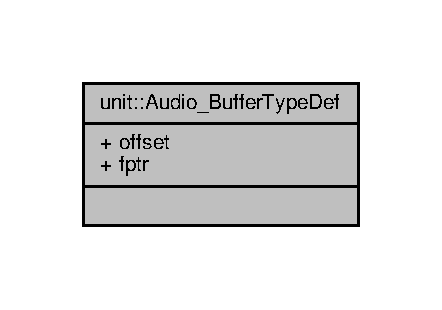
\includegraphics[width=212pt]{structunit_1_1_audio___buffer_type_def__coll__graph}
\end{center}
\end{figure}
\subsection*{Открытые атрибуты}
\begin{DoxyCompactItemize}
\item 
\mbox{\Hypertarget{structunit_1_1_audio___buffer_type_def_aec4ee0262213c87297e7aa1cc53a5f0d}\label{structunit_1_1_audio___buffer_type_def_aec4ee0262213c87297e7aa1cc53a5f0d}} 
int32\+\_\+t {\bfseries offset}
\item 
\mbox{\Hypertarget{structunit_1_1_audio___buffer_type_def_a425a22adcb26db8fc555341037bf7322}\label{structunit_1_1_audio___buffer_type_def_a425a22adcb26db8fc555341037bf7322}} 
uint32\+\_\+t {\bfseries fptr}
\end{DoxyCompactItemize}


\subsection{Подробное описание}
\begin{quote}
Задержка начала записи для устранения посторонних звуков \end{quote}


Заголовок аудио-\/файла фомата .W\+AV 

Объявления и описания членов структуры находятся в файле\+:\begin{DoxyCompactItemize}
\item 
Core/cpp/T\+Audio.\+hpp\end{DoxyCompactItemize}

\hypertarget{classapp_1_1_t_application}{}\section{Класс app\+:\+:T\+Application}
\label{classapp_1_1_t_application}\index{app\+::\+T\+Application@{app\+::\+T\+Application}}


Класс содержащий данные для обеспечения работы приложения  




{\ttfamily \#include $<$T\+Application.\+hpp$>$}



Граф связей класса app\+:\+:T\+Application\+:\nopagebreak
\begin{figure}[H]
\begin{center}
\leavevmode
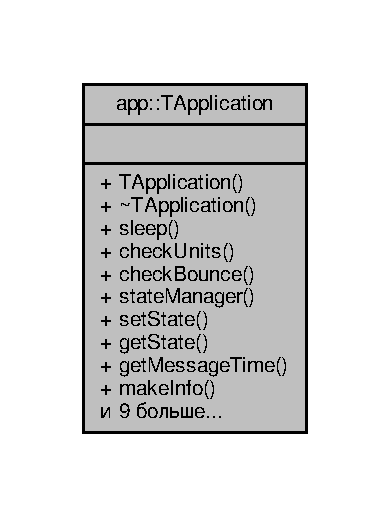
\includegraphics[width=187pt]{classapp_1_1_t_application__coll__graph}
\end{center}
\end{figure}
\subsection*{Открытые члены}
\begin{DoxyCompactItemize}
\item 
\mbox{\Hypertarget{classapp_1_1_t_application_ae9d037b0e6ebc6c26cd390ae9f5ff706}\label{classapp_1_1_t_application_ae9d037b0e6ebc6c26cd390ae9f5ff706}} 
\hyperlink{classapp_1_1_t_application_ae9d037b0e6ebc6c26cd390ae9f5ff706}{T\+Application} ()
\begin{DoxyCompactList}\small\item\em Инициализация работы приложения \end{DoxyCompactList}\item 
virtual \hyperlink{classapp_1_1_t_application_a5b7af31c95dab9a3f14ee792429a0737}{$\sim$\+T\+Application} ()
\begin{DoxyCompactList}\small\item\em По большому счёту он здесь на хрен не нужен, т.\+к. он отродясь не будет выполняться \end{DoxyCompactList}\item 
void \hyperlink{classapp_1_1_t_application_acf71a4fe338cbc1e771cc9a60431c3bf}{check\+Units} ()
\begin{DoxyCompactList}\small\item\em Тестирование устройств \end{DoxyCompactList}\item 
void \hyperlink{classapp_1_1_t_application_a4c4d1d33ea8ab73ba49a59528d200501}{check\+Bounce} ()
\begin{DoxyCompactList}\small\item\em Устранение дребезга контактов и проверка сработавшей кнопки \end{DoxyCompactList}\item 
\mbox{\Hypertarget{classapp_1_1_t_application_ae673484375cccb05d53f9f4cbeeba985}\label{classapp_1_1_t_application_ae673484375cccb05d53f9f4cbeeba985}} 
void \hyperlink{classapp_1_1_t_application_ae673484375cccb05d53f9f4cbeeba985}{state\+Manager} ()
\begin{DoxyCompactList}\small\item\em Менеджер обработки состояний \end{DoxyCompactList}\item 
bool \hyperlink{classapp_1_1_t_application_a3df1835103a3ba338821c27ad05f9f8d}{set\+State} (\hyperlink{group___xD0_x9F_xD0_xB5_xD1_x80_xD0_xB5_xD1_x87_xD0_xB8_xD1_x81_xD0_xBB_xD0_xB5_xD0_xBD_xD0_xB8_xD1_x8F_ga290e8080c661e52c2f685fd4af148acf}{app\+::app\+State})
\begin{DoxyCompactList}\small\item\em Установка состояния приложения \end{DoxyCompactList}\item 
std\+::pair$<$ \hyperlink{group___xD0_x9F_xD0_xB5_xD1_x80_xD0_xB5_xD1_x87_xD0_xB8_xD1_x81_xD0_xBB_xD0_xB5_xD0_xBD_xD0_xB8_xD1_x8F_ga290e8080c661e52c2f685fd4af148acf}{app\+::app\+State}, uint32\+\_\+t $>$ \hyperlink{classapp_1_1_t_application_a254728135b699d84f82a334708b1fbda}{get\+State} ()
\begin{DoxyCompactList}\small\item\em Получение состояния приложения \end{DoxyCompactList}\item 
std\+::string \hyperlink{classapp_1_1_t_application_aa2cb4a923a937f1a47a28fb5efe3b943}{get\+Message\+Time} ()
\begin{DoxyCompactList}\small\item\em Получить текстовое сообщение текущего времени \end{DoxyCompactList}\item 
void \hyperlink{classapp_1_1_t_application_ad6812ead3b88d21dc886d5e4d3bbfaab}{make\+Info} (const \hyperlink{group___xD0_x9F_xD0_xB5_xD1_x80_xD0_xB5_xD1_x87_xD0_xB8_xD1_x81_xD0_xBB_xD0_xB5_xD0_xBD_xD0_xB8_xD1_x8F_gaf2797b8ed91d66a25b1b3b05ea7bcfc2}{app\+::type\+Info}, const \hyperlink{group___xD0_x9F_xD0_xB5_xD1_x80_xD0_xB5_xD1_x87_xD0_xB8_xD1_x81_xD0_xBB_xD0_xB5_xD0_xBD_xD0_xB8_xD1_x8F_ga33d8f1a04a907b6c65c5dfc88280ac6f}{app\+::type\+Sound}, const uint32\+\_\+t)
\begin{DoxyCompactList}\small\item\em Управление информационными сигналом \end{DoxyCompactList}\item 
void \hyperlink{classapp_1_1_t_application_a2ac87a63360e7974afe2249f7b7e54cd}{debug\+Mesage} (const std\+::string \&)
\begin{DoxyCompactList}\small\item\em Отправка текстового отладочного сообщения \end{DoxyCompactList}\item 
void \hyperlink{classapp_1_1_t_application_a136a0f8acf017467e50018c00bad3d24}{debug\+Mesage} (const char $\ast$, const std\+::size\+\_\+t)
\begin{DoxyCompactList}\small\item\em Отправка отладочного сообщения \end{DoxyCompactList}\item 
void \hyperlink{classapp_1_1_t_application_a0c44fe0e56bc2d85720155880c9b54a6}{debug\+Mesage} (const uint8\+\_\+t $\ast$, const std\+::size\+\_\+t)
\begin{DoxyCompactList}\small\item\em Отправка цифр \end{DoxyCompactList}\item 
void \hyperlink{classapp_1_1_t_application_af84d71d883cf0745649afe65d70d290c}{debug\+Mesage} (const \hyperlink{group___xD0_x9F_xD0_xB5_xD1_x80_xD0_xB5_xD1_x87_xD0_xB8_xD1_x81_xD0_xBB_xD0_xB5_xD0_xBD_xD0_xB8_xD1_x8F_ga290e8080c661e52c2f685fd4af148acf}{app\+State})
\begin{DoxyCompactList}\small\item\em Отправка отладочного сообщения для указанного состояния \end{DoxyCompactList}\item 
\mbox{\Hypertarget{classapp_1_1_t_application_a584149b4858ba39e49970f0031689ba7}\label{classapp_1_1_t_application_a584149b4858ba39e49970f0031689ba7}} 
void \hyperlink{classapp_1_1_t_application_a584149b4858ba39e49970f0031689ba7}{debug\+Mesage} ()
\begin{DoxyCompactList}\small\item\em Отправка отладочного сообщения для текущего состояния \end{DoxyCompactList}\item 
\mbox{\Hypertarget{classapp_1_1_t_application_a2976114a4d6cb5ae83b28459e7a2aa70}\label{classapp_1_1_t_application_a2976114a4d6cb5ae83b28459e7a2aa70}} 
void \hyperlink{classapp_1_1_t_application_a2976114a4d6cb5ae83b28459e7a2aa70}{write\+Photo} ()
\begin{DoxyCompactList}\small\item\em Записываем фотку на SD\textquotesingle{}шку \end{DoxyCompactList}\end{DoxyCompactItemize}


\subsection{Подробное описание}
Класс содержащий данные для обеспечения работы приложения 

\begin{DoxyAttention}{Внимание}
Т.\+к. я пока понятия не имея как работать со временем то раз в 50 дней устройство нужно перезапускать (хотя у нас есть режим Stand\+By, а это считай перезапуск) 

Т.\+к. основной режим контроллера Stand\+By, то все указатели всегда освободятся при переходе в этот режим и выключать устройства нужно в деструкторе классов. 
\end{DoxyAttention}


\subsection{Конструктор(ы)}
\mbox{\Hypertarget{classapp_1_1_t_application_a5b7af31c95dab9a3f14ee792429a0737}\label{classapp_1_1_t_application_a5b7af31c95dab9a3f14ee792429a0737}} 
\index{app\+::\+T\+Application@{app\+::\+T\+Application}!````~T\+Application@{$\sim$\+T\+Application}}
\index{````~T\+Application@{$\sim$\+T\+Application}!app\+::\+T\+Application@{app\+::\+T\+Application}}
\subsubsection{\texorpdfstring{$\sim$\+T\+Application()}{~TApplication()}}
{\footnotesize\ttfamily app\+::\+T\+Application\+::$\sim$\+T\+Application (\begin{DoxyParamCaption}{ }\end{DoxyParamCaption})\hspace{0.3cm}{\ttfamily [virtual]}}



По большому счёту он здесь на хрен не нужен, т.\+к. он отродясь не будет выполняться 



 

\subsection{Методы}
\mbox{\Hypertarget{classapp_1_1_t_application_a4c4d1d33ea8ab73ba49a59528d200501}\label{classapp_1_1_t_application_a4c4d1d33ea8ab73ba49a59528d200501}} 
\index{app\+::\+T\+Application@{app\+::\+T\+Application}!check\+Bounce@{check\+Bounce}}
\index{check\+Bounce@{check\+Bounce}!app\+::\+T\+Application@{app\+::\+T\+Application}}
\subsubsection{\texorpdfstring{check\+Bounce()}{checkBounce()}}
{\footnotesize\ttfamily void app\+::\+T\+Application\+::check\+Bounce (\begin{DoxyParamCaption}{ }\end{DoxyParamCaption})}



Устранение дребезга контактов и проверка сработавшей кнопки 

\begin{DoxyAttention}{Внимание}
Данный запускается в обработчике прерывания и поэтому не фиг споли жевать. Быстренько проверяем нажатые кнопки и завершаем выполнение 
\end{DoxyAttention}
Граф вызовов\+:\nopagebreak
\begin{figure}[H]
\begin{center}
\leavevmode
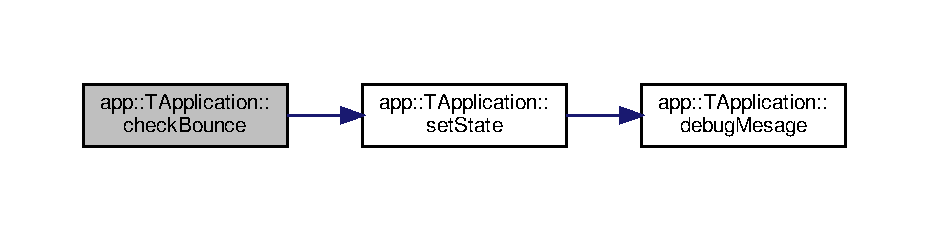
\includegraphics[width=350pt]{classapp_1_1_t_application_a4c4d1d33ea8ab73ba49a59528d200501_cgraph}
\end{center}
\end{figure}
\mbox{\Hypertarget{classapp_1_1_t_application_acf71a4fe338cbc1e771cc9a60431c3bf}\label{classapp_1_1_t_application_acf71a4fe338cbc1e771cc9a60431c3bf}} 
\index{app\+::\+T\+Application@{app\+::\+T\+Application}!check\+Units@{check\+Units}}
\index{check\+Units@{check\+Units}!app\+::\+T\+Application@{app\+::\+T\+Application}}
\subsubsection{\texorpdfstring{check\+Units()}{checkUnits()}}
{\footnotesize\ttfamily void app\+::\+T\+Application\+::check\+Units (\begin{DoxyParamCaption}{ }\end{DoxyParamCaption})}



Тестирование устройств 

Проверка периферийного оборудование. Выполняется при запуске устройства и при снятии с док станции. \begin{DoxyAttention}{Внимание}
После вызова этого метода, все периферийные устройства будут размонтированы и поэтому ОБЯЗАТЕЛЬНО (!!!) нужно уходить в режим Stand\+By или инициализировать по новой 
\end{DoxyAttention}
\mbox{\Hypertarget{classapp_1_1_t_application_a2ac87a63360e7974afe2249f7b7e54cd}\label{classapp_1_1_t_application_a2ac87a63360e7974afe2249f7b7e54cd}} 
\index{app\+::\+T\+Application@{app\+::\+T\+Application}!debug\+Mesage@{debug\+Mesage}}
\index{debug\+Mesage@{debug\+Mesage}!app\+::\+T\+Application@{app\+::\+T\+Application}}
\subsubsection{\texorpdfstring{debug\+Mesage()}{debugMesage()}\hspace{0.1cm}{\footnotesize\ttfamily [1/4]}}
{\footnotesize\ttfamily void app\+::\+T\+Application\+::debug\+Mesage (\begin{DoxyParamCaption}\item[{const std\+::string \&}]{in\+Mesage }\end{DoxyParamCaption})}



Отправка текстового отладочного сообщения 


\begin{DoxyParams}{Аргументы}
{\em in\+Mesage} & Текстовая строка которую нужно вывести в отладочный порт \\
\hline
\end{DoxyParams}
\begin{DoxyRefDesc}{Необходимо сделать}
\item[\hyperlink{todo__todo000001}{Необходимо сделать}]Переделать на хрен на потоковый вывод \end{DoxyRefDesc}
Граф вызовов\+:\nopagebreak
\begin{figure}[H]
\begin{center}
\leavevmode
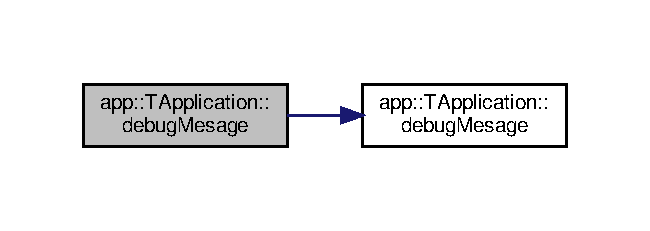
\includegraphics[width=312pt]{classapp_1_1_t_application_a2ac87a63360e7974afe2249f7b7e54cd_cgraph}
\end{center}
\end{figure}
\mbox{\Hypertarget{classapp_1_1_t_application_a136a0f8acf017467e50018c00bad3d24}\label{classapp_1_1_t_application_a136a0f8acf017467e50018c00bad3d24}} 
\index{app\+::\+T\+Application@{app\+::\+T\+Application}!debug\+Mesage@{debug\+Mesage}}
\index{debug\+Mesage@{debug\+Mesage}!app\+::\+T\+Application@{app\+::\+T\+Application}}
\subsubsection{\texorpdfstring{debug\+Mesage()}{debugMesage()}\hspace{0.1cm}{\footnotesize\ttfamily [2/4]}}
{\footnotesize\ttfamily void app\+::\+T\+Application\+::debug\+Mesage (\begin{DoxyParamCaption}\item[{const char $\ast$}]{in\+Mesage,  }\item[{const std\+::size\+\_\+t}]{in\+Size }\end{DoxyParamCaption})}



Отправка отладочного сообщения 

Данный метод выводит строку в отладочный порт 
\begin{DoxyParams}{Аргументы}
{\em in\+Mesage} & Указатель на строку, которую нужно вывести в отладочный порт \\
\hline
{\em in\+Size} & Размер выводимого бувера \\
\hline
\end{DoxyParams}
Граф вызовов\+:\nopagebreak
\begin{figure}[H]
\begin{center}
\leavevmode
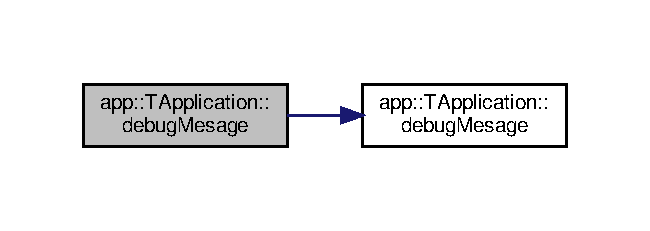
\includegraphics[width=312pt]{classapp_1_1_t_application_a136a0f8acf017467e50018c00bad3d24_cgraph}
\end{center}
\end{figure}
\mbox{\Hypertarget{classapp_1_1_t_application_a0c44fe0e56bc2d85720155880c9b54a6}\label{classapp_1_1_t_application_a0c44fe0e56bc2d85720155880c9b54a6}} 
\index{app\+::\+T\+Application@{app\+::\+T\+Application}!debug\+Mesage@{debug\+Mesage}}
\index{debug\+Mesage@{debug\+Mesage}!app\+::\+T\+Application@{app\+::\+T\+Application}}
\subsubsection{\texorpdfstring{debug\+Mesage()}{debugMesage()}\hspace{0.1cm}{\footnotesize\ttfamily [3/4]}}
{\footnotesize\ttfamily void app\+::\+T\+Application\+::debug\+Mesage (\begin{DoxyParamCaption}\item[{const uint8\+\_\+t $\ast$}]{in\+Mesage,  }\item[{const std\+::size\+\_\+t}]{in\+Size }\end{DoxyParamCaption})}



Отправка цифр 



 
\begin{DoxyParams}{Аргументы}
{\em in\+Mesage} & Указатель на массив, который нужно вывести в отладочный порт \\
\hline
{\em in\+Size} & Размер выводимого бувера \\
\hline
\end{DoxyParams}
\begin{DoxyRefDesc}{Необходимо сделать}
\item[\hyperlink{todo__todo000002}{Необходимо сделать}]Переделать на хрен на потоковый вывод \end{DoxyRefDesc}
\begin{DoxyAttention}{Внимание}
На хрена я приделал callback я понятия не имею \+:( 
\end{DoxyAttention}
\mbox{\Hypertarget{classapp_1_1_t_application_af84d71d883cf0745649afe65d70d290c}\label{classapp_1_1_t_application_af84d71d883cf0745649afe65d70d290c}} 
\index{app\+::\+T\+Application@{app\+::\+T\+Application}!debug\+Mesage@{debug\+Mesage}}
\index{debug\+Mesage@{debug\+Mesage}!app\+::\+T\+Application@{app\+::\+T\+Application}}
\subsubsection{\texorpdfstring{debug\+Mesage()}{debugMesage()}\hspace{0.1cm}{\footnotesize\ttfamily [4/4]}}
{\footnotesize\ttfamily void app\+::\+T\+Application\+::debug\+Mesage (\begin{DoxyParamCaption}\item[{const \hyperlink{group___xD0_x9F_xD0_xB5_xD1_x80_xD0_xB5_xD1_x87_xD0_xB8_xD1_x81_xD0_xBB_xD0_xB5_xD0_xBD_xD0_xB8_xD1_x8F_ga290e8080c661e52c2f685fd4af148acf}{app\+State}}]{in\+State }\end{DoxyParamCaption})}



Отправка отладочного сообщения для указанного состояния 


\begin{DoxyParams}{Аргументы}
{\em in\+State} & Состояние из app\+State \\
\hline
\end{DoxyParams}
Граф вызовов\+:\nopagebreak
\begin{figure}[H]
\begin{center}
\leavevmode
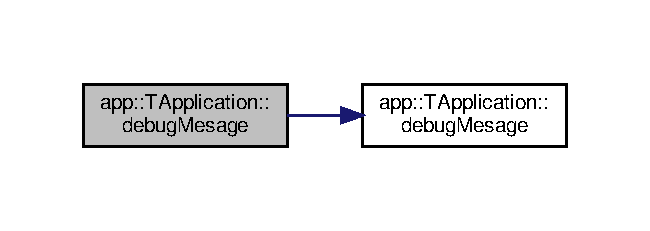
\includegraphics[width=312pt]{classapp_1_1_t_application_af84d71d883cf0745649afe65d70d290c_cgraph}
\end{center}
\end{figure}
\mbox{\Hypertarget{classapp_1_1_t_application_aa2cb4a923a937f1a47a28fb5efe3b943}\label{classapp_1_1_t_application_aa2cb4a923a937f1a47a28fb5efe3b943}} 
\index{app\+::\+T\+Application@{app\+::\+T\+Application}!get\+Message\+Time@{get\+Message\+Time}}
\index{get\+Message\+Time@{get\+Message\+Time}!app\+::\+T\+Application@{app\+::\+T\+Application}}
\subsubsection{\texorpdfstring{get\+Message\+Time()}{getMessageTime()}}
{\footnotesize\ttfamily std\+::string app\+::\+T\+Application\+::get\+Message\+Time (\begin{DoxyParamCaption}{ }\end{DoxyParamCaption})}



Получить текстовое сообщение текущего времени 

\begin{DoxyReturn}{Возвращает}
Возврат строки с текущими датой и временем 
\end{DoxyReturn}
\mbox{\Hypertarget{classapp_1_1_t_application_a254728135b699d84f82a334708b1fbda}\label{classapp_1_1_t_application_a254728135b699d84f82a334708b1fbda}} 
\index{app\+::\+T\+Application@{app\+::\+T\+Application}!get\+State@{get\+State}}
\index{get\+State@{get\+State}!app\+::\+T\+Application@{app\+::\+T\+Application}}
\subsubsection{\texorpdfstring{get\+State()}{getState()}}
{\footnotesize\ttfamily std\+::pair$<$ \hyperlink{group___xD0_x9F_xD0_xB5_xD1_x80_xD0_xB5_xD1_x87_xD0_xB8_xD1_x81_xD0_xBB_xD0_xB5_xD0_xBD_xD0_xB8_xD1_x8F_ga290e8080c661e52c2f685fd4af148acf}{app\+::app\+State}, uint32\+\_\+t $>$ app\+::\+T\+Application\+::get\+State (\begin{DoxyParamCaption}{ }\end{DoxyParamCaption})}



Получение состояния приложения 

\begin{DoxyReturn}{Возвращает}
пара -\/ Текущее состояние и продолжительность данного состояния 
\end{DoxyReturn}
\mbox{\Hypertarget{classapp_1_1_t_application_ad6812ead3b88d21dc886d5e4d3bbfaab}\label{classapp_1_1_t_application_ad6812ead3b88d21dc886d5e4d3bbfaab}} 
\index{app\+::\+T\+Application@{app\+::\+T\+Application}!make\+Info@{make\+Info}}
\index{make\+Info@{make\+Info}!app\+::\+T\+Application@{app\+::\+T\+Application}}
\subsubsection{\texorpdfstring{make\+Info()}{makeInfo()}}
{\footnotesize\ttfamily void app\+::\+T\+Application\+::make\+Info (\begin{DoxyParamCaption}\item[{const \hyperlink{group___xD0_x9F_xD0_xB5_xD1_x80_xD0_xB5_xD1_x87_xD0_xB8_xD1_x81_xD0_xBB_xD0_xB5_xD0_xBD_xD0_xB8_xD1_x8F_gaf2797b8ed91d66a25b1b3b05ea7bcfc2}{app\+::type\+Info}}]{in\+Type\+Info,  }\item[{const \hyperlink{group___xD0_x9F_xD0_xB5_xD1_x80_xD0_xB5_xD1_x87_xD0_xB8_xD1_x81_xD0_xBB_xD0_xB5_xD0_xBD_xD0_xB8_xD1_x8F_ga33d8f1a04a907b6c65c5dfc88280ac6f}{app\+::type\+Sound}}]{in\+Type\+Sound,  }\item[{const uint32\+\_\+t}]{in\+Duration }\end{DoxyParamCaption})}



Управление информационными сигналом 

Включение пищалки и звука Если продолжительность звучания равна 0, то сигнал будет звучать непрерывно и прервать его будет нельзя. Если продолжительность звучания меньше 100, то измеряется в количестве пиков (максимально 99) 
\begin{DoxyParams}{Аргументы}
{\em in\+Type\+Sound} & Тип звукового сигнала \\
\hline
{\em in\+Duration} & Продолжительность в милисекундах. Если = 0, то сигнал звучит непрерывно. \\
\hline
\end{DoxyParams}
\mbox{\Hypertarget{classapp_1_1_t_application_a3df1835103a3ba338821c27ad05f9f8d}\label{classapp_1_1_t_application_a3df1835103a3ba338821c27ad05f9f8d}} 
\index{app\+::\+T\+Application@{app\+::\+T\+Application}!set\+State@{set\+State}}
\index{set\+State@{set\+State}!app\+::\+T\+Application@{app\+::\+T\+Application}}
\subsubsection{\texorpdfstring{set\+State()}{setState()}}
{\footnotesize\ttfamily bool app\+::\+T\+Application\+::set\+State (\begin{DoxyParamCaption}\item[{\hyperlink{group___xD0_x9F_xD0_xB5_xD1_x80_xD0_xB5_xD1_x87_xD0_xB8_xD1_x81_xD0_xBB_xD0_xB5_xD0_xBD_xD0_xB8_xD1_x8F_ga290e8080c661e52c2f685fd4af148acf}{app\+::app\+State}}]{in\+App\+State }\end{DoxyParamCaption})}



Установка состояния приложения 


\begin{DoxyParams}{Аргументы}
{\em in\+App\+State} & \\
\hline
\end{DoxyParams}
\begin{DoxyReturn}{Возвращает}
При успешной установке статуса возвращается true 
\end{DoxyReturn}
\begin{DoxyAttention}{Внимание}
Возврат может пригодиться в будущем, если вдруг будет учитываться допустимость перехода состояний 
\end{DoxyAttention}
Граф вызовов\+:\nopagebreak
\begin{figure}[H]
\begin{center}
\leavevmode
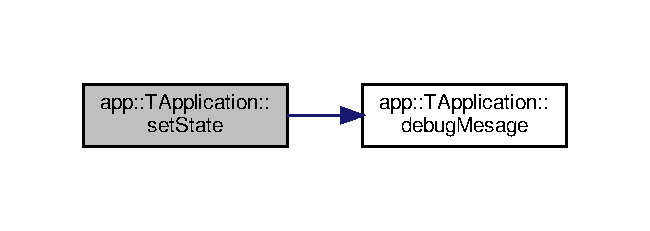
\includegraphics[width=312pt]{classapp_1_1_t_application_a3df1835103a3ba338821c27ad05f9f8d_cgraph}
\end{center}
\end{figure}


Объявления и описания членов классов находятся в файлах\+:\begin{DoxyCompactItemize}
\item 
Core/cpp/T\+Application.\+hpp\item 
Core/cpp/T\+Application.\+cpp\end{DoxyCompactItemize}

\hypertarget{classunit_1_1_t_audio}{}\section{Класс unit\+:\+:T\+Audio}
\label{classunit_1_1_t_audio}\index{unit\+::\+T\+Audio@{unit\+::\+T\+Audio}}


{\ttfamily \#include $<$T\+Audio.\+hpp$>$}



Граф наследования\+:unit\+:\+:T\+Audio\+:\nopagebreak
\begin{figure}[H]
\begin{center}
\leavevmode
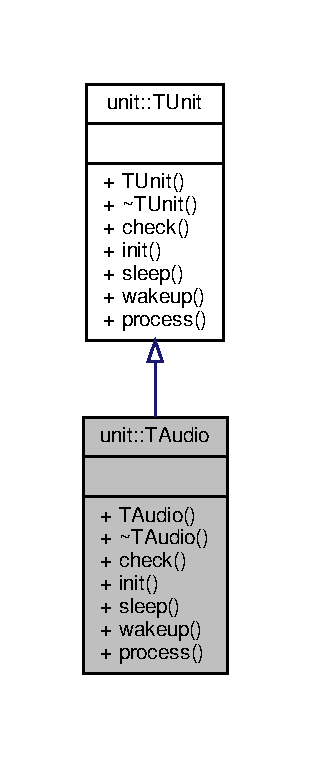
\includegraphics[width=149pt]{classunit_1_1_t_audio__inherit__graph}
\end{center}
\end{figure}


Граф связей класса unit\+:\+:T\+Audio\+:\nopagebreak
\begin{figure}[H]
\begin{center}
\leavevmode
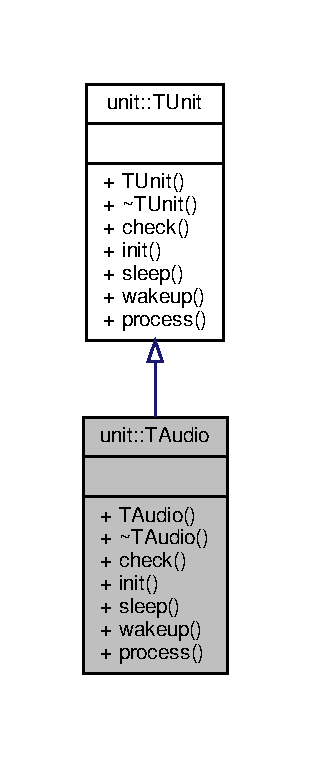
\includegraphics[width=149pt]{classunit_1_1_t_audio__coll__graph}
\end{center}
\end{figure}
\subsection*{Открытые члены}
\begin{DoxyCompactItemize}
\item 
\hyperlink{classunit_1_1_t_audio_a326d9d807df56ef1a264564c69c350b5}{T\+Audio} (std\+::shared\+\_\+ptr$<$ \hyperlink{classunit_1_1_t_file_system}{T\+File\+System} $>$)
\item 
virtual \hyperlink{classunit_1_1_t_audio_ab62b7453a3128fd1ab9d2473237ba331}{$\sim$\+T\+Audio} ()
\item 
\mbox{\Hypertarget{classunit_1_1_t_audio_a69cc926edc98c59e9ffaad10ceb605f0}\label{classunit_1_1_t_audio_a69cc926edc98c59e9ffaad10ceb605f0}} 
bool \hyperlink{classunit_1_1_t_audio_a69cc926edc98c59e9ffaad10ceb605f0}{check} ()
\begin{DoxyCompactList}\small\item\em Проверка работоспособности аудио (запись и вопроизведение пищалки) \end{DoxyCompactList}\item 
\mbox{\Hypertarget{classunit_1_1_t_audio_a362d211c87c2497e12792243cc2c0fc9}\label{classunit_1_1_t_audio_a362d211c87c2497e12792243cc2c0fc9}} 
void \hyperlink{classunit_1_1_t_audio_a362d211c87c2497e12792243cc2c0fc9}{init} ()
\begin{DoxyCompactList}\small\item\em Инициализация устройства \end{DoxyCompactList}\item 
\mbox{\Hypertarget{classunit_1_1_t_audio_aab519e5239080d5ef906293dedc9399a}\label{classunit_1_1_t_audio_aab519e5239080d5ef906293dedc9399a}} 
void \hyperlink{classunit_1_1_t_audio_aab519e5239080d5ef906293dedc9399a}{sleep} ()
\begin{DoxyCompactList}\small\item\em Перевод в режим энергосбережения \end{DoxyCompactList}\item 
\mbox{\Hypertarget{classunit_1_1_t_audio_a3cbc7de5ae0d03af42eeed896829d85c}\label{classunit_1_1_t_audio_a3cbc7de5ae0d03af42eeed896829d85c}} 
void \hyperlink{classunit_1_1_t_audio_a3cbc7de5ae0d03af42eeed896829d85c}{wakeup} ()
\begin{DoxyCompactList}\small\item\em Выход из режима энергосбережения \end{DoxyCompactList}\item 
bool \hyperlink{classunit_1_1_t_audio_ad547ef4d28534b9cd76d2e7eb539d1e0}{process} ()
\begin{DoxyCompactList}\small\item\em Получение данных с микрофона и запись его в файл \end{DoxyCompactList}\end{DoxyCompactItemize}


\subsection{Подробное описание}


 Класс для работы со звуком Запись звука идёт в буфер по D\+MA и по срабатываний прерываний выполняется преобразование из P\+DM в P\+CM запись результата на SD 

\subsection{Конструктор(ы)}
\mbox{\Hypertarget{classunit_1_1_t_audio_a326d9d807df56ef1a264564c69c350b5}\label{classunit_1_1_t_audio_a326d9d807df56ef1a264564c69c350b5}} 
\index{unit\+::\+T\+Audio@{unit\+::\+T\+Audio}!T\+Audio@{T\+Audio}}
\index{T\+Audio@{T\+Audio}!unit\+::\+T\+Audio@{unit\+::\+T\+Audio}}
\subsubsection{\texorpdfstring{T\+Audio()}{TAudio()}}
{\footnotesize\ttfamily unit\+::\+T\+Audio\+::\+T\+Audio (\begin{DoxyParamCaption}\item[{std\+::shared\+\_\+ptr$<$ \hyperlink{classunit_1_1_t_file_system}{T\+File\+System} $>$}]{in\+Ptr\+File\+System }\end{DoxyParamCaption})}

Конструктор инициализирующий работу для записи аудио. Все данные для P\+DM -\/$>$ P\+CM преобразования задаются в настройках Cube\+MX 
\begin{DoxyParams}{Аргументы}
{\em in\+Ptr\+File\+System} & Указатель на класс работы с файловой системой \\
\hline
\end{DoxyParams}
\begin{DoxyAttention}{Внимание}
Я ни коем образом не проверяю указатель на файловую систему!!! sizeof (\hyperlink{namespacecommon_aeca12b629edac6586f4b0fbcf9617769}{common\+::st\+Audio\+Buf})/2 
\end{DoxyAttention}
\mbox{\Hypertarget{classunit_1_1_t_audio_ab62b7453a3128fd1ab9d2473237ba331}\label{classunit_1_1_t_audio_ab62b7453a3128fd1ab9d2473237ba331}} 
\index{unit\+::\+T\+Audio@{unit\+::\+T\+Audio}!````~T\+Audio@{$\sim$\+T\+Audio}}
\index{````~T\+Audio@{$\sim$\+T\+Audio}!unit\+::\+T\+Audio@{unit\+::\+T\+Audio}}
\subsubsection{\texorpdfstring{$\sim$\+T\+Audio()}{~TAudio()}}
{\footnotesize\ttfamily unit\+::\+T\+Audio\+::$\sim$\+T\+Audio (\begin{DoxyParamCaption}{ }\end{DoxyParamCaption})\hspace{0.3cm}{\ttfamily [virtual]}}

\begin{DoxyAttention}{Внимание}
По хорошему нужно проверять и дожидаться остановки D\+MA, т.\+к. в противном случае контроллер не уйдёт в Stand\+By 
\end{DoxyAttention}


\subsection{Методы}
\mbox{\Hypertarget{classunit_1_1_t_audio_ad547ef4d28534b9cd76d2e7eb539d1e0}\label{classunit_1_1_t_audio_ad547ef4d28534b9cd76d2e7eb539d1e0}} 
\index{unit\+::\+T\+Audio@{unit\+::\+T\+Audio}!process@{process}}
\index{process@{process}!unit\+::\+T\+Audio@{unit\+::\+T\+Audio}}
\subsubsection{\texorpdfstring{process()}{process()}}
{\footnotesize\ttfamily bool unit\+::\+T\+Audio\+::process (\begin{DoxyParamCaption}{ }\end{DoxyParamCaption})\hspace{0.3cm}{\ttfamily [virtual]}}



Получение данных с микрофона и запись его в файл 



 Запись буфера полученного с микрофона \begin{DoxyReturn}{Возвращает}
true в случае успешной записи 
\end{DoxyReturn}
\begin{DoxyRefDesc}{Необходимо сделать}
\item[\hyperlink{todo__todo000005}{Необходимо сделать}]Переделать на хрен, т.\+к. написано через жопу кривыми руками. \+:( \end{DoxyRefDesc}


Замещает \hyperlink{classunit_1_1_t_unit_a108691c8b988d97c65237c83a31db706}{unit\+::\+T\+Unit}.



Объявления и описания членов классов находятся в файлах\+:\begin{DoxyCompactItemize}
\item 
Core/cpp/T\+Audio.\+hpp\item 
Core/cpp/T\+Audio.\+cpp\end{DoxyCompactItemize}

\hypertarget{classunit_1_1_t_bq25121}{}\section{Класс unit\+:\+:T\+Bq25121}
\label{classunit_1_1_t_bq25121}\index{unit\+::\+T\+Bq25121@{unit\+::\+T\+Bq25121}}


{\ttfamily \#include $<$T\+Bq25121.\+hpp$>$}



Граф наследования\+:unit\+:\+:T\+Bq25121\+:\nopagebreak
\begin{figure}[H]
\begin{center}
\leavevmode
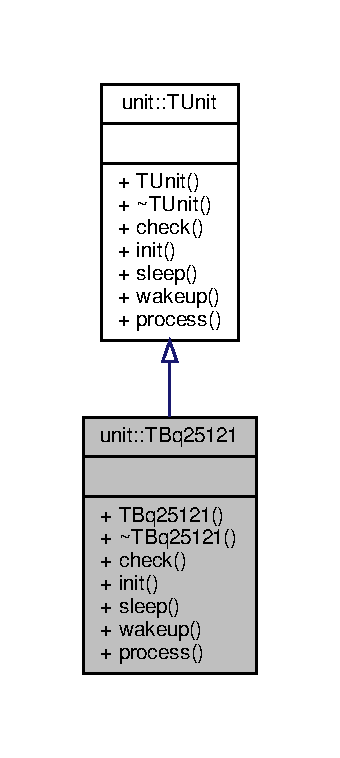
\includegraphics[width=163pt]{classunit_1_1_t_bq25121__inherit__graph}
\end{center}
\end{figure}


Граф связей класса unit\+:\+:T\+Bq25121\+:\nopagebreak
\begin{figure}[H]
\begin{center}
\leavevmode
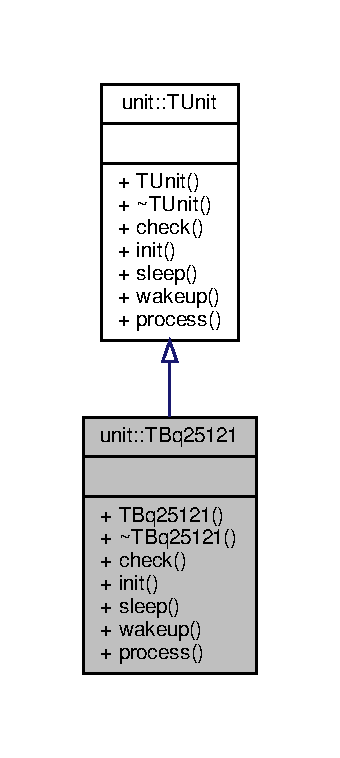
\includegraphics[width=163pt]{classunit_1_1_t_bq25121__coll__graph}
\end{center}
\end{figure}
\subsection*{Открытые члены}
\begin{DoxyCompactItemize}
\item 
\hyperlink{classunit_1_1_t_bq25121_ae620c44c80792004e5ed25182964d419}{T\+Bq25121} ()
\item 
\mbox{\Hypertarget{classunit_1_1_t_bq25121_a0971e07af4532b7cc33517cb72d1279b}\label{classunit_1_1_t_bq25121_a0971e07af4532b7cc33517cb72d1279b}} 
bool \hyperlink{classunit_1_1_t_bq25121_a0971e07af4532b7cc33517cb72d1279b}{check} ()
\begin{DoxyCompactList}\small\item\em Проверка работоспособности чипа B\+Q25121. \end{DoxyCompactList}\item 
void \hyperlink{classunit_1_1_t_bq25121_a195490b2493631c50f5f7380436c24be}{init} ()
\begin{DoxyCompactList}\small\item\em Инициализация устройства \end{DoxyCompactList}\item 
\mbox{\Hypertarget{classunit_1_1_t_bq25121_a769c16732c917f24c1b36292f13df415}\label{classunit_1_1_t_bq25121_a769c16732c917f24c1b36292f13df415}} 
void \hyperlink{classunit_1_1_t_bq25121_a769c16732c917f24c1b36292f13df415}{sleep} ()
\begin{DoxyCompactList}\small\item\em Перевод в режим энергосбережения \end{DoxyCompactList}\item 
\mbox{\Hypertarget{classunit_1_1_t_bq25121_a37ee8c808bce005ac349c0ea4ee9cf32}\label{classunit_1_1_t_bq25121_a37ee8c808bce005ac349c0ea4ee9cf32}} 
void \hyperlink{classunit_1_1_t_bq25121_a37ee8c808bce005ac349c0ea4ee9cf32}{wakeup} ()
\begin{DoxyCompactList}\small\item\em Выход из режима энергосбережения \end{DoxyCompactList}\item 
\mbox{\Hypertarget{classunit_1_1_t_bq25121_aef9b6fa9ec1e989523fa1584cb604a7d}\label{classunit_1_1_t_bq25121_aef9b6fa9ec1e989523fa1584cb604a7d}} 
bool \hyperlink{classunit_1_1_t_bq25121_aef9b6fa9ec1e989523fa1584cb604a7d}{process} ()
\begin{DoxyCompactList}\small\item\em Получение данных \end{DoxyCompactList}\end{DoxyCompactItemize}


\subsection{Подробное описание}
Класс для работы с чипом B\+Q25121 

\subsection{Конструктор(ы)}
\mbox{\Hypertarget{classunit_1_1_t_bq25121_ae620c44c80792004e5ed25182964d419}\label{classunit_1_1_t_bq25121_ae620c44c80792004e5ed25182964d419}} 
\index{unit\+::\+T\+Bq25121@{unit\+::\+T\+Bq25121}!T\+Bq25121@{T\+Bq25121}}
\index{T\+Bq25121@{T\+Bq25121}!unit\+::\+T\+Bq25121@{unit\+::\+T\+Bq25121}}
\subsubsection{\texorpdfstring{T\+Bq25121()}{TBq25121()}}
{\footnotesize\ttfamily unit\+::\+T\+Bq25121\+::\+T\+Bq25121 (\begin{DoxyParamCaption}{ }\end{DoxyParamCaption})}

В конструкторе класса всегда программируется работа чипа B\+Q25121 При возникновении ошибки будет подан сигнал Один длинный гудок и два коротких Граф вызовов\+:\nopagebreak
\begin{figure}[H]
\begin{center}
\leavevmode
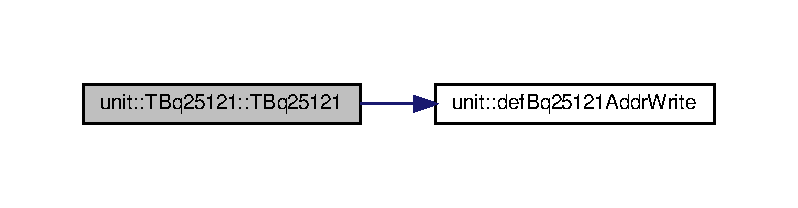
\includegraphics[width=350pt]{classunit_1_1_t_bq25121_ae620c44c80792004e5ed25182964d419_cgraph}
\end{center}
\end{figure}


\subsection{Методы}
\mbox{\Hypertarget{classunit_1_1_t_bq25121_a195490b2493631c50f5f7380436c24be}\label{classunit_1_1_t_bq25121_a195490b2493631c50f5f7380436c24be}} 
\index{unit\+::\+T\+Bq25121@{unit\+::\+T\+Bq25121}!init@{init}}
\index{init@{init}!unit\+::\+T\+Bq25121@{unit\+::\+T\+Bq25121}}
\subsubsection{\texorpdfstring{init()}{init()}}
{\footnotesize\ttfamily void unit\+::\+T\+Bq25121\+::init (\begin{DoxyParamCaption}{ }\end{DoxyParamCaption})\hspace{0.3cm}{\ttfamily [virtual]}}



Инициализация устройства 



 Полный аппаратный сброс чипа и программирование регистров 

Замещает \hyperlink{classunit_1_1_t_unit_afc001dd57ba88e571e6b650a416b76a5}{unit\+::\+T\+Unit}.

Граф вызовов\+:\nopagebreak
\begin{figure}[H]
\begin{center}
\leavevmode
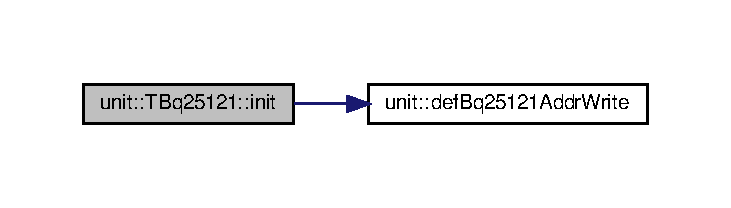
\includegraphics[width=350pt]{classunit_1_1_t_bq25121_a195490b2493631c50f5f7380436c24be_cgraph}
\end{center}
\end{figure}


Объявления и описания членов классов находятся в файлах\+:\begin{DoxyCompactItemize}
\item 
Core/cpp/T\+Bq25121.\+hpp\item 
Core/cpp/T\+Bq25121.\+cpp\end{DoxyCompactItemize}

\hypertarget{classapp_1_1_t_button}{}\section{Класс app\+:\+:T\+Button}
\label{classapp_1_1_t_button}\index{app\+::\+T\+Button@{app\+::\+T\+Button}}


Класс для работы с кнопками  




{\ttfamily \#include $<$T\+Button.\+hpp$>$}



Граф связей класса app\+:\+:T\+Button\+:\nopagebreak
\begin{figure}[H]
\begin{center}
\leavevmode
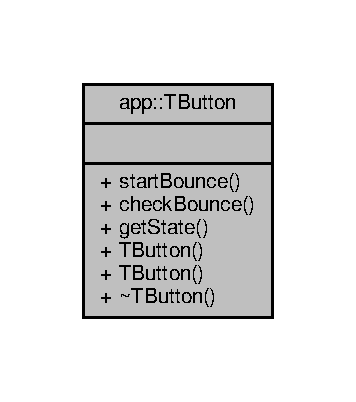
\includegraphics[width=171pt]{classapp_1_1_t_button__coll__graph}
\end{center}
\end{figure}
\subsection*{Открытые члены}
\begin{DoxyCompactItemize}
\item 
void \hyperlink{classapp_1_1_t_button_a92fc2dcb3d54a563b7b1a96900a4717c}{start\+Bounce} ()
\begin{DoxyCompactList}\small\item\em Запуск процедуры устранения дребезга \end{DoxyCompactList}\item 
bool \hyperlink{classapp_1_1_t_button_a52714fba93672ac5690de6f9d56e9a5f}{check\+Bounce} ()
\begin{DoxyCompactList}\small\item\em Проверка устранения дребезга контактов \end{DoxyCompactList}\item 
G\+P\+I\+O\+\_\+\+Pin\+State \hyperlink{classapp_1_1_t_button_a1d6cf41ee0a98746592b1d604041f8ce}{get\+State} ()
\begin{DoxyCompactList}\small\item\em Получение состояния кнопки. \end{DoxyCompactList}\item 
\hyperlink{classapp_1_1_t_button_a846432bef1a2f5f2705eef5f95d22ae2}{T\+Button} (G\+P\+I\+O\+\_\+\+Type\+Def $\ast$, uint16\+\_\+t)
\end{DoxyCompactItemize}


\subsection{Подробное описание}
Класс для работы с кнопками 

\subsection{Конструктор(ы)}
\mbox{\Hypertarget{classapp_1_1_t_button_a846432bef1a2f5f2705eef5f95d22ae2}\label{classapp_1_1_t_button_a846432bef1a2f5f2705eef5f95d22ae2}} 
\index{app\+::\+T\+Button@{app\+::\+T\+Button}!T\+Button@{T\+Button}}
\index{T\+Button@{T\+Button}!app\+::\+T\+Button@{app\+::\+T\+Button}}
\subsubsection{\texorpdfstring{T\+Button()}{TButton()}}
{\footnotesize\ttfamily app\+::\+T\+Button\+::\+T\+Button (\begin{DoxyParamCaption}\item[{G\+P\+I\+O\+\_\+\+Type\+Def $\ast$}]{in\+Gpio\+Port,  }\item[{uint16\+\_\+t}]{in\+Gpio }\end{DoxyParamCaption})}


\begin{DoxyParams}{Аргументы}
{\em in\+Gpio\+Port} & Регистр G\+P\+IO \\
\hline
{\em in\+Gpio} & Пин \\
\hline
\end{DoxyParams}
\begin{DoxyAttention}{Внимание}
Я ни коем образом не проверяю правильность передачи параметров 
\end{DoxyAttention}


\subsection{Методы}
\mbox{\Hypertarget{classapp_1_1_t_button_a52714fba93672ac5690de6f9d56e9a5f}\label{classapp_1_1_t_button_a52714fba93672ac5690de6f9d56e9a5f}} 
\index{app\+::\+T\+Button@{app\+::\+T\+Button}!check\+Bounce@{check\+Bounce}}
\index{check\+Bounce@{check\+Bounce}!app\+::\+T\+Button@{app\+::\+T\+Button}}
\subsubsection{\texorpdfstring{check\+Bounce()}{checkBounce()}}
{\footnotesize\ttfamily bool app\+::\+T\+Button\+::check\+Bounce (\begin{DoxyParamCaption}{ }\end{DoxyParamCaption})}



Проверка устранения дребезга контактов 

\begin{DoxyReturn}{Возвращает}
true Если дребезг устранен 
\end{DoxyReturn}
\mbox{\Hypertarget{classapp_1_1_t_button_a1d6cf41ee0a98746592b1d604041f8ce}\label{classapp_1_1_t_button_a1d6cf41ee0a98746592b1d604041f8ce}} 
\index{app\+::\+T\+Button@{app\+::\+T\+Button}!get\+State@{get\+State}}
\index{get\+State@{get\+State}!app\+::\+T\+Button@{app\+::\+T\+Button}}
\subsubsection{\texorpdfstring{get\+State()}{getState()}}
{\footnotesize\ttfamily G\+P\+I\+O\+\_\+\+Pin\+State app\+::\+T\+Button\+::get\+State (\begin{DoxyParamCaption}{ }\end{DoxyParamCaption})}



Получение состояния кнопки. 

\begin{DoxyReturn}{Возвращает}
Состояние нажатой кнопки. 
\end{DoxyReturn}
\begin{DoxyAttention}{Внимание}
Устранение дребезга не проверяется вообще. 
\end{DoxyAttention}
\mbox{\Hypertarget{classapp_1_1_t_button_a92fc2dcb3d54a563b7b1a96900a4717c}\label{classapp_1_1_t_button_a92fc2dcb3d54a563b7b1a96900a4717c}} 
\index{app\+::\+T\+Button@{app\+::\+T\+Button}!start\+Bounce@{start\+Bounce}}
\index{start\+Bounce@{start\+Bounce}!app\+::\+T\+Button@{app\+::\+T\+Button}}
\subsubsection{\texorpdfstring{start\+Bounce()}{startBounce()}}
{\footnotesize\ttfamily void app\+::\+T\+Button\+::start\+Bounce (\begin{DoxyParamCaption}{ }\end{DoxyParamCaption})}



Запуск процедуры устранения дребезга 

Вне зависимости от состояния тупо запускаем устранение дребезга контактов. 

Объявления и описания членов классов находятся в файлах\+:\begin{DoxyCompactItemize}
\item 
Core/cpp/T\+Button.\+hpp\item 
Core/cpp/T\+Button.\+cpp\end{DoxyCompactItemize}

\hypertarget{structapp_1_1td_log_item}{}\section{Структура app\+:\+:td\+Log\+Item}
\label{structapp_1_1td_log_item}\index{app\+::td\+Log\+Item@{app\+::td\+Log\+Item}}


Описание структуры для хранения одной записи лога.  




{\ttfamily \#include $<$T\+Log.\+hpp$>$}



Граф связей класса app\+:\+:td\+Log\+Item\+:\nopagebreak
\begin{figure}[H]
\begin{center}
\leavevmode
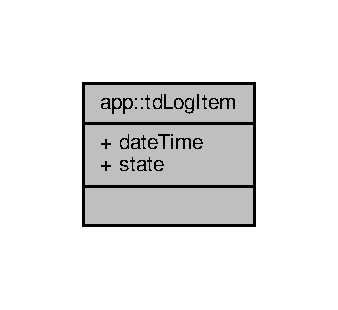
\includegraphics[width=162pt]{structapp_1_1td_log_item__coll__graph}
\end{center}
\end{figure}
\subsection*{Открытые атрибуты}
\begin{DoxyCompactItemize}
\item 
\mbox{\Hypertarget{structapp_1_1td_log_item_a5cb3959fafb84783a88a840f8427e4e6}\label{structapp_1_1td_log_item_a5cb3959fafb84783a88a840f8427e4e6}} 
uint32\+\_\+t \hyperlink{structapp_1_1td_log_item_a5cb3959fafb84783a88a840f8427e4e6}{date\+Time}
\begin{DoxyCompactList}\small\item\em Дата время события с точностью до двух сек. \end{DoxyCompactList}\item 
\mbox{\Hypertarget{structapp_1_1td_log_item_ade62dcc4582ad2247c47a3e68889d118}\label{structapp_1_1td_log_item_ade62dcc4582ad2247c47a3e68889d118}} 
\hyperlink{namespaceapp_a290e8080c661e52c2f685fd4af148acf}{app\+::app\+State} \hyperlink{structapp_1_1td_log_item_ade62dcc4582ad2247c47a3e68889d118}{state}
\begin{DoxyCompactList}\small\item\em Состояние события \end{DoxyCompactList}\end{DoxyCompactItemize}


\subsection{Подробное описание}
Описание структуры для хранения одной записи лога. 

Объявления и описания членов структуры находятся в файле\+:\begin{DoxyCompactItemize}
\item 
Core/cpp/T\+Log.\+hpp\end{DoxyCompactItemize}

\hypertarget{classunit_1_1_t_file_system}{}\section{Класс unit\+:\+:T\+File\+System}
\label{classunit_1_1_t_file_system}\index{unit\+::\+T\+File\+System@{unit\+::\+T\+File\+System}}


Класс для работы с файловой системой  




{\ttfamily \#include $<$T\+File\+System.\+hpp$>$}



Граф наследования\+:unit\+:\+:T\+File\+System\+:\nopagebreak
\begin{figure}[H]
\begin{center}
\leavevmode
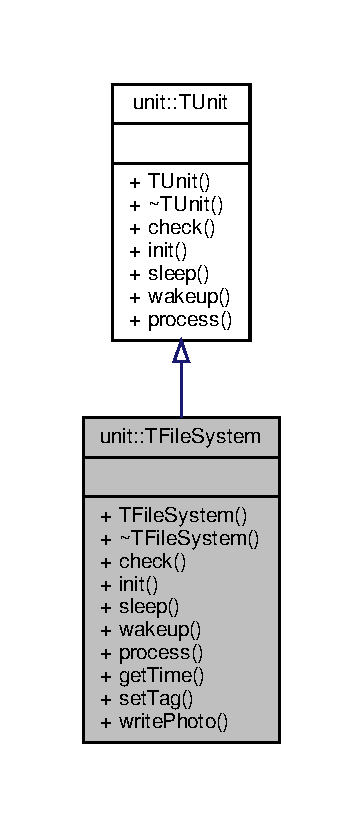
\includegraphics[width=174pt]{classunit_1_1_t_file_system__inherit__graph}
\end{center}
\end{figure}


Граф связей класса unit\+:\+:T\+File\+System\+:\nopagebreak
\begin{figure}[H]
\begin{center}
\leavevmode
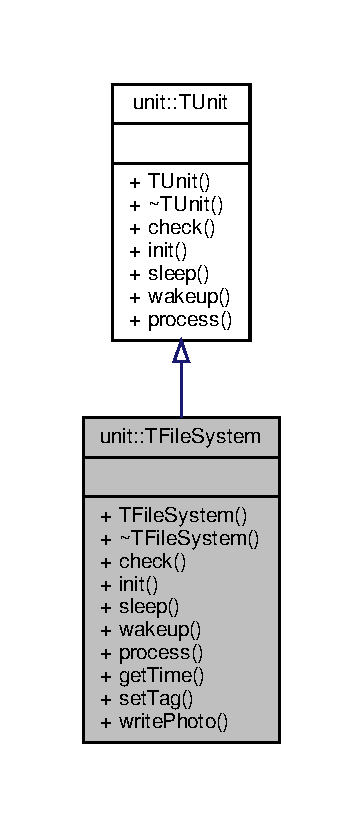
\includegraphics[width=174pt]{classunit_1_1_t_file_system__coll__graph}
\end{center}
\end{figure}
\subsection*{Открытые члены}
\begin{DoxyCompactItemize}
\item 
\hyperlink{classunit_1_1_t_file_system_ac45162c4d69b6661aab204724af57322}{T\+File\+System} ()
\item 
virtual \hyperlink{classunit_1_1_t_file_system_a87299dbbdea872b06972f1432ef9ef88}{$\sim$\+T\+File\+System} ()
\item 
bool \hyperlink{classunit_1_1_t_file_system_a0737b50d219570ae2e11ea17a32cc85c}{check} ()
\begin{DoxyCompactList}\small\item\em Проверка работоспособности S\+D-\/карточки \end{DoxyCompactList}\item 
\mbox{\Hypertarget{classunit_1_1_t_file_system_a036085cc2f2674f9ea89426000b6ba02}\label{classunit_1_1_t_file_system_a036085cc2f2674f9ea89426000b6ba02}} 
void \hyperlink{classunit_1_1_t_file_system_a036085cc2f2674f9ea89426000b6ba02}{init} ()
\begin{DoxyCompactList}\small\item\em Инициализация устройства \end{DoxyCompactList}\item 
\mbox{\Hypertarget{classunit_1_1_t_file_system_a4e4fd801d58a5c6b526a65ec5cb187dd}\label{classunit_1_1_t_file_system_a4e4fd801d58a5c6b526a65ec5cb187dd}} 
void \hyperlink{classunit_1_1_t_file_system_a4e4fd801d58a5c6b526a65ec5cb187dd}{sleep} ()
\begin{DoxyCompactList}\small\item\em Перевод в режим энергосбережения \end{DoxyCompactList}\item 
\mbox{\Hypertarget{classunit_1_1_t_file_system_a99d5e06aee69d3674ea441f140f6a47b}\label{classunit_1_1_t_file_system_a99d5e06aee69d3674ea441f140f6a47b}} 
void \hyperlink{classunit_1_1_t_file_system_a99d5e06aee69d3674ea441f140f6a47b}{wakeup} ()
\begin{DoxyCompactList}\small\item\em Выход из режима энергосбережения \end{DoxyCompactList}\item 
\mbox{\Hypertarget{classunit_1_1_t_file_system_af7969ea11284d9f6f093687f0ba90082}\label{classunit_1_1_t_file_system_af7969ea11284d9f6f093687f0ba90082}} 
bool \hyperlink{classunit_1_1_t_file_system_af7969ea11284d9f6f093687f0ba90082}{process} ()
\begin{DoxyCompactList}\small\item\em Получение данных \end{DoxyCompactList}\item 
void \hyperlink{classunit_1_1_t_file_system_aaf4766a6f4dcd6759e362ffc977615f5}{get\+Time} ()
\begin{DoxyCompactList}\small\item\em Синхронизация времени \end{DoxyCompactList}\item 
void \hyperlink{classunit_1_1_t_file_system_a79523b2edca3574ec6254af671f28256}{set\+Tag} ()
\begin{DoxyCompactList}\small\item\em Запись на SD ID сосканированной метки \end{DoxyCompactList}\item 
\mbox{\Hypertarget{classunit_1_1_t_file_system_aacd7aae1827432b04c06b9a1d440b949}\label{classunit_1_1_t_file_system_aacd7aae1827432b04c06b9a1d440b949}} 
bool \hyperlink{classunit_1_1_t_file_system_aacd7aae1827432b04c06b9a1d440b949}{write\+Photo} ()
\begin{DoxyCompactList}\small\item\em Запись на SD изображения полученного с камеры \end{DoxyCompactList}\end{DoxyCompactItemize}


\subsection{Подробное описание}
Класс для работы с файловой системой 

Класс для работы с файловой системой на S\+D-\/карточке. Он нужен только что-\/бы записывать туда фотки, аудио и метки. \begin{DoxyAttention}{Внимание}
Перед работой с файловой системой всегда необходимо инициальзировать SD карточку 
\end{DoxyAttention}


\subsection{Конструктор(ы)}
\mbox{\Hypertarget{classunit_1_1_t_file_system_ac45162c4d69b6661aab204724af57322}\label{classunit_1_1_t_file_system_ac45162c4d69b6661aab204724af57322}} 
\index{unit\+::\+T\+File\+System@{unit\+::\+T\+File\+System}!T\+File\+System@{T\+File\+System}}
\index{T\+File\+System@{T\+File\+System}!unit\+::\+T\+File\+System@{unit\+::\+T\+File\+System}}
\subsubsection{\texorpdfstring{T\+File\+System()}{TFileSystem()}}
{\footnotesize\ttfamily unit\+::\+T\+File\+System\+::\+T\+File\+System (\begin{DoxyParamCaption}{ }\end{DoxyParamCaption})}

Монтируем файловую систему. \begin{DoxyAttention}{Внимание}
SD карта должна быть уже проинициализированна 
\end{DoxyAttention}
\mbox{\Hypertarget{classunit_1_1_t_file_system_a87299dbbdea872b06972f1432ef9ef88}\label{classunit_1_1_t_file_system_a87299dbbdea872b06972f1432ef9ef88}} 
\index{unit\+::\+T\+File\+System@{unit\+::\+T\+File\+System}!````~T\+File\+System@{$\sim$\+T\+File\+System}}
\index{````~T\+File\+System@{$\sim$\+T\+File\+System}!unit\+::\+T\+File\+System@{unit\+::\+T\+File\+System}}
\subsubsection{\texorpdfstring{$\sim$\+T\+File\+System()}{~TFileSystem()}}
{\footnotesize\ttfamily unit\+::\+T\+File\+System\+::$\sim$\+T\+File\+System (\begin{DoxyParamCaption}{ }\end{DoxyParamCaption})\hspace{0.3cm}{\ttfamily [virtual]}}

\begin{DoxyAttention}{Внимание}
Файловая система должна быть размонтирована всегда, в противном случае SD\textquotesingle{}шка убивается 
\end{DoxyAttention}


\subsection{Методы}
\mbox{\Hypertarget{classunit_1_1_t_file_system_a0737b50d219570ae2e11ea17a32cc85c}\label{classunit_1_1_t_file_system_a0737b50d219570ae2e11ea17a32cc85c}} 
\index{unit\+::\+T\+File\+System@{unit\+::\+T\+File\+System}!check@{check}}
\index{check@{check}!unit\+::\+T\+File\+System@{unit\+::\+T\+File\+System}}
\subsubsection{\texorpdfstring{check()}{check()}}
{\footnotesize\ttfamily bool unit\+::\+T\+File\+System\+::check (\begin{DoxyParamCaption}{ }\end{DoxyParamCaption})\hspace{0.3cm}{\ttfamily [virtual]}}



Проверка работоспособности S\+D-\/карточки 

\begin{DoxyRefDesc}{Необходимо сделать}
\item[\hyperlink{todo__todo000004}{Необходимо сделать}]Приделать проверку записи и чтения тестового файла \end{DoxyRefDesc}
\begin{DoxyReturn}{Возвращает}

\end{DoxyReturn}


Замещает \hyperlink{classunit_1_1_t_unit_abdcc6daabc86cea10abc96593d9d2c2a}{unit\+::\+T\+Unit}.

\mbox{\Hypertarget{classunit_1_1_t_file_system_aaf4766a6f4dcd6759e362ffc977615f5}\label{classunit_1_1_t_file_system_aaf4766a6f4dcd6759e362ffc977615f5}} 
\index{unit\+::\+T\+File\+System@{unit\+::\+T\+File\+System}!get\+Time@{get\+Time}}
\index{get\+Time@{get\+Time}!unit\+::\+T\+File\+System@{unit\+::\+T\+File\+System}}
\subsubsection{\texorpdfstring{get\+Time()}{getTime()}}
{\footnotesize\ttfamily void unit\+::\+T\+File\+System\+::get\+Time (\begin{DoxyParamCaption}{ }\end{DoxyParamCaption})}



Синхронизация времени 

\begin{DoxyAttention}{Внимание}
Инициализацию Fat\+FS нужно проверять до вызова этого метода 
\end{DoxyAttention}
\mbox{\Hypertarget{classunit_1_1_t_file_system_a79523b2edca3574ec6254af671f28256}\label{classunit_1_1_t_file_system_a79523b2edca3574ec6254af671f28256}} 
\index{unit\+::\+T\+File\+System@{unit\+::\+T\+File\+System}!set\+Tag@{set\+Tag}}
\index{set\+Tag@{set\+Tag}!unit\+::\+T\+File\+System@{unit\+::\+T\+File\+System}}
\subsubsection{\texorpdfstring{set\+Tag()}{setTag()}}
{\footnotesize\ttfamily void unit\+::\+T\+File\+System\+::set\+Tag (\begin{DoxyParamCaption}{ }\end{DoxyParamCaption})}



Запись на SD ID сосканированной метки 

\begin{DoxyAttention}{Внимание}
Перед вызовом необходимо проверить, что Метка сосканирована и FS успешно инициализированна 
\end{DoxyAttention}


Объявления и описания членов классов находятся в файлах\+:\begin{DoxyCompactItemize}
\item 
Core/cpp/T\+File\+System.\+hpp\item 
Core/cpp/T\+File\+System.\+cpp\end{DoxyCompactItemize}

\hypertarget{classunit_1_1_t_i2_c}{}\section{Класс unit\+:\+:T\+I2C}
\label{classunit_1_1_t_i2_c}\index{unit\+::\+T\+I2C@{unit\+::\+T\+I2C}}


{\ttfamily \#include $<$T\+I2\+C.\+hpp$>$}



Граф наследования\+:unit\+:\+:T\+I2C\+:\nopagebreak
\begin{figure}[H]
\begin{center}
\leavevmode
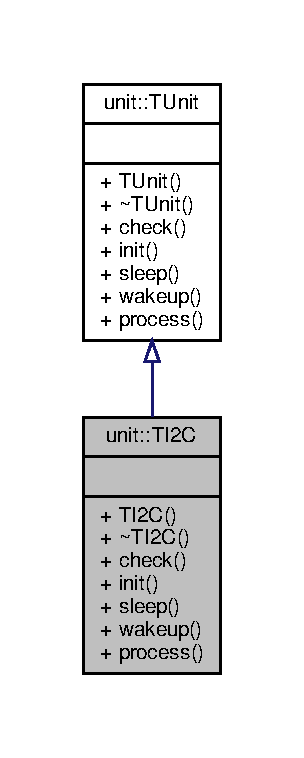
\includegraphics[width=146pt]{classunit_1_1_t_i2_c__inherit__graph}
\end{center}
\end{figure}


Граф связей класса unit\+:\+:T\+I2C\+:\nopagebreak
\begin{figure}[H]
\begin{center}
\leavevmode
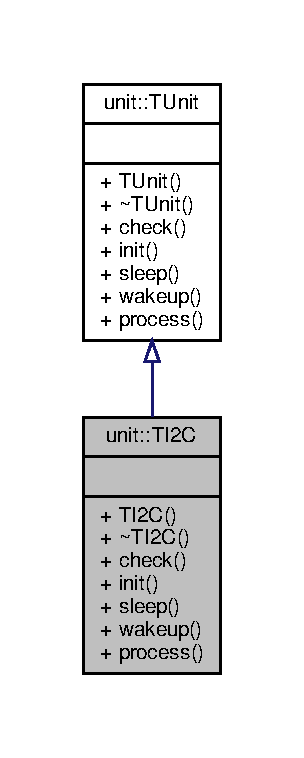
\includegraphics[width=146pt]{classunit_1_1_t_i2_c__coll__graph}
\end{center}
\end{figure}
\subsection*{Открытые члены}
\begin{DoxyCompactItemize}
\item 
bool \hyperlink{classunit_1_1_t_i2_c_a9c392b005548ff42ea8bb0b2255f3779}{check} ()
\begin{DoxyCompactList}\small\item\em Проверка шины i2c. \end{DoxyCompactList}\item 
\mbox{\Hypertarget{classunit_1_1_t_i2_c_a46f9d970fea74ff43f651c92d51cbd7b}\label{classunit_1_1_t_i2_c_a46f9d970fea74ff43f651c92d51cbd7b}} 
void \hyperlink{classunit_1_1_t_i2_c_a46f9d970fea74ff43f651c92d51cbd7b}{init} ()
\begin{DoxyCompactList}\small\item\em Инициализация устройства \end{DoxyCompactList}\item 
\mbox{\Hypertarget{classunit_1_1_t_i2_c_a41cbc4e99cb054156f912d69f84c33e6}\label{classunit_1_1_t_i2_c_a41cbc4e99cb054156f912d69f84c33e6}} 
void \hyperlink{classunit_1_1_t_i2_c_a41cbc4e99cb054156f912d69f84c33e6}{sleep} ()
\begin{DoxyCompactList}\small\item\em Перевод в режим энергосбережения \end{DoxyCompactList}\item 
\mbox{\Hypertarget{classunit_1_1_t_i2_c_a976bf21ac417f9c8301ca5501c3b1c34}\label{classunit_1_1_t_i2_c_a976bf21ac417f9c8301ca5501c3b1c34}} 
void \hyperlink{classunit_1_1_t_i2_c_a976bf21ac417f9c8301ca5501c3b1c34}{wakeup} ()
\begin{DoxyCompactList}\small\item\em Выход из режима энергосбережения \end{DoxyCompactList}\item 
\mbox{\Hypertarget{classunit_1_1_t_i2_c_a246ec834efdab90310976fb19f8047cb}\label{classunit_1_1_t_i2_c_a246ec834efdab90310976fb19f8047cb}} 
bool \hyperlink{classunit_1_1_t_i2_c_a246ec834efdab90310976fb19f8047cb}{process} ()
\begin{DoxyCompactList}\small\item\em Получение данных \end{DoxyCompactList}\end{DoxyCompactItemize}


\subsection{Подробное описание}
Класс для проверки работы шины i2c. И на хрена я это сделел??? \+:( 

\subsection{Методы}
\mbox{\Hypertarget{classunit_1_1_t_i2_c_a9c392b005548ff42ea8bb0b2255f3779}\label{classunit_1_1_t_i2_c_a9c392b005548ff42ea8bb0b2255f3779}} 
\index{unit\+::\+T\+I2C@{unit\+::\+T\+I2C}!check@{check}}
\index{check@{check}!unit\+::\+T\+I2C@{unit\+::\+T\+I2C}}
\subsubsection{\texorpdfstring{check()}{check()}}
{\footnotesize\ttfamily bool unit\+::\+T\+I2\+C\+::check (\begin{DoxyParamCaption}{ }\end{DoxyParamCaption})\hspace{0.3cm}{\ttfamily [virtual]}}



Проверка шины i2c. 

\begin{DoxyReturn}{Возвращает}
При успешной проверке возвращает true ; 
\end{DoxyReturn}


Замещает \hyperlink{classunit_1_1_t_unit_abdcc6daabc86cea10abc96593d9d2c2a}{unit\+::\+T\+Unit}.



Объявления и описания членов классов находятся в файлах\+:\begin{DoxyCompactItemize}
\item 
Core/cpp/T\+I2\+C.\+hpp\item 
Core/cpp/T\+I2\+C.\+cpp\end{DoxyCompactItemize}

\hypertarget{classapp_1_1_t_log}{}\section{Класс app\+:\+:T\+Log}
\label{classapp_1_1_t_log}\index{app\+::\+T\+Log@{app\+::\+T\+Log}}


Класс ведения лога работы  




{\ttfamily \#include $<$T\+Log.\+hpp$>$}



Граф связей класса app\+:\+:T\+Log\+:\nopagebreak
\begin{figure}[H]
\begin{center}
\leavevmode
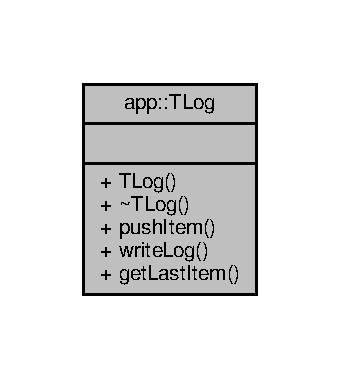
\includegraphics[width=152pt]{classapp_1_1_t_log__coll__graph}
\end{center}
\end{figure}
\subsection*{Открытые члены}
\begin{DoxyCompactItemize}
\item 
\hyperlink{classapp_1_1_t_log_a9f8a10a82504933ab909b90ea9413b65}{T\+Log} ()
\item 
void \hyperlink{classapp_1_1_t_log_a9632f9ff3d14bd24d6587f3509fbe9de}{push\+Item} (const \hyperlink{namespaceapp_a290e8080c661e52c2f685fd4af148acf}{app\+::app\+State} \&)
\begin{DoxyCompactList}\small\item\em Запись в лог изменения состояния \end{DoxyCompactList}\item 
\mbox{\Hypertarget{classapp_1_1_t_log_aa28e5b94b906fcb2f8fed5f08b92e077}\label{classapp_1_1_t_log_aa28e5b94b906fcb2f8fed5f08b92e077}} 
bool \hyperlink{classapp_1_1_t_log_aa28e5b94b906fcb2f8fed5f08b92e077}{write\+Log} ()
\begin{DoxyCompactList}\small\item\em Сохранение лога на флешку и если нужно на S\+D\+IO. Всегда записывается последний банк встроенной флешки \end{DoxyCompactList}\end{DoxyCompactItemize}


\subsection{Подробное описание}
Класс ведения лога работы 

Все события пишутся в контейнер std\+::deque, т.\+к. std\+::queue кривой и записываются в последний банк флешки при переходе в состояние Stand\+By. При начале активности последнее событие пишется в контейнер и если первое и последнее событие == app\+State\+::app\+Hw\+Err, то запись на флешку не производится. Т.\+о. мы убираем поток ошибок при падении по памяти Что бы не взрывать себе мозги, указатель на пустое место для записи хранится в регистре R\+T\+C\+\_\+\+B\+K\+P\+\_\+\+D\+R1 \begin{DoxyRefDesc}{Необходимо сделать}
\item[\hyperlink{todo__todo000009}{Необходимо сделать}]Переделать на запись на SD карточку. 

Написать класс для работы с встроенной флешкой \end{DoxyRefDesc}


\subsection{Конструктор(ы)}
\mbox{\Hypertarget{classapp_1_1_t_log_a9f8a10a82504933ab909b90ea9413b65}\label{classapp_1_1_t_log_a9f8a10a82504933ab909b90ea9413b65}} 
\index{app\+::\+T\+Log@{app\+::\+T\+Log}!T\+Log@{T\+Log}}
\index{T\+Log@{T\+Log}!app\+::\+T\+Log@{app\+::\+T\+Log}}
\subsubsection{\texorpdfstring{T\+Log()}{TLog()}}
{\footnotesize\ttfamily app\+::\+T\+Log\+::\+T\+Log (\begin{DoxyParamCaption}{ }\end{DoxyParamCaption})}



 

\subsection{Методы}
\mbox{\Hypertarget{classapp_1_1_t_log_a9632f9ff3d14bd24d6587f3509fbe9de}\label{classapp_1_1_t_log_a9632f9ff3d14bd24d6587f3509fbe9de}} 
\index{app\+::\+T\+Log@{app\+::\+T\+Log}!push\+Item@{push\+Item}}
\index{push\+Item@{push\+Item}!app\+::\+T\+Log@{app\+::\+T\+Log}}
\subsubsection{\texorpdfstring{push\+Item()}{pushItem()}}
{\footnotesize\ttfamily void app\+::\+T\+Log\+::push\+Item (\begin{DoxyParamCaption}\item[{const \hyperlink{namespaceapp_a290e8080c661e52c2f685fd4af148acf}{app\+::app\+State} \&}]{in\+State }\end{DoxyParamCaption})}



Запись в лог изменения состояния 

Формирование очереди сообщений которые нужно записывать в лог. Новые сообщения пишутся в конец (push\+\_\+back) По хорошему, можно использовать std\+::vector и писать флешку всё сразу массивом ...data, но хрен его знает, что будет при динамическом выделении памяти. \+:( 
\begin{DoxyParams}{Аргументы}
{\em in\+State} & записываемое состояние \\
\hline
\end{DoxyParams}


Объявления и описания членов классов находятся в файлах\+:\begin{DoxyCompactItemize}
\item 
Core/cpp/T\+Log.\+hpp\item 
Core/cpp/T\+Log.\+cpp\end{DoxyCompactItemize}

\hypertarget{classunit_1_1_t_photo}{}\section{Класс unit\+:\+:T\+Photo}
\label{classunit_1_1_t_photo}\index{unit\+::\+T\+Photo@{unit\+::\+T\+Photo}}


{\ttfamily \#include $<$T\+Photo.\+hpp$>$}



Граф наследования\+:unit\+:\+:T\+Photo\+:\nopagebreak
\begin{figure}[H]
\begin{center}
\leavevmode
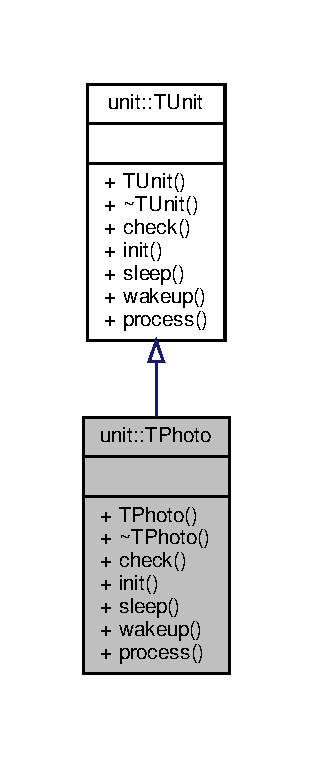
\includegraphics[width=150pt]{classunit_1_1_t_photo__inherit__graph}
\end{center}
\end{figure}


Граф связей класса unit\+:\+:T\+Photo\+:\nopagebreak
\begin{figure}[H]
\begin{center}
\leavevmode
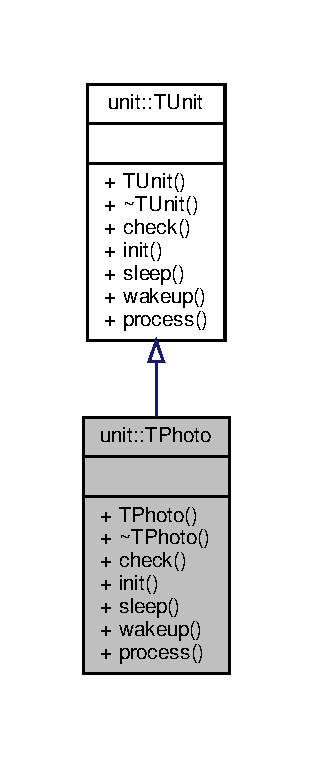
\includegraphics[width=150pt]{classunit_1_1_t_photo__coll__graph}
\end{center}
\end{figure}
\subsection*{Открытые члены}
\begin{DoxyCompactItemize}
\item 
\hyperlink{classunit_1_1_t_photo_ac4d5d37e712767fa9b899648949b2ef3}{T\+Photo} ()
\item 
virtual \hyperlink{classunit_1_1_t_photo_a1c9c83e03a16b4e66a0fc48f734a5b93}{$\sim$\+T\+Photo} ()
\item 
bool \hyperlink{classunit_1_1_t_photo_a292ed1d6e9fb0b8335234891716eec8d}{check} ()
\begin{DoxyCompactList}\small\item\em Проверка оборудования \end{DoxyCompactList}\item 
void \hyperlink{classunit_1_1_t_photo_adfad75bd5d77ef72f526cc43474c3d87}{init} ()
\begin{DoxyCompactList}\small\item\em Инициализация устройства \end{DoxyCompactList}\item 
void \hyperlink{classunit_1_1_t_photo_acfdae485260a64864e779cacd15644f7}{sleep} ()
\begin{DoxyCompactList}\small\item\em Перевод в режим энергосбережения \end{DoxyCompactList}\item 
void \hyperlink{classunit_1_1_t_photo_a2d8ecace1e51abed1a68731b486680f6}{wakeup} ()
\begin{DoxyCompactList}\small\item\em Выход из режима энергосбережения \end{DoxyCompactList}\item 
bool \hyperlink{classunit_1_1_t_photo_a8323fa27bff29d883e9903b74c341605}{process} ()
\begin{DoxyCompactList}\small\item\em Получение изображения с камеры и запись его в файл \end{DoxyCompactList}\end{DoxyCompactItemize}


\subsection{Подробное описание}
Класс работы с камерой O\+V2640 \begin{DoxyRefDesc}{Необходимо сделать}
\item[\hyperlink{todo__todo000012}{Необходимо сделать}]Убрать ov2640.\+c и передалать на плюсы (Хотя не очень понятно зачем???) 

Убрать все Warning в ov2640.\+c \end{DoxyRefDesc}


\subsection{Конструктор(ы)}
\mbox{\Hypertarget{classunit_1_1_t_photo_ac4d5d37e712767fa9b899648949b2ef3}\label{classunit_1_1_t_photo_ac4d5d37e712767fa9b899648949b2ef3}} 
\index{unit\+::\+T\+Photo@{unit\+::\+T\+Photo}!T\+Photo@{T\+Photo}}
\index{T\+Photo@{T\+Photo}!unit\+::\+T\+Photo@{unit\+::\+T\+Photo}}
\subsubsection{\texorpdfstring{T\+Photo()}{TPhoto()}}
{\footnotesize\ttfamily unit\+::\+T\+Photo\+::\+T\+Photo (\begin{DoxyParamCaption}{ }\end{DoxyParamCaption})}



 Конструктор инициализирующий камеру Граф вызовов\+:\nopagebreak
\begin{figure}[H]
\begin{center}
\leavevmode
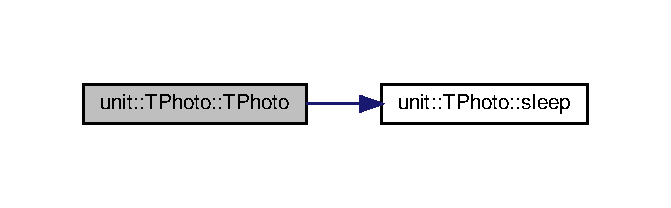
\includegraphics[width=312pt]{classunit_1_1_t_photo_ac4d5d37e712767fa9b899648949b2ef3_cgraph}
\end{center}
\end{figure}
\mbox{\Hypertarget{classunit_1_1_t_photo_a1c9c83e03a16b4e66a0fc48f734a5b93}\label{classunit_1_1_t_photo_a1c9c83e03a16b4e66a0fc48f734a5b93}} 
\index{unit\+::\+T\+Photo@{unit\+::\+T\+Photo}!````~T\+Photo@{$\sim$\+T\+Photo}}
\index{````~T\+Photo@{$\sim$\+T\+Photo}!unit\+::\+T\+Photo@{unit\+::\+T\+Photo}}
\subsubsection{\texorpdfstring{$\sim$\+T\+Photo()}{~TPhoto()}}
{\footnotesize\ttfamily unit\+::\+T\+Photo\+::$\sim$\+T\+Photo (\begin{DoxyParamCaption}{ }\end{DoxyParamCaption})\hspace{0.3cm}{\ttfamily [virtual]}}



 Граф вызовов\+:\nopagebreak
\begin{figure}[H]
\begin{center}
\leavevmode
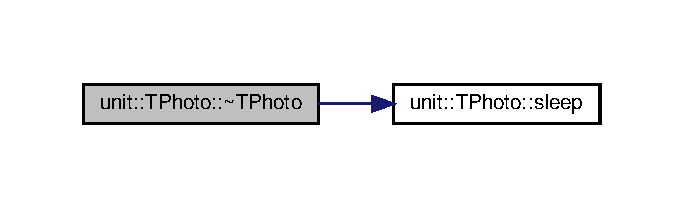
\includegraphics[width=328pt]{classunit_1_1_t_photo_a1c9c83e03a16b4e66a0fc48f734a5b93_cgraph}
\end{center}
\end{figure}


\subsection{Методы}
\mbox{\Hypertarget{classunit_1_1_t_photo_a292ed1d6e9fb0b8335234891716eec8d}\label{classunit_1_1_t_photo_a292ed1d6e9fb0b8335234891716eec8d}} 
\index{unit\+::\+T\+Photo@{unit\+::\+T\+Photo}!check@{check}}
\index{check@{check}!unit\+::\+T\+Photo@{unit\+::\+T\+Photo}}
\subsubsection{\texorpdfstring{check()}{check()}}
{\footnotesize\ttfamily bool unit\+::\+T\+Photo\+::check (\begin{DoxyParamCaption}{ }\end{DoxyParamCaption})\hspace{0.3cm}{\ttfamily [virtual]}}



Проверка оборудования 





\begin{DoxyReturn}{Возвращает}
При успешной проверке возвращается true 
\end{DoxyReturn}


Замещает \hyperlink{classunit_1_1_t_unit_abdcc6daabc86cea10abc96593d9d2c2a}{unit\+::\+T\+Unit}.

\mbox{\Hypertarget{classunit_1_1_t_photo_adfad75bd5d77ef72f526cc43474c3d87}\label{classunit_1_1_t_photo_adfad75bd5d77ef72f526cc43474c3d87}} 
\index{unit\+::\+T\+Photo@{unit\+::\+T\+Photo}!init@{init}}
\index{init@{init}!unit\+::\+T\+Photo@{unit\+::\+T\+Photo}}
\subsubsection{\texorpdfstring{init()}{init()}}
{\footnotesize\ttfamily void unit\+::\+T\+Photo\+::init (\begin{DoxyParamCaption}{ }\end{DoxyParamCaption})\hspace{0.3cm}{\ttfamily [virtual]}}



Инициализация устройства 



 Задаются все конфигурацилнные настройки 

Замещает \hyperlink{classunit_1_1_t_unit_afc001dd57ba88e571e6b650a416b76a5}{unit\+::\+T\+Unit}.

\mbox{\Hypertarget{classunit_1_1_t_photo_a8323fa27bff29d883e9903b74c341605}\label{classunit_1_1_t_photo_a8323fa27bff29d883e9903b74c341605}} 
\index{unit\+::\+T\+Photo@{unit\+::\+T\+Photo}!process@{process}}
\index{process@{process}!unit\+::\+T\+Photo@{unit\+::\+T\+Photo}}
\subsubsection{\texorpdfstring{process()}{process()}}
{\footnotesize\ttfamily bool unit\+::\+T\+Photo\+::process (\begin{DoxyParamCaption}{ }\end{DoxyParamCaption})\hspace{0.3cm}{\ttfamily [virtual]}}



Получение изображения с камеры и запись его в файл 



 \begin{DoxyAttention}{Внимание}
Я ни коим образом не проверяю корректность инициализации и возвращаемые ошибки!!! 
\end{DoxyAttention}
\begin{DoxyRefDesc}{Необходимо сделать}
\item[\hyperlink{todo__todo000011}{Необходимо сделать}]Переделать ожидание получения изображения \end{DoxyRefDesc}


Замещает \hyperlink{classunit_1_1_t_unit_a108691c8b988d97c65237c83a31db706}{unit\+::\+T\+Unit}.

Граф вызовов\+:\nopagebreak
\begin{figure}[H]
\begin{center}
\leavevmode
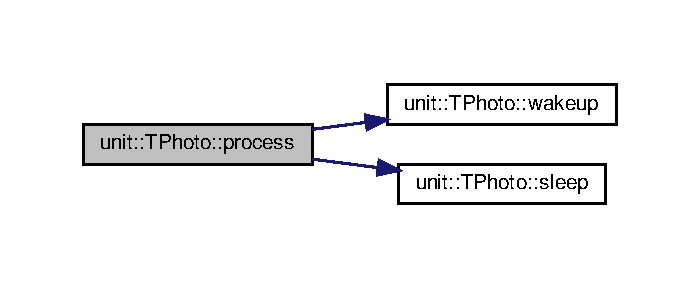
\includegraphics[width=336pt]{classunit_1_1_t_photo_a8323fa27bff29d883e9903b74c341605_cgraph}
\end{center}
\end{figure}
\mbox{\Hypertarget{classunit_1_1_t_photo_acfdae485260a64864e779cacd15644f7}\label{classunit_1_1_t_photo_acfdae485260a64864e779cacd15644f7}} 
\index{unit\+::\+T\+Photo@{unit\+::\+T\+Photo}!sleep@{sleep}}
\index{sleep@{sleep}!unit\+::\+T\+Photo@{unit\+::\+T\+Photo}}
\subsubsection{\texorpdfstring{sleep()}{sleep()}}
{\footnotesize\ttfamily void unit\+::\+T\+Photo\+::sleep (\begin{DoxyParamCaption}{ }\end{DoxyParamCaption})\hspace{0.3cm}{\ttfamily [virtual]}}



Перевод в режим энергосбережения 



 

Замещает \hyperlink{classunit_1_1_t_unit_afa851323a357e4287ca230d2bce8977b}{unit\+::\+T\+Unit}.

\mbox{\Hypertarget{classunit_1_1_t_photo_a2d8ecace1e51abed1a68731b486680f6}\label{classunit_1_1_t_photo_a2d8ecace1e51abed1a68731b486680f6}} 
\index{unit\+::\+T\+Photo@{unit\+::\+T\+Photo}!wakeup@{wakeup}}
\index{wakeup@{wakeup}!unit\+::\+T\+Photo@{unit\+::\+T\+Photo}}
\subsubsection{\texorpdfstring{wakeup()}{wakeup()}}
{\footnotesize\ttfamily void unit\+::\+T\+Photo\+::wakeup (\begin{DoxyParamCaption}{ }\end{DoxyParamCaption})\hspace{0.3cm}{\ttfamily [virtual]}}



Выход из режима энергосбережения 



 

Замещает \hyperlink{classunit_1_1_t_unit_a11fd67d0186e8e60ef517d6a44db225f}{unit\+::\+T\+Unit}.



Объявления и описания членов классов находятся в файлах\+:\begin{DoxyCompactItemize}
\item 
Core/cpp/T\+Photo.\+hpp\item 
Core/cpp/T\+Photo.\+cpp\end{DoxyCompactItemize}

\hypertarget{classunit_1_1_t_sdio}{}\section{Класс unit\+:\+:T\+Sdio}
\label{classunit_1_1_t_sdio}\index{unit\+::\+T\+Sdio@{unit\+::\+T\+Sdio}}


Граф наследования\+:unit\+:\+:T\+Sdio\+:\nopagebreak
\begin{figure}[H]
\begin{center}
\leavevmode
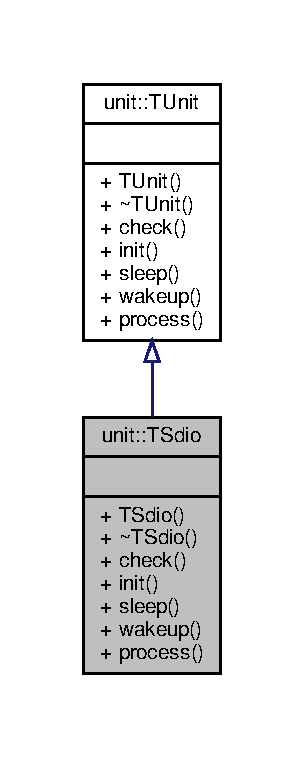
\includegraphics[width=146pt]{classunit_1_1_t_sdio__inherit__graph}
\end{center}
\end{figure}


Граф связей класса unit\+:\+:T\+Sdio\+:\nopagebreak
\begin{figure}[H]
\begin{center}
\leavevmode
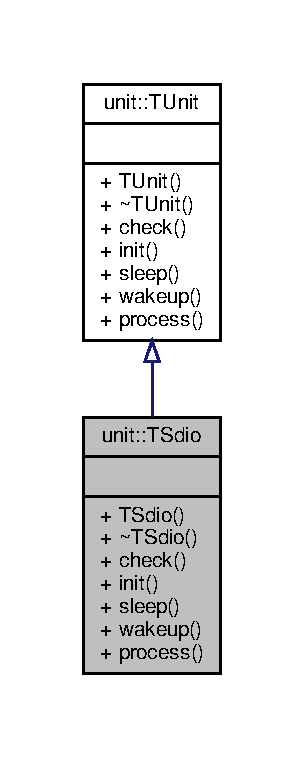
\includegraphics[width=146pt]{classunit_1_1_t_sdio__coll__graph}
\end{center}
\end{figure}
\subsection*{Открытые члены}
\begin{DoxyCompactItemize}
\item 
\hyperlink{classunit_1_1_t_sdio_ab772a88df605f6d22e9352d281bc7e08}{T\+Sdio} ()
\item 
bool \hyperlink{classunit_1_1_t_sdio_a01d0b69d4bf6735a74efc1a4661289e7}{check} ()
\begin{DoxyCompactList}\small\item\em Проверка работоспособности S\+D\+IO. \end{DoxyCompactList}\item 
\mbox{\Hypertarget{classunit_1_1_t_sdio_a003c079fd0ca2cf186b17e51fd2c8c56}\label{classunit_1_1_t_sdio_a003c079fd0ca2cf186b17e51fd2c8c56}} 
void \hyperlink{classunit_1_1_t_sdio_a003c079fd0ca2cf186b17e51fd2c8c56}{init} ()
\begin{DoxyCompactList}\small\item\em Инициализация устройства \end{DoxyCompactList}\item 
\mbox{\Hypertarget{classunit_1_1_t_sdio_ac903a19ed873242ad2da15224b3925fa}\label{classunit_1_1_t_sdio_ac903a19ed873242ad2da15224b3925fa}} 
void \hyperlink{classunit_1_1_t_sdio_ac903a19ed873242ad2da15224b3925fa}{sleep} ()
\begin{DoxyCompactList}\small\item\em Перевод в режим энергосбережения \end{DoxyCompactList}\item 
\mbox{\Hypertarget{classunit_1_1_t_sdio_ae2af97f7a50c9bcc53132ab379fd5c25}\label{classunit_1_1_t_sdio_ae2af97f7a50c9bcc53132ab379fd5c25}} 
void \hyperlink{classunit_1_1_t_sdio_ae2af97f7a50c9bcc53132ab379fd5c25}{wakeup} ()
\begin{DoxyCompactList}\small\item\em Выход из режима энергосбережения \end{DoxyCompactList}\item 
\mbox{\Hypertarget{classunit_1_1_t_sdio_a0ae751c5761bfbafdfa977617a43283b}\label{classunit_1_1_t_sdio_a0ae751c5761bfbafdfa977617a43283b}} 
bool \hyperlink{classunit_1_1_t_sdio_a0ae751c5761bfbafdfa977617a43283b}{process} ()
\begin{DoxyCompactList}\small\item\em Получение данных \end{DoxyCompactList}\end{DoxyCompactItemize}


\subsection{Конструктор(ы)}
\mbox{\Hypertarget{classunit_1_1_t_sdio_ab772a88df605f6d22e9352d281bc7e08}\label{classunit_1_1_t_sdio_ab772a88df605f6d22e9352d281bc7e08}} 
\index{unit\+::\+T\+Sdio@{unit\+::\+T\+Sdio}!T\+Sdio@{T\+Sdio}}
\index{T\+Sdio@{T\+Sdio}!unit\+::\+T\+Sdio@{unit\+::\+T\+Sdio}}
\subsubsection{\texorpdfstring{T\+Sdio()}{TSdio()}}
{\footnotesize\ttfamily unit\+::\+T\+Sdio\+::\+T\+Sdio (\begin{DoxyParamCaption}{ }\end{DoxyParamCaption})}

\begin{DoxyAttention}{Внимание}
Нет проверки инициализирована SD карточка или нет!!! 
\end{DoxyAttention}


\subsection{Методы}
\mbox{\Hypertarget{classunit_1_1_t_sdio_a01d0b69d4bf6735a74efc1a4661289e7}\label{classunit_1_1_t_sdio_a01d0b69d4bf6735a74efc1a4661289e7}} 
\index{unit\+::\+T\+Sdio@{unit\+::\+T\+Sdio}!check@{check}}
\index{check@{check}!unit\+::\+T\+Sdio@{unit\+::\+T\+Sdio}}
\subsubsection{\texorpdfstring{check()}{check()}}
{\footnotesize\ttfamily bool unit\+::\+T\+Sdio\+::check (\begin{DoxyParamCaption}{ }\end{DoxyParamCaption})\hspace{0.3cm}{\ttfamily [virtual]}}



Проверка работоспособности S\+D\+IO. 

\begin{DoxyReturn}{Возвращает}
Если все Ok, то возвращается true 
\end{DoxyReturn}


Замещает \hyperlink{classunit_1_1_t_unit_abdcc6daabc86cea10abc96593d9d2c2a}{unit\+::\+T\+Unit}.



Объявления и описания членов классов находятся в файлах\+:\begin{DoxyCompactItemize}
\item 
Core/cpp/T\+Sdio.\+hpp\item 
Core/cpp/T\+Sdio.\+cpp\end{DoxyCompactItemize}

\hypertarget{classunit_1_1_t_tag}{}\section{Класс unit\+:\+:T\+Tag}
\label{classunit_1_1_t_tag}\index{unit\+::\+T\+Tag@{unit\+::\+T\+Tag}}


{\ttfamily \#include $<$T\+Tag.\+hpp$>$}



Граф наследования\+:unit\+:\+:T\+Tag\+:\nopagebreak
\begin{figure}[H]
\begin{center}
\leavevmode
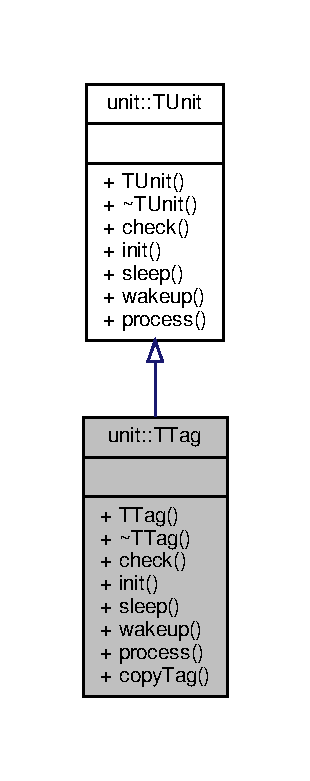
\includegraphics[width=149pt]{classunit_1_1_t_tag__inherit__graph}
\end{center}
\end{figure}


Граф связей класса unit\+:\+:T\+Tag\+:\nopagebreak
\begin{figure}[H]
\begin{center}
\leavevmode
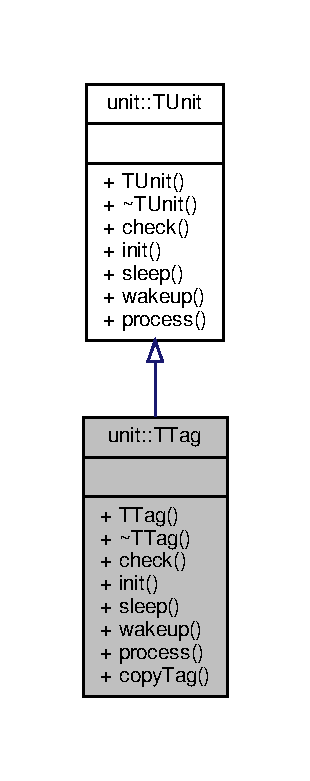
\includegraphics[width=149pt]{classunit_1_1_t_tag__coll__graph}
\end{center}
\end{figure}
\subsection*{Открытые члены}
\begin{DoxyCompactItemize}
\item 
\mbox{\Hypertarget{classunit_1_1_t_tag_adc2c2801738b094045529f1373f28203}\label{classunit_1_1_t_tag_adc2c2801738b094045529f1373f28203}} 
bool \hyperlink{classunit_1_1_t_tag_adc2c2801738b094045529f1373f28203}{check} ()
\begin{DoxyCompactList}\small\item\em Проверка оборудования \end{DoxyCompactList}\item 
\mbox{\Hypertarget{classunit_1_1_t_tag_ae3158aefc30472351d25cfba3c3f0b9f}\label{classunit_1_1_t_tag_ae3158aefc30472351d25cfba3c3f0b9f}} 
void \hyperlink{classunit_1_1_t_tag_ae3158aefc30472351d25cfba3c3f0b9f}{init} ()
\begin{DoxyCompactList}\small\item\em Инициализация устройства \end{DoxyCompactList}\item 
\mbox{\Hypertarget{classunit_1_1_t_tag_acd600380312d44954f0b46ec5f704691}\label{classunit_1_1_t_tag_acd600380312d44954f0b46ec5f704691}} 
void \hyperlink{classunit_1_1_t_tag_acd600380312d44954f0b46ec5f704691}{sleep} ()
\begin{DoxyCompactList}\small\item\em Перевод в режим энергосбережения \end{DoxyCompactList}\item 
\mbox{\Hypertarget{classunit_1_1_t_tag_afc0b9080d0c67ed9fbdaa4ae3bfdfc7c}\label{classunit_1_1_t_tag_afc0b9080d0c67ed9fbdaa4ae3bfdfc7c}} 
void \hyperlink{classunit_1_1_t_tag_afc0b9080d0c67ed9fbdaa4ae3bfdfc7c}{wakeup} ()
\begin{DoxyCompactList}\small\item\em Выход из режима энергосбережения \end{DoxyCompactList}\item 
bool \hyperlink{classunit_1_1_t_tag_a1dfd588909730d0b48edbeda273526fe}{process} ()
\begin{DoxyCompactList}\small\item\em Чтения метки \end{DoxyCompactList}\item 
void \hyperlink{classunit_1_1_t_tag_a90fba846800afa1b828d81f079ba735e}{copy\+Tag} (uint8\+\_\+t $\ast$)
\begin{DoxyCompactList}\small\item\em Копирование текущей метки из регистра R\+T\+C\+\_\+\+B\+K\+P\+\_\+\+D\+R0 в uint8\+\_\+t буфер \end{DoxyCompactList}\end{DoxyCompactItemize}


\subsection{Подробное описание}
Класс управления чипом P\+N532 Считанная метка записывается в backup регистр R\+T\+C\+\_\+\+B\+K\+P\+\_\+\+D\+R0 и доступна всегда. 

\subsection{Методы}
\mbox{\Hypertarget{classunit_1_1_t_tag_a90fba846800afa1b828d81f079ba735e}\label{classunit_1_1_t_tag_a90fba846800afa1b828d81f079ba735e}} 
\index{unit\+::\+T\+Tag@{unit\+::\+T\+Tag}!copy\+Tag@{copy\+Tag}}
\index{copy\+Tag@{copy\+Tag}!unit\+::\+T\+Tag@{unit\+::\+T\+Tag}}
\subsubsection{\texorpdfstring{copy\+Tag()}{copyTag()}}
{\footnotesize\ttfamily void unit\+::\+T\+Tag\+::copy\+Tag (\begin{DoxyParamCaption}\item[{uint8\+\_\+t $\ast$}]{in\+Ptr }\end{DoxyParamCaption})}



Копирование текущей метки из регистра R\+T\+C\+\_\+\+B\+K\+P\+\_\+\+D\+R0 в uint8\+\_\+t буфер 



 
\begin{DoxyParams}{Аргументы}
{\em in\+Ptr} & Указатель куда копируем метку \\
\hline
\end{DoxyParams}
\mbox{\Hypertarget{classunit_1_1_t_tag_a1dfd588909730d0b48edbeda273526fe}\label{classunit_1_1_t_tag_a1dfd588909730d0b48edbeda273526fe}} 
\index{unit\+::\+T\+Tag@{unit\+::\+T\+Tag}!process@{process}}
\index{process@{process}!unit\+::\+T\+Tag@{unit\+::\+T\+Tag}}
\subsubsection{\texorpdfstring{process()}{process()}}
{\footnotesize\ttfamily bool unit\+::\+T\+Tag\+::process (\begin{DoxyParamCaption}{ }\end{DoxyParamCaption})\hspace{0.3cm}{\ttfamily [virtual]}}



Чтения метки 

Метод сканирует метку и записывает ее в регистр \begin{DoxyReturn}{Возвращает}
При успешном сканировании возвращает true 
\end{DoxyReturn}


Замещает \hyperlink{classunit_1_1_t_unit_a108691c8b988d97c65237c83a31db706}{unit\+::\+T\+Unit}.

Граф вызовов\+:\nopagebreak
\begin{figure}[H]
\begin{center}
\leavevmode
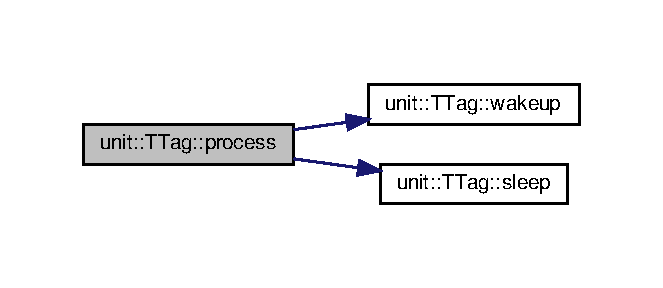
\includegraphics[width=318pt]{classunit_1_1_t_tag_a1dfd588909730d0b48edbeda273526fe_cgraph}
\end{center}
\end{figure}


Объявления и описания членов классов находятся в файлах\+:\begin{DoxyCompactItemize}
\item 
Core/cpp/T\+Tag.\+hpp\item 
Core/cpp/T\+Tag.\+cpp\end{DoxyCompactItemize}

\hypertarget{classunit_1_1_t_unit}{}\section{Класс unit\+:\+:T\+Unit}
\label{classunit_1_1_t_unit}\index{unit\+::\+T\+Unit@{unit\+::\+T\+Unit}}


{\ttfamily \#include $<$T\+Unit.\+hpp$>$}



Граф наследования\+:unit\+:\+:T\+Unit\+:\nopagebreak
\begin{figure}[H]
\begin{center}
\leavevmode
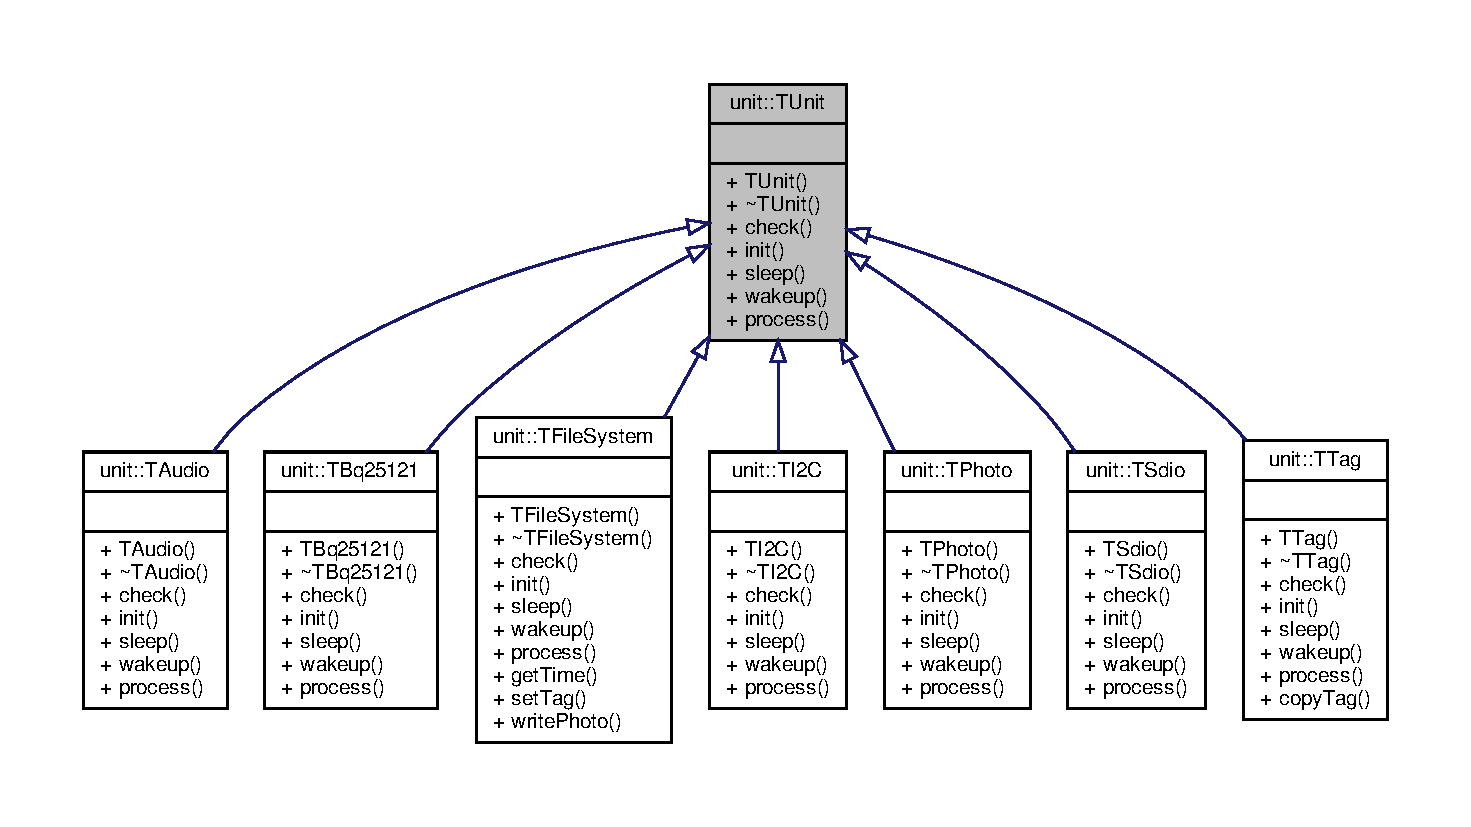
\includegraphics[width=350pt]{classunit_1_1_t_unit__inherit__graph}
\end{center}
\end{figure}


Граф связей класса unit\+:\+:T\+Unit\+:\nopagebreak
\begin{figure}[H]
\begin{center}
\leavevmode
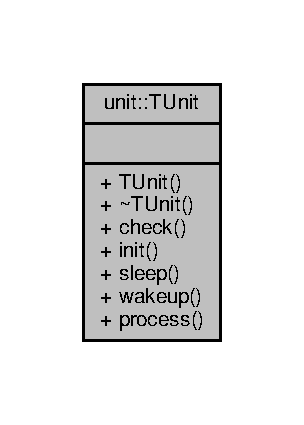
\includegraphics[width=146pt]{classunit_1_1_t_unit__coll__graph}
\end{center}
\end{figure}
\subsection*{Открытые члены}
\begin{DoxyCompactItemize}
\item 
\mbox{\Hypertarget{classunit_1_1_t_unit_abdcc6daabc86cea10abc96593d9d2c2a}\label{classunit_1_1_t_unit_abdcc6daabc86cea10abc96593d9d2c2a}} 
virtual bool \hyperlink{classunit_1_1_t_unit_abdcc6daabc86cea10abc96593d9d2c2a}{check} ()=0
\begin{DoxyCompactList}\small\item\em Проверка оборудования устройства \end{DoxyCompactList}\item 
\mbox{\Hypertarget{classunit_1_1_t_unit_afc001dd57ba88e571e6b650a416b76a5}\label{classunit_1_1_t_unit_afc001dd57ba88e571e6b650a416b76a5}} 
virtual void \hyperlink{classunit_1_1_t_unit_afc001dd57ba88e571e6b650a416b76a5}{init} ()=0
\begin{DoxyCompactList}\small\item\em Инициализация устройства \end{DoxyCompactList}\item 
\mbox{\Hypertarget{classunit_1_1_t_unit_afa851323a357e4287ca230d2bce8977b}\label{classunit_1_1_t_unit_afa851323a357e4287ca230d2bce8977b}} 
virtual void \hyperlink{classunit_1_1_t_unit_afa851323a357e4287ca230d2bce8977b}{sleep} ()=0
\begin{DoxyCompactList}\small\item\em Перевод в режим энергосбережения \end{DoxyCompactList}\item 
\mbox{\Hypertarget{classunit_1_1_t_unit_a11fd67d0186e8e60ef517d6a44db225f}\label{classunit_1_1_t_unit_a11fd67d0186e8e60ef517d6a44db225f}} 
virtual void \hyperlink{classunit_1_1_t_unit_a11fd67d0186e8e60ef517d6a44db225f}{wakeup} ()=0
\begin{DoxyCompactList}\small\item\em Выход из режима энергосбережения \end{DoxyCompactList}\item 
\mbox{\Hypertarget{classunit_1_1_t_unit_a108691c8b988d97c65237c83a31db706}\label{classunit_1_1_t_unit_a108691c8b988d97c65237c83a31db706}} 
virtual bool \hyperlink{classunit_1_1_t_unit_a108691c8b988d97c65237c83a31db706}{process} ()=0
\begin{DoxyCompactList}\small\item\em Получение данных \end{DoxyCompactList}\end{DoxyCompactItemize}


\subsection{Подробное описание}
Базовый класс для работы с периферийным оборудованием 

Объявления и описания членов класса находятся в файле\+:\begin{DoxyCompactItemize}
\item 
Core/cpp/T\+Unit.\+hpp\end{DoxyCompactItemize}

\hypertarget{struct_w_a_v_e___format_type_def}{}\section{Структура W\+A\+V\+E\+\_\+\+Format\+Type\+Def}
\label{struct_w_a_v_e___format_type_def}\index{W\+A\+V\+E\+\_\+\+Format\+Type\+Def@{W\+A\+V\+E\+\_\+\+Format\+Type\+Def}}


Граф связей класса W\+A\+V\+E\+\_\+\+Format\+Type\+Def\+:\nopagebreak
\begin{figure}[H]
\begin{center}
\leavevmode
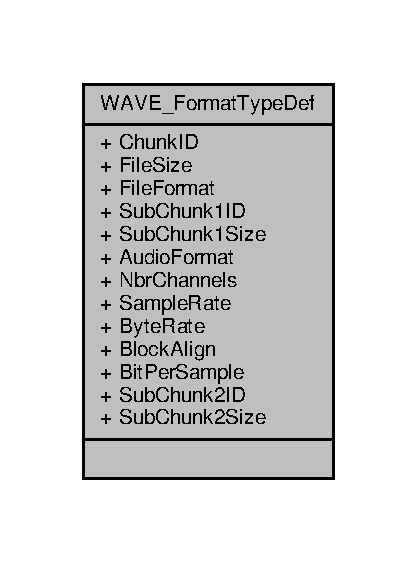
\includegraphics[width=200pt]{struct_w_a_v_e___format_type_def__coll__graph}
\end{center}
\end{figure}
\subsection*{Открытые атрибуты}
\begin{DoxyCompactItemize}
\item 
\mbox{\Hypertarget{struct_w_a_v_e___format_type_def_a9e56c5528ba5f964ea9a6dbd4d0e1682}\label{struct_w_a_v_e___format_type_def_a9e56c5528ba5f964ea9a6dbd4d0e1682}} 
const uint32\+\_\+t {\bfseries Chunk\+ID} \{ 0x46464952 \}
\item 
\mbox{\Hypertarget{struct_w_a_v_e___format_type_def_ada518c6be3de72904ebafd155ec9630d}\label{struct_w_a_v_e___format_type_def_ada518c6be3de72904ebafd155ec9630d}} 
uint32\+\_\+t {\bfseries File\+Size}
\item 
\mbox{\Hypertarget{struct_w_a_v_e___format_type_def_acad647933f0c40b1d303a397d9f67b4d}\label{struct_w_a_v_e___format_type_def_acad647933f0c40b1d303a397d9f67b4d}} 
const uint32\+\_\+t {\bfseries File\+Format} \{ 0x45564157 \}
\item 
\mbox{\Hypertarget{struct_w_a_v_e___format_type_def_ab5180372ca4a5bcb1775f4c45343eb22}\label{struct_w_a_v_e___format_type_def_ab5180372ca4a5bcb1775f4c45343eb22}} 
const uint32\+\_\+t {\bfseries Sub\+Chunk1\+ID} \{ 0x20746\+D66 \}
\item 
\mbox{\Hypertarget{struct_w_a_v_e___format_type_def_a6a53e86701dc1a4a93630ee3ad53438a}\label{struct_w_a_v_e___format_type_def_a6a53e86701dc1a4a93630ee3ad53438a}} 
const uint32\+\_\+t {\bfseries Sub\+Chunk1\+Size} \{ 0x10 \}
\item 
\mbox{\Hypertarget{struct_w_a_v_e___format_type_def_afa331bc2177f7f7df7d5332b8b9d9d2c}\label{struct_w_a_v_e___format_type_def_afa331bc2177f7f7df7d5332b8b9d9d2c}} 
const uint16\+\_\+t {\bfseries Audio\+Format} \{ 0x1 \}
\item 
\mbox{\Hypertarget{struct_w_a_v_e___format_type_def_acc7e2458d4ca37fbf4acd51475f82b10}\label{struct_w_a_v_e___format_type_def_acc7e2458d4ca37fbf4acd51475f82b10}} 
const uint16\+\_\+t {\bfseries Nbr\+Channels} \{ 0x1 \}
\item 
\mbox{\Hypertarget{struct_w_a_v_e___format_type_def_a672b7e05b22d49864679d9d45367d0ad}\label{struct_w_a_v_e___format_type_def_a672b7e05b22d49864679d9d45367d0ad}} 
const uint32\+\_\+t {\bfseries Sample\+Rate} \{ 0x1\+F40 \}
\item 
\mbox{\Hypertarget{struct_w_a_v_e___format_type_def_a8dc13a7a425fbefd6357b06cc1752234}\label{struct_w_a_v_e___format_type_def_a8dc13a7a425fbefd6357b06cc1752234}} 
const uint32\+\_\+t {\bfseries Byte\+Rate} \{ 0x3\+E80 \}
\item 
\mbox{\Hypertarget{struct_w_a_v_e___format_type_def_a54dbceb93d3c8e6c5fc8abe656814f93}\label{struct_w_a_v_e___format_type_def_a54dbceb93d3c8e6c5fc8abe656814f93}} 
const uint16\+\_\+t {\bfseries Block\+Align} \{ 0x02 \}
\item 
\mbox{\Hypertarget{struct_w_a_v_e___format_type_def_a301883744fb8bcbd48f5330637e56ffc}\label{struct_w_a_v_e___format_type_def_a301883744fb8bcbd48f5330637e56ffc}} 
const uint16\+\_\+t {\bfseries Bit\+Per\+Sample} \{ 0x10 \}
\item 
\mbox{\Hypertarget{struct_w_a_v_e___format_type_def_a775aa21eb108eac6501f57dd8f5f3a3d}\label{struct_w_a_v_e___format_type_def_a775aa21eb108eac6501f57dd8f5f3a3d}} 
const uint32\+\_\+t {\bfseries Sub\+Chunk2\+ID} \{ 0x61746164 \}
\item 
\mbox{\Hypertarget{struct_w_a_v_e___format_type_def_ac5e22f09d20598d46149e2f5d290c0c7}\label{struct_w_a_v_e___format_type_def_ac5e22f09d20598d46149e2f5d290c0c7}} 
uint32\+\_\+t {\bfseries Sub\+Chunk2\+Size}
\end{DoxyCompactItemize}


Объявления и описания членов структуры находятся в файле\+:\begin{DoxyCompactItemize}
\item 
Core/cpp/T\+File\+System.\+hpp\end{DoxyCompactItemize}

%--- End generated contents ---

% Index
\backmatter
\newpage
\phantomsection
\clearemptydoublepage
\addcontentsline{toc}{chapter}{Алфавитный указатель}
\printindex

\end{document}
